\documentclass{FastFyp}
\usepackage{amsmath}
\usepackage{xcolor}
\usepackage{longtable}
\usepackage{array}
\usepackage{needspace}
\usepackage{url}
\usepackage{graphicx}
\usepackage{comment}
\usepackage{float}
\usepackage{placeins}
\usepackage{tabularx}
\usepackage{seqsplit}
\newcommand{\tcbrk}[1]{\seqsplit{#1}}
\begin{document}
\newcommand{\supervisor}{Junaid Hussain Muzamal}
\newcommand{\university}{National University of Computer and Emerging Sciences, Lahore}
\newcommand{\fyptitle}{Mixture of experts framework for domain adaptive
colorization}
\newcommand{\degree}{BS}
\newcommand{\Studentone}{Mohammad Ibraheem     23L-0771    BS(CS)} 
\newcommand{\Studenttwo}{Muhammad Zaeem     23L-0886    BS(CS)}
\newcommand{\Studentthree}{Sheikh Muhammad Fareed     23L-0997    BS(CS)}
\date{\today}
\renewcommand{\contentsname}{Table of Contents}

\makeatletter
    \begin{titlepage}
        
\includegraphics[width=0.2\linewidth]{Figures/nulogo.png}\hfill
        
\includegraphics[width=0.2\linewidth]{Figures/fast.png}\\
        \begin{center} 
            {\large\bfseries \university}\\[7ex]
            
\includegraphics[width=0.4\linewidth]{Figures/fastlogo.png}\\[8ex]
            {\huge \bfseries  \fyptitle }\\[10ex] 
            {\Studentone}\\{\Studenttwo}\\{\Studentthree}\\[4ex] 
            {Supervisor: \supervisor} \\ [10ex]
            {Final Year Project}\\
            {\large \@date}
        \end{center}
    \end{titlepage}    
\makeatother
\frontmatter

\newpage \thispagestyle{empty} \mbox{} \newpage %Aatira

\pagestyle{empty}  %Aatira
\section*{\begin{center}{Anti-Plagiarism Declaration} \end{center}} %Aatira
This is to declare that the above publication was produced under the:
\begin{flushleft}
\bf Title: \fyptitle
\end{flushleft}

is the sole contribution of the author(s), and no part hereof has been reproduced as it is the basis (cut and paste) that can be considered Plagiarism. All referenced parts have been used to argue the idea and cited properly. I/We will be responsible and liable for any consequence if a violation of this declaration is determined.
\\[4ex]
%% FYPTODO add the date and your names here
Date: 10th October 2026

\begin{flushright}
Name: Mohammad Ibraheem
\\[1ex]
Signature: \underline{\hspace{0.3cm}
\includegraphics[height=1cm]{Figures/signature.pdf}\hspace{0.3cm}}
\\[2ex]
Name: Muhammad Zaeem
\\[1ex]
Signature: \underline{\hspace{0.3cm}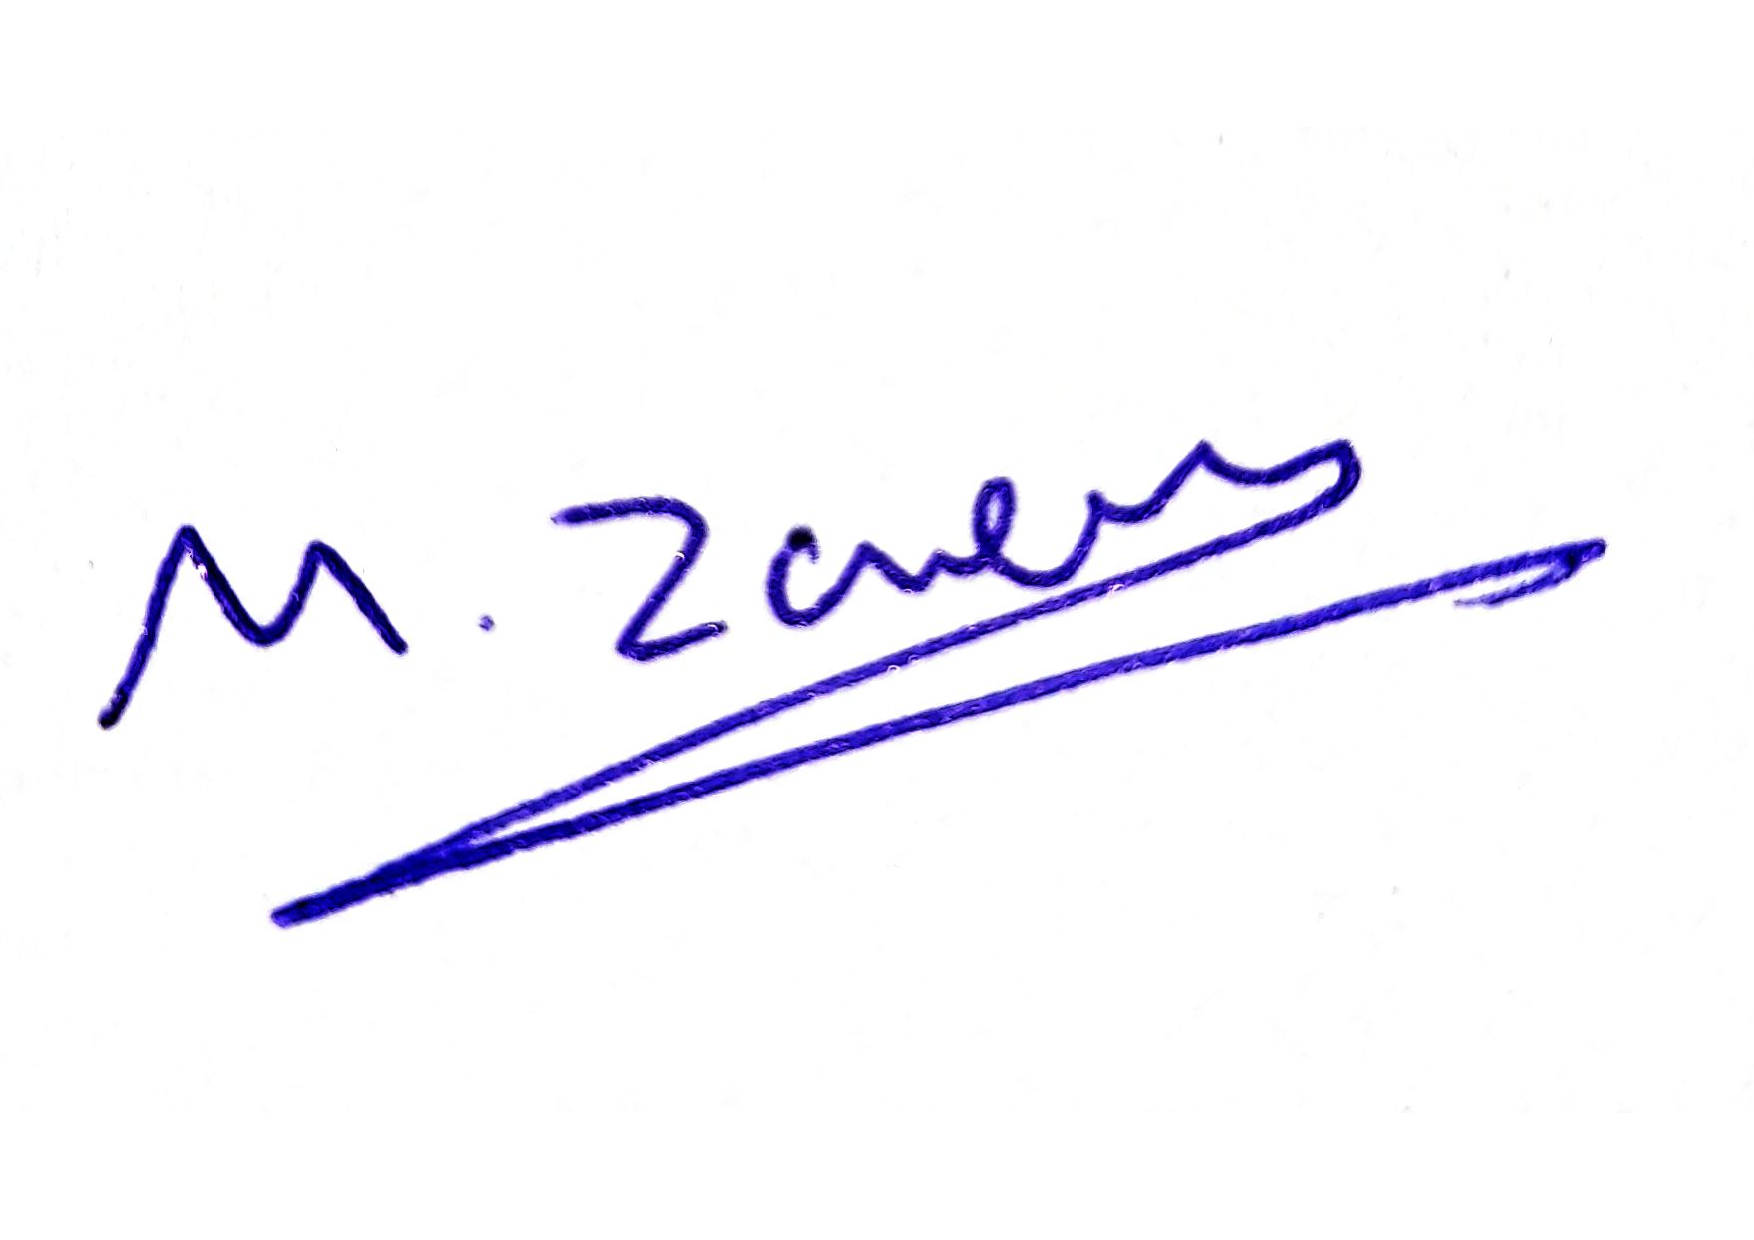
\includegraphics[height=1cm]{Figures/zaeem_sign.pdf}\hspace{0.3cm}}
\\[2ex]
Name: Sheikh Muhammad Fareed
\\[1ex]
Signature: \underline{\hspace{0.3cm}
\includegraphics[height=1cm]{Figures/IMG_5572.jpg.pdf}\hspace{0.3cm}}
\end{flushright}

\vspace{5 cm} %Aatira
 
\hrule %Aatira

\section*{Author's Declaration}
This states Authors’ declaration that the work presented in the report is their own, and has not been submitted/presented previously to any other institution or organization.
\pagebreak

\section*{Abstract}
Colorizing grayscale photographs is an underconstrained problem, and a single model must cover very different kinds of content. This project proposes a region-based Mixture-of-Experts framework for domain-adaptive colorization. Grounded-SAM divides a grayscale image into semantic regions, each region is routed by its text prompt to one of four domain experts (portraits and people, nature and landscapes, urban and man-made scenes, animals), and the expert outputs are merged with soft masks. The experts are fine-tuned copies of DDColor, and a new expert can be added without retraining the others. This report presents the method, the system design, and the plan for evaluating it against general-purpose baselines.
\pagebreak

\section*{Executive Summary}

A grayscale photograph does not contain enough information to determine the original colors of the objects in it, so colorization often has several plausible answers. General-purpose colorization models must handle everything (including people, animals, landscapes, and buildings) with one set of weights, and they are reported to produce desaturated colors, semantic inconsistencies, and color drift between domains.

This project develops a region-based Mixture-of-Experts framework for domain-adaptive colorization. A pretrained open-vocabulary segmentation model, Grounded-SAM, is used to divide a grayscale photograph into semantic regions using predefined text prompts. Each region is cropped with a surrounding margin (20\% by default, adjustable for testing) and routed by its prompt to one of four domain experts: portraits and people, nature and landscapes, urban and man-made scenes, and animals. The experts are fine-tuned copies of the DDColor network with independent weights. They predict only the color channels in the Lab color space, so the brightness and detail of the original photograph are kept unchanged. The outputs are merged with soft mask boundaries to avoid visible seams, and pixels that no region covers are colorized by a fallback expert. A new expert can be added by defining new prompts and training one network. This does not require any modification of the existing pipeline and experts.

The project has five objectives:
\begin{itemize}
    \item identify semantic regions across the four domains;
    \item train a specialized colorization expert for each domain;
    \item route detected regions to the correct expert;
    \item merge the expert outputs with smooth transitions;
    \item demonstrate the addition of a further expert without retraining the existing ones.
\end{itemize}

The system is a pipeline of subsystems (region decomposition, routing, region extraction and expert colorization, and blending) that a central controller calls in order. A basic web interface lets a user upload a grayscale image and view the result. The system is developed iteratively and is expected to be trained and run on free cloud notebook resources, which limits it to a single GPU of moderate memory.

Each stage is measured separately. Segmentation is measured with mean intersection-over-union and routing with routing accuracy. Colorization quality is measured with FID, LPIPS, colorfulness, PSNR, SSIM, and Lab color difference, and seams with the color difference across region boundaries. The framework is compared with three general-purpose baselines (pretrained DDColor-T, DDColor-T fine-tuned on pooled data from all four domains, and pretrained DDColor-L) on single-domain and mixed-scene test sets. Ablations vary the blending, the crop margin, the routing, and the use of segmentation masks, and the extensibility claim is tested by adding a fifth expert.

The project covers still photographs. Video and medical images are outside its scope. The generated colors are plausible interpretations, since historical color accuracy cannot be established from a grayscale image alone. The quality of the result also heavily depends on the quality of outputs produced by the segmentation model(s), because a region that is missed or labeled wrongly is not colorized by the intended expert.

The literature review, the choice of datasets, the methodology, and the system design are complete, and a standalone prototype of the region decomposition stage has been built. The remaining stages are planned for the second phase: routing and region extraction, fine-tuning of the four experts, blending, the web interface, the evaluation against the baselines, and the extensibility demonstration.

The project relates to SDG 11, Target 11.4, the protection of cultural heritage, because colorized versions of historical photographs can supplement the original monochrome records.
\pagebreak


\pagestyle{fancy} %Aatira
\tableofcontents

\pagebreak
\listoffigures	% comment this if there are no figures
\addcontentsline{toc}{chapter}{List of Figures}
\pagebreak
\listoftables % comment this if there are no tables
\addcontentsline{toc}{chapter}{List of Tables}

\mainmatter


\chapter{Introduction}
Image colorization involves assigning plausible colors to grayscale images while preserving their visual structure. It has applications in presenting historical photographs, producing digital media, and supporting visual interpretation \cite{ref21}. However, grayscale images do not contain enough information to determine the original colors of every object. Different colors may have similar brightness values, making colorization an underconstrained problem with several plausible outputs \cite{ref1,ref11}. Existing research identifies this ambiguity as a source of incorrect semantic colors and limited color richness in automatically colorized images \cite{ref1,ref9}.

Recent approaches have explored how semantic understanding and visual context can improve colorization \cite{ref2,ref9,ref11}. DDColor \cite{ref9} combines a pixel decoder with a query-based color decoder to connect spatial features with semantic color representations and reduce color bleeding. Its findings demonstrate the importance of considering both image structure and object meaning when predicting colors. Nevertheless, these findings do not establish that a single model is inherently incapable of handling multiple domains; rather, they motivate further investigation into alternative ways of organizing colorization expertise.

The proposed project, Mixture of Experts Framework for Domain Adaptive Colorization, investigates a region-based alternative. Instead of assigning an entire photograph to one colorization model, the system will identify semantic regions and route them to experts specializing in portraits and people, nature and landscapes, urban and man-made scenes, and animals. The resulting outputs will be combined into a single color image. The project aims to evaluate whether this division of responsibility improves domain-specific color quality and semantic consistency while maintaining coherence across the complete photograph.

\section{Purpose of this Document}
This document outlines the proposed framework for the FYP Development Phase 1 report, establishing a shared understanding among the development team, supervisor, and evaluation panel by detailing the research motivation, objectives, scope, and planned evaluation while distinguishing completed initial study work from pending implementation and experiments. The central research question investigates whether semantic region decomposition combined with domain-specialized colorization experts can enhance color quality and consistency relative to general-purpose colorization approaches. The methodology integrates pretrained Grounded-SAM for region identification, prompt-based routing mechanisms, separately trained domain-specific experts, and a blending module to synthesize results. Evaluation will comprehensively assess segmentation quality, routing accuracy, domain-level colorization performance, boundary consistency, and overall image quality metrics. While the project aims to produce perceptually convincing colorizations, it explicitly acknowledges that historical color authenticity cannot be determined solely from grayscale information.
\section{Intended Audience}
The primary audience for this document comprises the project supervisor and academic evaluation panel, who will assess the project's motivation, feasibility, technical approach, and alignment with its stated objectives, while also supporting the development team by clearly defining the system's boundaries and expected behavior. A secondary audience includes researchers and students interested in image colorization, semantic segmentation, and modular expert-based architectures, as well as practitioners in historical preservation or digital media who may use the document to understand the proposed application and its limitations. Although the document is structured to be accessible, technical knowledge of machine learning and image processing will be helpful for fully interpreting the architecture design and evaluation measures.
\section{Definitions, Acronyms, and Abbreviations}
The following terms are used throughout this document:\\
\textbf{MoE}: Mixture of Experts\\
\textbf{SAM}: Segment Anything Model\\
\textbf{mIoU}: Mean Intersection over Union\\
\textbf{FID}: Frechet Inception Distance\\
\textbf{LPIPS}: Learned Perceptual Image Patch Similarity\\
\textbf{PSNR}: Peak Signal-to-Noise Ratio\\
\textbf{SSIM}: Structural Similarity Index Measure\\
\textbf{SDG}: Sustainable Development Goal
\section{Conclusion}
In conclusion, the proposed Mixture of Experts Framework for Domain-Adaptive Colorization aims to improve grayscale image colorization by using specialized experts instead of relying on a single general-purpose model. The system will divide an image into meaningful regions and assign them to experts for portraits and people, nature and landscapes, urban and man-made scenes, and animals. By combining semantic region decomposition, expert routing, contextual colorization, and output blending, the project aims to generate more plausible and visually coherent color images.
\chapter{Project Vision}
The project envisions a photographic colorization system that combines domain-specific expertise within a single processing framework. A photograph may contain several types of content, and the system will allow different regions to receive different expert treatment. The intended outcome is a working prototype through which the benefits and limitations of this region-based approach can be examined.
\section{Problem Domain Overview}
The project belongs to the domain of automatic image colorization. Its input will be a grayscale photograph, and its output will be a colorized version produced through semantic decomposition, expert routing, specialized processing, and blending. The four initial expert domains are portraits and people, nature and landscapes, urban and man-made scenes, and animals. These domains describe expert responsibilities rather than mutually exclusive categories of complete photographs.

Research on automatic colorization demonstrates the importance of considering multiple plausible colors and the surrounding scene context \cite{ref1,ref11}. Cong et al. \cite{ref11} propose generating reference images that guide colorization and permit localized modifications. Cong et al. Their work supports the relevance of contextual color reasoning, although reference generation and interactive editing are not components of the proposed project. The present framework instead investigates whether separately trained domain experts can provide useful specialization.

For region decomposition, the project will use pretrained Grounded-SAM \cite{ref17} with predefined prompts such as person, animal, building, sky, and vegetation. Grounded-SAM combines Grounding DINO \cite{liu2024groundingdino} with SAM \cite{kirillov2023sam} to support detection and segmentation based on text inputs. This provides a basis for identifying regions associated with the project's expert domains without requiring users to enter prompts manually.

Each identified region will be cropped with an additional boundary whose size will be varied during testing to determine an appropriate value for retaining surrounding context. The cropped region will then be processed by its assigned expert, and soft-mask blending will combine the outputs. In this project, MoE refers to region-level selection among separate colorization networks, rather than token-level routing within a transformer. Together, the related research motivates the use of semantics and context, while the effectiveness of the proposed region--expert combination remains an experimental question.
\section{Problem Statement}
Existing automatic image-colorization methods typically rely on a single model to colorize all types of photographic content. However, general-purpose models are reported to produce desaturated colors \cite{ref1,ref6} and semantic color errors \cite{ref9}, and it remains an open question whether handling visually different domains with one set of weights causes further inconsistencies between them. Developing a unified model that handles these conflicting visual domains remains a recognized challenge. To address this, we are developing a Mixture of Experts framework that routes semantic image regions to domain-specialized colorization experts. The project aims to improve domain-specific color quality and semantic consistency while maintaining coherence across the complete photograph.
\section{Problem Elaboration}
Automatic image colorization must assign plausible colors to diverse visual content despite the absence of explicit chromatic information. Objects with similar grayscale appearances may have different plausible colors, so producing a convincing colorization is not the same as exactly matching a reference image. This ambiguity makes it difficult for a single general-purpose model to handle all types of scenes without encouraging desaturated outputs or semantically inconsistent colors. A photograph may contain people, animals, vegetation, buildings, and other elements simultaneously. The system must identify these regions and associate them with suitable domain-specialized experts. Missed objects, incomplete masks, or ambiguous prompt matches could affect routing and subsequent colorization. Each expert will be trained on whole images from its domain but will receive cropped regions during pipeline operation, with a surrounding boundary intended to retain useful context. Experts operating separately may also make different color decisions for neighboring regions, so soft-mask blending is used to reduce visible seams. The project must assess both local boundary behavior and the quality of the complete output. The framework is further required to support the addition of new experts through extra models and prompt sets without retraining existing ones.
\section{Goals and Objectives}
The overall goal is to develop and evaluate a Mixture of Experts framework that converts grayscale photographs into plausible color images through domain-specialized processing.\\
The specific objectives are:
\begin{itemize}
    \item  Identify semantic regions: Investigate region decomposition across the four selected domains and measure segmentation quality using mIoU on a labeled dataset such as COCO-Stuff \cite{caesar2018cocostuff}.
    \item Develop domain experts: Train a specialized colorization model for each domain. Evaluate held-out outputs using FID, LPIPS, colorfulness, and PSNR/SSIM or Lab color difference against reference images.
    \item Implement expert routing: Assign detected regions to appropriate experts using their semantic characteristics and predefined domain prompts. Measure routing accuracy as the fraction of evaluated regions assigned to the correct expert.
    \item Integrate expert outputs: Combine colorized regions while aiming to preserve smooth transitions and overall visual consistency. Evaluate boundary color differences and compare final-image FID and LPIPS with and without the blending module.
    \item Demonstrate extensibility: Add a further expert and its associated prompt set without modifying or retraining the existing experts.
\end{itemize}
\section{Project Scope}
The project covers the design, development, and evaluation of a working prototype for grayscale photographic colorization. It focuses on four initial domains and supports photographs containing multiple domain types. Its main components are semantic region decomposition, domain-based routing, separately trained colorization experts, contextual cropping, and output blending.\\
The initial study has identified the following candidate datasets:
\begin{itemize}
    \item Portraits and people: CelebA \cite{celeba2015}, CelebA-HQ \cite{pggan2018}, FFHQ \cite{ffhq2019}, DeepFashion-MultiModal \cite{text2human2022}, and COCO \cite{ref19} person images.
    \item Nature and landscapes: Places365 \cite{places365} and SUN397 \cite{sun397}.
    \item Urban and man-made scenes: Cityscapes \cite{ref20}, ADE20K \cite{ref18}, and urban subsets of Places365 \cite{places365}.
    \item Animals: AFHQ \cite{afhq2020}, Oxford-IIIT Pets \cite{pets2012}, and animal subsets of COCO \cite{ref19}.
\end{itemize}
Experts will be trained using color images from their respective domains, with grayscale inputs derived from the L channel in Lab space. This supplies paired training examples without manually annotating colors. A labeled segmentation dataset such as COCO-Stuff \cite{caesar2018cocostuff} will support evaluation of region decomposition.\\
The project deliverables will include:
\begin{itemize}
    \item A working prototype integrating region decomposition, routing, expert inference, and blending.
    \item Four domain-specialized models trained for the initial expert categories.
    \item An experimental evaluation covering the objectives and the effect of blending.
    \item An extensibility demonstration showing incorporation of an additional expert and prompt set.
\end{itemize}
\section{Sustainable Development Goal (SDG)}
The Sustainable Development Goal targeted by this project is Goal 11: Sustainable Cities and Communities. The project relates to Target 11.4, which focuses on protecting and safeguarding cultural and natural heritage. The proposed colorization framework can support the presentation and interpretation of historical grayscale photographs through supplementary colorized versions. This may make historical visual content more accessible and engaging for viewers and researchers. However, the generated colors will represent plausible interpretations, while the original monochrome photographs will remain the primary historical records. The complete SDG list is shown in Figure \ref{fig:1}.
\begin{figure} [!h]
    \centering
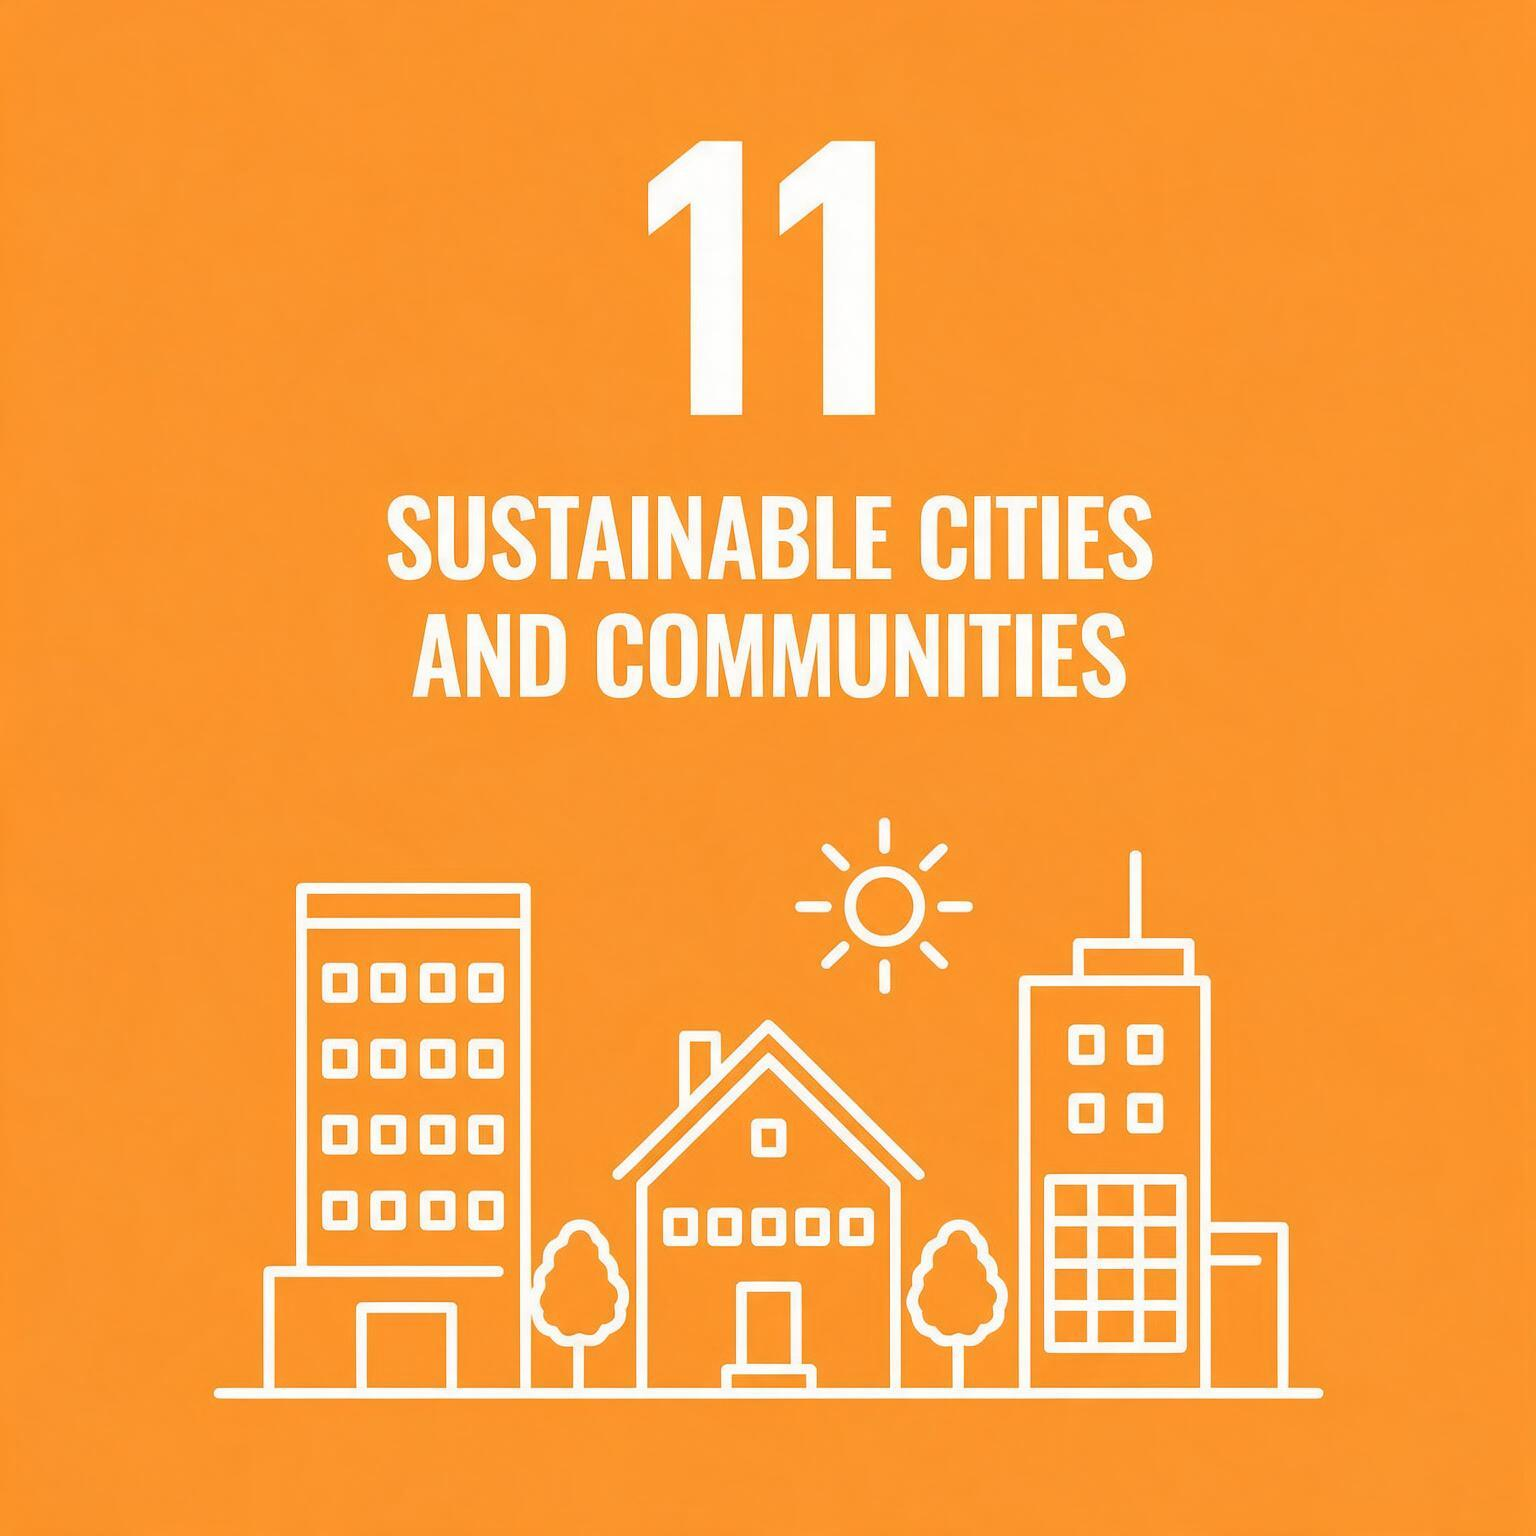
\includegraphics[width=0.7\textwidth]{Figures/Figure-2.1.jpg}
    \caption{Sustainable Cities and Communities.}
                 
    \label{fig:1}
\end{figure}
\chapter{Literature Review / Related Work}
This chapter presents the literature review and related technological work relevant to the proposed Mixture-of-Experts framework for domain-adaptive image colorization. The review covers automatic grayscale-to-color image generation, semantic and contextual colorization, generative and transformer-based approaches, Mixture-of-Experts architectures, and semantic image decomposition. Particular attention is given to the limitations of general-purpose colorization models when processing visually heterogeneous domains. The reviewed literature establishes the technical foundations for decomposing an image into semantically meaningful regions and applying specialized colorization models to those regions.
\section{Definitions, Acronyms, and Abbreviations}
\subsection{Definitions}

\textbf{Image Colorization:} The process of adding suitable colors to a black-and-white (grayscale) image to create a realistic color image.

\textbf{Grayscale Image:} A digital image in which each pixel carries only light intensity or brightness information, containing no color data.

\textbf{Chrominance:} The color-related information of an image, commonly represented separately from luminance in color spaces.

\textbf{Domain:} A visually or semantically coherent category of image content with characteristic color distributions and visual structures.

\textbf{Domain-Specialized Expert:} A colorization model trained primarily on images belonging to a particular visual domain.

\textbf{Mixture of Experts (MoE):} An architecture containing multiple specialized models or expert components together with a mechanism that selects or routes inputs to appropriate experts.

\textbf{Semantic Region:} A spatial region of an image corresponding to an identifiable object, material, or scene component.

\textbf{Routing:} The process of assigning an image region to an appropriate specialized expert.

\textbf{Blending:} The process of combining the outputs of multiple experts into a single image while reducing visible discontinuities between neighboring regions.

\textbf{Color Discontinuity:} A measurable difference in predicted color across the boundary between neighboring regions.

\textbf{Photorealistic Colorization:} Colorization intended to produce visually plausible colors and spatially coherent image appearance.

\textbf{Open-Vocabulary Segmentation:} Semantic detection and segmentation that can use textual descriptions or prompts to identify image regions beyond a fixed closed set of categories.
\subsection{Acronyms}
\textbf{AI:} Artificial Intelligence

\textbf{CNN:} Convolutional Neural Network

\textbf{MoE:} Mixture of Experts

\textbf{GAN:} Generative Adversarial Network

\textbf{ViT:} Vision Transformer

\textbf{FID:} Fréchet Inception Distance

\textbf{LPIPS:} Learned Perceptual Image Patch Similarity

\textbf{PSNR:} Peak Signal-to-Noise Ratio

\textbf{SSIM:} Structural Similarity Index

\textbf{mIoU:} Mean Intersection over Union

\textbf{$\Delta$E:} CIE Lab colour difference

\textbf{Lab:} CIE L*a*b* colour space

\textbf{SAM:} Segment Anything Model

\textbf{RGB:} Red, Green, Blue

\textbf{DINO:} DETR with Improved DeNoising Anchor Boxes / Grounding DINO context

\section{Detailed Literature Review}

The research papers reviewed in this study are divided into four main categories: automatic image colorization, semantic and contextual colorization, Mixture-of-Experts architectures, and semantic segmentation. These reviewed studies provide the technical foundation for analyzing existing approaches and identifying the research gap addressed by the proposed region-routing colorization approach.~

\subsection{Foundations of Automatic Image Colorization}

\subsubsection{Colorful Image Colorization}

Zhang, Isola, and Efros introduced a fully automatic deep-learning approach to grayscale image colorization by treating color prediction as a classification problem rather than straightforward deterministic regression \cite{ref1}. Their approach used a large-scale collection of color images and class rebalancing to address the tendency of colorization models to produce desaturated results. The work demonstrated that the inherent uncertainty of grayscale-to-color mapping should be explicitly considered because multiple plausible colors can correspond to the same luminance information. The authors also introduced a human evaluation in which generated images were compared with ground-truth photographs.

A major strength of this work is that it shows colorization is not a simple task because there can be many possible colors for the same grayscale image. Treating colorization as a prediction problem helped later studies focus on producing more varied and realistic colors. However, it is still a general-purpose model and does not divide the image into different semantic regions or use specialized models for them.

The relationship to the proposed project is important because the proposed system also treats grayscale-to-color mapping as an uncertain prediction task. However, instead of using one general model, it uses multiple specialized experts to handle different image regions. This allows the system to better handle the different types of content found in an image.

\subsubsection{Let There Be Color!: Joint End-to-End Learning of Global and Local Image Priors}

Iizuka, Simo-Serra, and Ishikawa proposed a colorization method that combines global scene information with local image information \cite{ref2}. The method uses the overall scene to help decide suitable colors, while local information helps produce detailed color predictions.

A key strength of this approach is that it combines scene understanding with local color prediction. This is useful because individual pixels usually do not contain enough information to determine their correct color. However, both types of information are handled within one colorization model rather than through separate domain-specific experts.

The proposed framework extends this idea by first identifying meaningful image regions and then including additional context around them. The approximately 20\% (variable to allow for testing) extra region boundary would help preserve surrounding information while allowing specialized experts to process individual regions.

\subsubsection{Real-Time User-Guided Image Colorization with Learned Deep Priors}

Zhang et al. developed a user-guided colorization system where users provide a small number of color hints that are then spread across the image using a CNN-based model \cite{ref3}. Instead of depending only on automatically predicted colors, the system allows users to give local color information to guide the colorization process. The method also suggests possible colors and uses learned semantic information to apply the user\textquotesingle s guidance to relevant areas.

The main strength of this approach is the control it gives to the user. Users can adjust or guide the colors of uncertain regions instead of relying completely on automatic predictions. However, the system depends on user-provided color hints, while the proposed project uses predefined prompts and automatic region decomposition without requiring manual input from the user.

This work is relevant because it shows one way of dealing with uncertainty in image colorization. The proposed framework follows a different approach: instead of relying on the user to handle uncertain regions, it uses semantic routing and domain-specialized experts to deal with differences between image domains.

\subsubsection{Deep Exemplar-Based Colorization}

He et al. proposed a deep exemplar-based method in which a grayscale image is colorized using a separate reference color image \cite{ref4}. The method includes components that measure the similarity between the reference and target images and then use this information to predict and transfer chrominance. The authors also introduced an automatic reference recommendation method based on semantic and luminance information.

The main strength of this approach is the control provided through reference selection. Different reference images can produce different colorization results, giving users more flexibility compared to a fully automatic method. However, the main limitation compared to the proposed project is that it depends on a reference image. It does not divide the target image into different domain-specific regions or process those regions separately using specialized experts.

The proposed project follows a similar idea that different visual contexts may need different color information. However, instead of using an external reference image, the proposed system gets domain-specific knowledge from separately trained experts.

\subsection{Transformer, Generative and Diffusion-Based Colorization}

\subsubsection{Colorization Transformer}

Kumar, Weissenborn, and Kalchbrenner introduced the Colorization Transformer, which applies self-attention to the colorization problem \cite{ref5}. The system first generates a low-resolution coarse colorization and subsequently uses parallel networks to obtain higher-resolution output. The transformer architecture is designed to capture long-range dependencies, allowing information from distant image regions to influence color prediction.

The strength of transformer-based colorization is its ability to model relationships extending beyond local convolutional neighborhoods. The approach also supports multiple colorization samples rather than relying exclusively on one deterministic output. A limitation is that the model remains fundamentally general-purpose rather than explicitly specialized according to semantic domains.

The proposed framework can benefit from this literature when designing individual experts. However, the main architectural distinction is that the proposed system places domain specialization outside the individual colorization model by routing semantic regions to separate experts.

\subsubsection{Towards Vivid and Diverse Image Colorization With Generative Color Prior}

Wu et al. investigated the use of a pretrained GAN as a generative color prior \cite{ref6}. Their approach extracts features representing plausible color distributions and incorporates those features into the colorization process. The resulting method seeks vivid and diverse outputs rather than the desaturated results frequently associated with deterministic prediction.

The approach demonstrates that an explicit generative color prior can improve chromatic richness and diversity. Nevertheless, the color prior is still learned as part of a general colorization framework rather than being explicitly divided according to semantic domains.

The proposed project is related because its objective also includes realistic and perceptually convincing color. The difference is that the proposed project obtains specialization through multiple domain experts rather than through one generalized generative color prior.

\subsubsection{BigColor}

Kim et al. introduced BigColor, a generative color-prior approach intended to improve colorization of complex in-the-wild images \cite{ref7}. The authors specifically identified limitations in previous generative priors that attempted to model both image structure and color simultaneously. BigColor instead focuses its generative prior on color synthesis while preserving spatial structure.

The principal strength is its focus on separating color generation from structural representation. The method supports diverse colorization results and arbitrary input resolutions. Its limitation in relation to the proposed project is that its specialization is still encoded inside a unified generative architecture rather than explicitly assigned by image region.

The proposed project similarly recognizes that image structure and color prediction are closely related, but takes a different architectural route. Semantic decomposition is performed first, after which each region is assigned to an expert whose training data corresponds to a specific domain.

\subsubsection{Palette: Image-to-Image Diffusion Models}

Saharia et al. introduced Palette, a unified conditional diffusion framework for image-to-image translation, including colorization \cite{ref8}. The work evaluates diffusion-based translation on several image restoration and transformation tasks and demonstrates the ability of conditional diffusion models to generate plausible image outputs.

Palette is significant because diffusion provides another mechanism for representing the multiple plausible outputs inherent to image-to-image translation. However, the framework is designed as a general image-to-image model and does not implement the proposed region-level domain-specialized expert architecture.

For the proposed work, Palette demonstrates the importance of multimodal generative modeling but does not resolve the specific problem of conflicting color distributions between different semantic domains within the same photograph.

\subsubsection{DDColor: Towards Photo-Realistic Image Colorization via Dual Decoders}

Kang et al. introduced DDColor, an end-to-end colorization architecture containing a pixel decoder and a query-based color decoder \cite{ref9}. The two components jointly connect multi-scale semantic representations with color queries. The authors specifically address semantic color errors, low color richness, and color bleeding. A colorfulness loss is also used to encourage richer outputs.

DDColor represents a strong general-purpose baseline because it explicitly combines semantic representations with detailed color reconstruction. Its limitation for the proposed project is architectural specialization: it remains a single colorization model rather than a framework where semantically different regions are routed to separate domain experts.

The proposed system can therefore use DDColor-type principles as a conceptual baseline for individual experts, while the principal research contribution remains the region-level MoE architecture. The official implementation also demonstrates that contemporary colorization models can be trained and evaluated as reusable software components \cite{ref10}.

\subsubsection{Automatic Controllable Colorization via Imagination}

Cong et al. proposed an automatic colorization framework that generates candidate reference images through an imagination module and subsequently refines those references before applying them to colorization \cite{ref11}. The system addresses the ambiguity of colorization by generating multiple possible visual references and selecting suitable information for the target.

A significant strength is its support for iterative and localized colorization modifications. It demonstrates that automatically generated semantic references can improve colorization flexibility. Its limitation relative to the proposed work is that the generated references are not organized as independently trained domain experts.

The proposal explicitly cites this work as evidence that grayscale-to-color mapping is multimodal. The proposed framework addresses the same ambiguity from another direction: semantic decomposition and domain-specific specialization rather than generated reference-image selection.

\subsection{Mixture-of-Experts and Conditional Computation}

\subsubsection{Sparsely-Gated Mixture-of-Experts}

Shazeer et al. introduced sparsely gated Mixture-of-Experts layers as a mechanism for increasing model capacity while activating only a subset of expert networks for a particular input \cite{ref12}. A trainable gating network determines which experts participate in processing an input. The work established an important foundation for conditional computation and expert specialization.

The central strength of MoE is the ability to allocate specialized computation to different inputs without requiring every expert to process every input. However, the original application was not image colorization, and its routing mechanism operates at the model/input level rather than according to semantic image regions.

The proposed project adapts the underlying specialization principle to a different problem. Instead of routing complete examples or transformer tokens, the proposed framework routes semantically identified regions to domain-specific colorization experts.

\subsubsection{Switch Transformers}

Fedus, Zoph, and Shazeer developed the Switch Transformer to simplify sparse expert routing and improve the efficiency and stability of large-scale MoE models \cite{ref13}. The architecture routes each token to an expert and thereby separates parameter capacity from the amount of computation performed for every token.

Switch Transformers demonstrate that expert routing can be practical when the routing mechanism is carefully designed. Nevertheless, the architecture is primarily concerned with token-level conditional computation and was not designed for semantic image-region colorization.

The proposed project differs by defining experts according to photographic domains and by performing routing at the level of semantically decomposed regions. This distinction is central to the project\textquotesingle s intended contribution.

\subsubsection{Mixture of a Million Experts}

He proposed PEER, a parameter-efficient expert retrieval mechanism capable of retrieving from a very large pool of small experts using product-key retrieval \cite{ref14}. The work investigates how a large number of small experts can provide increased capacity without activating all parameters simultaneously.

The work strengthens the theoretical motivation for modular expert architectures and shows that fine-grained specialization can be scaled efficiently. However, its experiments concern language-modeling tasks rather than image colorization.

The relevance to the proposed project lies primarily in extensibility. The proposal specifically requires the architecture to support incorporation of new domain experts without rebuilding the entire system or modifying existing experts. The concept of modular expert addition is therefore consistent with broader MoE research.

\subsubsection{Gamma: Toward Generic Image Assessment with Mixture of Assessment Experts}

Zhou et al. introduced Gamma, a mixture-of-assessment-experts framework designed to handle diverse image-assessment tasks and datasets \cite{ref15}. The system uses shared and adaptive experts to capture common and domain-specific information and additionally uses scene-related prompting.

Gamma is especially relevant because it demonstrates that expert specialization can be used to address domain differences within computer vision rather than only in language modeling. Its limitation is that the task is image assessment rather than image generation or colorization.

The proposed project extends the general concept of domain specialization to a generative colorization task. Unlike Gamma, the proposed framework does not use shared/adaptive assessment experts; instead, it trains separate colorization experts for the four domains specified in the proposal.

\subsubsection{RS-MoEGAN: Sparse Mixture-of-Experts for Cross-Modal Remote Sensing Image Generation}

Fan et al. proposed RS-MoEGAN, which applies sparse Mixture-of-Experts routing to cross-modal remote-sensing image generation \cite{ref16}. The motivation is particularly relevant to the proposed project because different land-cover types can impose conflicting requirements on image generation. RS-MoEGAN uses a learned router to assign image tokens to specialized experts.

The work provides direct evidence that MoE can be useful when a generative vision problem contains conflicting domain-specific requirements. Its main limitation relative to the proposed project is the routing granularity and application domain: it uses token-level routing in remote sensing rather than semantic region-level routing for photographic colorization.

The proposed project is closely related conceptually. Both approaches seek to avoid forcing a single generative model to learn conflicting visual mappings. The proposed project differs by decomposing photographic images into semantic regions and routing those regions to four explicitly defined colorization domains.

\subsection{Semantic Region Decomposition and Routing}

\subsubsection{Grounded-SAM}

Ren et al. introduced Grounded-SAM, an assembly of Grounding DINO and the Segment Anything Model that enables open-vocabulary detection and promptable segmentation \cite{ref17}. The system can identify and segment regions according to textual prompts, providing a flexible mechanism for extracting semantically meaningful regions from images.

This capability is particularly suitable for the proposed architecture. The project proposal specifies predefined textual prompts such as person, animal, building, sky, and vegetation and uses the resulting masks to determine which expert should process each region.

A limitation is that Grounded-SAM itself is not a colorization system. Its purpose in the proposed architecture is therefore infrastructural: it supplies the semantic decomposition required by the routing mechanism. The proposed project investigates whether this decomposition can serve as the basis for domain-specialized colorization.

\subsubsection{Instance-Aware Image Colorization}

Su et al. (2020) proposed an instance-aware method for colorizing images containing multiple objects\cite{su2020instance}. A pretrained Mask R-CNN detects objects and provides bounding-box crops. One instance colorization network processes all detected crops, while a separate network processes the full image. The networks have the same architecture but different weights. A learned fusion module combines their intermediate features to predict the final colors.

The authors reported improved PSNR, SSIM, and LPIPS results over the compared methods on ImageNet, COCO-Stuff, and Places205. They also found that directly blending separate object and full-image color predictions produced inconsistencies. This finding highlights the need to evaluate color consistency when combining independently processed regions.

This work is closely related to the proposed project because both use regional processing to produce a complete color image. However, Su et al. use one instance colorization network across object types rather than separate domain experts. The proposed system will use Grounded-SAM masks to identify regions and route them to DDColor-based experts fine-tuned for people, nature, urban scenes, and animals. Their colorized outputs will be combined using soft masks. The project therefore investigates whether domain specialization improves colorization and whether new experts can be added without retraining existing ones. Object-level colorization itself is treated as established prior work.

\subsection{Datasets and Evaluation Foundations}

The proposal identifies several public datasets for constructing domain-specific training sets, including CelebA \cite{celeba2015}, CelebA-HQ \cite{pggan2018}, FFHQ \cite{ffhq2019}, DeepFashion-MultiModal \cite{text2human2022}, COCO \cite{ref19}, Places365 \cite{places365}, SUN397 \cite{sun397}, Cityscapes \cite{ref20}, ADE20K \cite{ref18}, AFHQ \cite{afhq2020}, and Oxford-IIIT Pets \cite{pets2012}. The proposal also specifies that grayscale training inputs are derived from the L channel of Lab-space color images and that COCO-Stuff \cite{caesar2018cocostuff} is used to evaluate region decomposition.

COCO provides object-level annotations and instance segmentations in complex everyday scenes \cite{ref19}, and COCO-Stuff extends these images with pixel-level labels for background classes such as sky, grass, tree, and water \cite{caesar2018cocostuff}. Because it covers both object and background classes, COCO-Stuff is the dataset used to evaluate region decomposition and routing in this project. ADE20K contains dense scene and object annotations and provides a scene-parsing benchmark covering 150 object and stuff categories \cite{ref18}, and Cityscapes provides detailed semantic and instance annotations for urban street scenes \cite{ref20}. Both are relevant to the urban and man-made domain and serve as sources of training images for its expert.

The 2025 survey by Anwar et al. provides an extensive taxonomy of colorization approaches, datasets, metrics, and evaluation protocols \cite{ref21}. It is particularly useful for the proposed project because it confirms the importance of evaluating colorization through multiple complementary measures rather than relying on a single image-quality metric.


\section{Literature Review Summary Table}

\begin{longtable}{|p{2.5cm}|p{4.2cm}|p{4.2cm}|p{3.8cm}|}
\caption{Summary of Relevant Literature}\label{tab:literature-summary}\\
\hline
\textbf{Author} & \textbf{Method} & \textbf{Results} & \textbf{Limitations} \\
\hline
\endhead
\hline
\endlastfoot
Zhang et al. \cite{ref1} & Uses a CNN to predict color classes and gives more importance to rare colors. & Produced brighter colors and achieved a 32\% human fooling rate. & Uses one model for all image content and may assign wrong colors to unclear objects. \\
\hline
Larsson et al. \cite{refLarsson} & Predicts pixel color distributions using basic and semantic image features. & Performed better than earlier automatic colorization methods. & Does not use separate models for different semantic regions. \\
\hline
Iizuka et al. \cite{ref2} & Combines overall scene information with local image features in one CNN. & Produced realistic results across several types of images. & Processes all regions using the same network. \\
\hline
Zhang et al. \cite{ref3} & Uses a CNN and color hints provided by the user. & Produced realistic results in real time with limited user input. & Requires manual guidance for difficult regions. \\
\hline
He et al. \cite{ref4} & Transfers colors from a reference image using learned similarity and color propagation. & Produced customizable results, even with less related reference images. & Requires a suitable reference image and an additional selection process. \\
\hline
Wu et al. \cite{ref6} & Uses color information learned by a pretrained GAN to guide colorization. & Produced vivid and varied colors in a single forward pass. & Uses one general color prior instead of separate domain experts. \\
\hline
Kim et al. \cite{ref7} & Uses a BigGAN inspired network to learn color information while keeping image structure. & Produced different plausible results and supported different image sizes. & Does not send semantic regions to separate experts. \\
\hline
Saharia et al. \cite{ref8} & Uses a conditional diffusion model for colorization and other image tasks. & Performed better than several GAN and regression methods. & It is a general image translation model without region based experts. \\
\hline
Kumar et al. \cite{ref5} & Uses a transformer for initial color prediction followed by networks that increase image resolution. & Produced detailed and varied colorizations with strong FID and human evaluation results. & Uses one transformer model instead of separate domain experts. \\
\hline
Kang et al. \cite{ref9} & Uses a pixel decoder and a color decoder to connect semantic features with color predictions. & Improved color quality and reduced color bleeding. & Remains a single general purpose colorization model. \\
\hline
Cong et al. \cite{ref11} & Generates possible reference images and improves them before colorization. & Allowed local changes and more control over the final colors. & Depends on generated references instead of trained domain experts. \\
\hline
Shazeer et al. \cite{ref12} & Uses a routing network to activate only selected experts for each input. & Increased model capacity without using every expert at the same time. & Was designed mainly for language tasks, not image colorization. \\
\hline
Fedus et al. \cite{ref13} & Routes each token to one expert using a simpler sparse routing method. & Improved training speed while supporting very large models. & Uses token routing for language models rather than image region routing. \\
\hline
He \cite{ref14} & Uses product key retrieval to select experts from a very large expert pool. & Improved the balance between performance and computation in language models. & Does not directly address image colorization or visual region routing. \\
\hline
Zhou et al. \cite{ref15} & Uses shared and specialized experts for different image assessment datasets. & Improved assessment across several image types and datasets. & Focuses on image assessment rather than image generation or colorization. \\
\hline
RS-MoEGAN \cite{ref16} & Uses a router to send image tokens to specialized experts in a Vision Transformer. & Helped handle different visual regions while using only selected experts. & Focuses on remote sensing images rather than normal photograph colorization. \\
\hline
Grounded-SAM \cite{ref17} & Combines text based object detection with the Segment Anything Model. & Produces masks for objects identified through text prompts. & Performs segmentation only and does not colorize images. \\
\hline
Zhou et al. \cite{ref18} & Provides ADE20K images with detailed labels for 150 classes. & Supports the training and evaluation of scene segmentation models. & It is a general segmentation dataset, not a colorization dataset. \\
\hline
Lin et al. \cite{ref19} & Provides COCO images with object and instance segmentation labels. & Contains 328,000 images and about 2.5 million labeled objects. & Was created for object recognition rather than image colorization. \\
\hline
Cordts et al. \cite{ref20} & Provides semantic and instance labels for urban street images. & Contains 5,000 detailed and 20,000 coarse annotations. & Mainly covers urban streets and has limited nonurban content. \\
\hline
Anwar et al. \cite{ref21} & Reviews colorization methods, datasets, training methods, and evaluation measures. & Provides a useful overview and comparison of existing colorization research. & Does not propose a region based Mixture of Experts colorization system. \\
\hline
\end{longtable}


The literature demonstrates three recurring characteristics of modern colorization research. First, grayscale-to-color prediction is inherently ambiguous, motivating probabilistic, generative, or multimodal approaches. Second, semantic and contextual information is essential for preventing incorrect or visually inconsistent colors. Third, MoE research provides a mechanism for separating conflicting knowledge across specialized components.

\section{Related Applications and Existing Development Systems}

\subsection{DDColor}

DDColor is an open source implementation of the ICCV 2023 dual decoder colorization architecture \cite{ref9,ref10}. The project provides pretrained models, training scripts, inference functionality, and model export support.

Its principal strength is the availability of a complete research implementation and a colorization architecture explicitly designed to reduce semantic color errors and color bleeding. Its limitation relative to the proposed project is that the colorization model remains general purpose rather than consisting of separate experts for people, nature, urban and man made scenes, and animals.

\subsection{Colorful Image Colorization}

The Colorful Image Colorization project provides an implementation of the ECCV 2016 colorization method and supports automatic grayscale to color conversion \cite{ref1,ref22}. Its major strength is its simple automatic inference pipeline and established research foundation. Its principal limitation relative to the proposed project is that it applies a general colorization model rather than selecting domain specific experts for different semantic regions.

\subsection{DeOldify}

DeOldify \cite{deoldify} is an open source image and film colorization project intended for the restoration and colorization of historical images and footage. Its documentation describes both image and video colorization and emphasizes improvements in artifacts, detail, and color rendering.

Its principal strength is its practical restoration capability and support for both image and video scenarios. However, video is explicitly outside the current scope of the proposed project, and DeOldify does not implement the proposed four domain semantic routing architecture. The project therefore serves as a practical general purpose comparison rather than an architectural equivalent.

\subsection{DeepAI Image Colorizer}

DeepAI \cite{deepai} provides an accessible image colorization application through which users can upload images and request automatic colorization.

The main advantage of DeepAI Image Colorizer is its accessibility through an application interface, which removes the need for users to train or operate a research model. However, its underlying model architecture and routing strategy are not exposed sufficiently to establish the type of domain specialized processing proposed in this project. Consequently, it is useful as an application level comparison rather than as an architectural baseline.


\subsection{Identification of Research and Technological Gap}

The reviewed literature establishes substantial progress in automatic image colorization. CNN based methods demonstrated practical automatic color prediction, transformer approaches improved long range reasoning, generative priors improved color diversity, diffusion models introduced powerful multimodal image generation, and recent systems such as DDColor improved semantic and perceptual quality.

Nevertheless, the dominant colorization formulation remains based on a single general purpose model. The proposal identifies the underlying issue as the need for one model to approximate color distributions across substantially different visual domains.

Mixture of Experts research provides evidence that conflicting knowledge can be separated among specialized experts. RS-MoEGAN is particularly relevant because it uses expert routing for different visual generation requirements \cite{ref16}, while Gamma demonstrates domain aware experts in image assessment \cite{ref15}.

However, the reviewed literature does not establish a directly equivalent system that combines the following components:

\begin{enumerate}
    \item Semantic region decomposition of a photographic image.
    
    \item Assignment of each region to one of four domain specific colorization experts.
    
    \item Approximately 20\% contextual boundary expansion around each selected region.
    
    \item Independent expert colorization.
    
    \item Soft mask blending of all expert outputs into one image.
    
    \item Addition of new experts through new prompts without modifying or retraining existing experts.
\end{enumerate}

This combination represents the technological gap addressed by the proposed development. The project therefore does not attempt to introduce colorization itself as a new problem. Instead, it investigates whether domain specialization through semantic region level Mixture of Experts routing can improve the handling of heterogeneous photographs compared with a monolithic colorization approach.

\section{Conclusion}

The literature review shows that image colorization has developed from traditional and CNN based methods to transformer, GAN, diffusion, exemplar based, and controllable generative approaches. These developments have improved color richness, semantic consistency, visual quality, and diversity. However, grayscale to color mapping remains uncertain, especially when a single photograph contains several visually different domains.

The reviewed Mixture of Experts research provides another useful approach in which different or conflicting types of knowledge can be handled by specialized experts and selected through a routing mechanism. Semantic segmentation systems such as Grounded-SAM provide a way to identify different image regions according to their visual and semantic characteristics.

The proposed project combines these ideas into a framework for photographic image colorization. It focuses on four domains: people, nature and landscapes, urban and man made scenes, and animals. The framework combines semantic decomposition, domain routing, specialized colorization, contextual region expansion, and soft mask blending. The evaluation framework measures segmentation, routing, individual expert quality, boundary consistency, and final image quality. The final system is intended to be a working prototype that can also support the addition of new experts without requiring the existing architecture to be redesigned.
 
\chapter{Software Requirement Specifications}

This project is a research prototype for testing domain adaptive image colorization with a Mixture of Experts framework. It is different from a normal software application because it does not need user accounts, transactions, or support for many users at the same time. Its main tasks are model training, semantic region detection, expert selection, colorization, blending, and evaluation.

The system also keeps the output of each stage for inspection and debugging purposes. This is necessary because a good final image does not always mean that the segmentation and routing decisions were correct. For this reason, segmentation, routing, expert outputs, and blending will be checked separately before evaluating the complete result.

This chapter explains what the system must do and the conditions under which it will be developed. It covers the main features, functional and nonfunctional requirements, quality attributes, assumptions, hardware and software needs, use cases, data handling, and possible risks.

\section{List of Features}

The main features planned for the prototype are listed below:

\begin{itemize}
    \item Loading grayscale photographs as input.
    
    \item Finding semantic regions with Grounded SAM and predefined text prompts.
    
    \item Dividing detected regions into four domains: people, nature and landscapes, urban and man made scenes, and animals.
    
    \item Extracting each region with approximately 20\% extra surrounding area for context.
    
    \item Sending each region to the expert that matches its domain.
    
    \item Colorizing different regions separately through their assigned experts.
    
    \item Using more than one expert when a photograph contains multiple domains.
    
    \item Joining the colorized regions through soft mask blending.
    
    \item Displaying intermediate outputs such as masks, routing decisions, expert results, and blended images.
    
    \item Measuring performance with segmentation mIoU, routing accuracy, FID, LPIPS, colorfulness, PSNR, SSIM, and Lab color difference where needed.
    
    \item Adding new experts and prompt sets without retraining the existing experts.
\end{itemize}

Together, these features make it possible to build and test region based expert routing for photographic image colorization.

\section{Functional Requirements}

The following requirements describe the main operations of the system. Each one includes a simple result that can be used to confirm that it works.

\begin{longtable}{|p{1.2cm}|p{7.1cm}|p{6.0cm}|}
\caption{Functional Requirements of the Proposed System}
\label{tab:functional-requirements}\\
\hline
\textbf{ID} & \textbf{Requirement} & \textbf{Acceptance Evidence} \\ \hline
\endfirsthead

\hline
\textbf{ID} & \textbf{Requirement} & \textbf{Acceptance Evidence} \\ \hline
\endhead

FR1 &
The system shall take a grayscale photograph as input. &
A valid grayscale image is loaded without an error. \\ \hline

FR2 &
The system shall find semantic regions using predefined prompts and Grounded SAM. &
Masks are produced for the supported regions in the image. \\ \hline

FR3 &
The system shall extract every selected region with approximately 20\% extra surrounding area. &
The crop contains the detected region and some nearby image content. \\ \hline

FR4 &
The system shall assign each region to a suitable domain expert. &
An expert assignment is produced for every selected region. \\ \hline

FR5 &
The system shall colorize each region through its assigned expert. &
Every routed region produces a colorized result. \\ \hline

FR6 &
The system shall allow different experts to process the same photograph. &
An image with multiple domains can produce results from more than one expert. \\ \hline

FR7 &
The system shall combine the expert outputs using soft mask blending. &
The separate expert results are joined into one color image. \\ \hline

FR8 &
The system shall keep every region in its original position during reconstruction. &
Each colorized region appears in the correct place in the final image. \\ \hline

FR9 &
The system shall display each detected region, its assigned expert, and its colorized output during the current session. &
The interface shows the masks, routing decisions, and expert outputs without permanently saving them. \\ \hline

FR10 &
The system shall evaluate segmentation, routing, expert colorization, and the final image. &
The required measurements are calculated and displayed for the evaluated stages. \\ \hline

FR11 &
The system shall allow a new expert and prompt set to be added without retraining existing experts. &
The new expert works while the existing experts remain unchanged. \\ \hline

FR12 &
The system shall send a region to the fallback expert when it cannot be assigned to a suitable domain-specific expert. &
A region with no suitable domain-specific assignment is processed by the fallback expert. \\ \hline

\end{longtable}

The link between a region, its expert, its output, and its location in the photograph must remain clear throughout the pipeline. Otherwise, a wrong routing decision could be hidden after the regions are blended together.

\section{Quality Attributes}

The most important quality goals for this system are correctness, modularity, reproducibility, evaluability, extensibility, and sensible use of hardware resources.

\subsection{Correctness}

Detected regions must stay in the correct position and size when the final image is rebuilt. The system must also keep each region linked to the expert that processed it. No region should be moved, removed, or resized incorrectly during reconstruction.

\subsection{Modularity}

Segmentation, region extraction, routing, colorization, blending, and evaluation should be kept as separate modules. This will make it easier to test or replace one part without changing the rest of the system.

\subsection{Reproducibility}

The project should keep a record of training settings, dataset splits, expert models, prompts, random seeds, and evaluation settings. This will allow the same experiment to be run again under similar conditions.

\subsection{Evaluability}

The system must keep semantic masks, expert assignments, individual expert results, and blended outputs available for inspection. These outputs are needed to judge each stage instead of judging everything from the final image alone.

\subsection{Extensibility}

It should be possible to add a new domain expert and its prompts without retraining the existing models. The routing configuration should clearly show which prompts belong to each expert.

\subsection{Resource Awareness}

The implementation must work within the available GPU memory, RAM, storage, and training time. Early experiments will therefore use smaller images, batches, and datasets before moving to larger settings.

\section{Non-Functional Requirements}

These requirements describe how the prototype should behave during development and experimentation.

\subsection{Performance}

Segmentation, routing, colorization, and blending should finish within a practical amount of time on the available hardware. A strict real time target is not needed because the system is being built for experiments, not live public use.

Image resolution and batch size should be adjustable so that training can be matched to the available computing power.

\subsection{Reusability}

The main components should be written as reusable modules. Shared image processing and evaluation functions should be used by all experts instead of being copied into several files.

\subsection{Maintainability}

Model paths, prompts, dataset locations, and experiment settings should be kept in configuration files rather than hard coded throughout the program. The source code should also be divided into clear and manageable modules.

\subsection{Reliability}

Failures during segmentation, routing, model loading, or colorization should be recorded. The system should not present an incomplete result as successful when one of its main stages has failed.

\subsection{Usability}

The prototype may be run through scripts, configuration files, notebooks, or a basic interface. The steps for selecting an image, loading the models, running the pipeline, and finding the results should be easy to follow.

\subsection{Compatibility}

The system should accept common image formats such as PNG and JPEG. The required versions of Python, the deep learning framework, CUDA, and other libraries should be documented.

\subsection{Scalability}

The first version will contain four experts, but the structure should allow more experts to be added later. Supporting many users at the same time is not part of this project.

\subsection{Concurrent Usage}

The prototype is intended for use by the project team during experiments. For this reason, there is no fixed target for concurrent users, request throughput, or continuous service availability.

\section{Assumptions}

The project is based on the following assumptions:

\begin{itemize}
    \item Suitable image datasets are available for training the first four experts.
    
    \item The datasets contain enough variety for people, nature and landscapes, urban and man made scenes, and animals.
    
    \item Grounded SAM and its pretrained models are available for the experiments.
    
    \item Predefined text prompts can identify the main concepts needed by the four domain setup.
    
    \item Training images can be converted to grayscale by using the L channel of the Lab color space.
    
    \item The original color images are available as references during training and evaluation.
    
    \item A labeled dataset such as ADE20K or COCO is available for testing segmentation.
    
    \item Ground truth color images are available for measurements that need reference images.
    
    \item The first version focuses only on photographic image colorization.
    
    \item Video and medical image colorization are outside the current scope.
    
    \item The initial implementation uses approximately 20\% extra context around each region.
    
    \item The amount of extra context may be tested later if enough time and computing resources are available.
\end{itemize}

These assumptions set the starting conditions for developing and testing the prototype.

\section{Use Cases}

This section presents the main computational scenarios required by the proposed research system. Since the project does not define conventional application users, the actor used in the use cases is the Project Operator or Experimenter. This actor represents the person executing the prototype, configuring experiments, and examining the generated results.

\begin{longtable}{|p{0.7cm}|p{2.7cm}|p{3.5cm}|p{0.8cm}|p{5.7cm}|}
\caption{Use Case for Colorizing a Grayscale Photograph}
\label{tab:uc-colorize-photograph}\\
\hline

\multicolumn{2}{|l|}{\textbf{Name}} &
\multicolumn{3}{p{10.4cm}|}{Colorize Grayscale Photograph} \\ \hline

\multicolumn{2}{|l|}{\textbf{Actors}} &
\multicolumn{3}{p{10.4cm}|}{Project Operator or Experimenter} \\ \hline

\multicolumn{2}{|l|}{\textbf{Summary}} &
\multicolumn{3}{p{10.4cm}|}{
The operator provides a grayscale photograph. The system identifies semantic regions, routes the regions to suitable experts, colorizes the regions, combines the expert outputs, and produces a final color image.
} \\ \hline

\multicolumn{2}{|l|}{\textbf{Pre-Conditions}} &
\multicolumn{3}{p{10.4cm}|}{
The colorization pipeline, Grounded SAM, and the supported domain experts must be available. A valid grayscale photograph must be provided.
} \\ \hline

\multicolumn{2}{|l|}{\textbf{Post-Conditions}} &
\multicolumn{3}{p{10.4cm}|}{
A final colorized image and the corresponding intermediate outputs are produced.
} \\ \hline

\multicolumn{2}{|l|}{\textbf{Special Requirements}} &
\multicolumn{3}{p{10.4cm}|}{
The system must use predefined prompts and should not require manual region selection. Sufficient memory must be available to load the segmentation and expert models.
} \\ \hline

\multicolumn{5}{|c|}{\textbf{Basic Flow}} \\ \hline

\multicolumn{3}{|c|}{\textbf{Actor Action}} &
\multicolumn{2}{c|}{\textbf{System Response}} \\ \hline

1 &
\multicolumn{2}{p{6.2cm}|}{
The operator provides a grayscale photograph.
} &
1 &
The system validates and loads the input image. \\ \hline

2 &
\multicolumn{2}{p{6.2cm}|}{
The operator starts the colorization process.
} &
2 &
The system passes the image to the semantic region decomposition component. \\ \hline

3 &
\multicolumn{2}{p{6.2cm}|}{
The operator waits while semantic decomposition is performed.
} &
3 &
Grounded SAM generates semantic region masks using the predefined prompts. \\ \hline

4 &
\multicolumn{2}{p{6.2cm}|}{
The operator waits while the detected regions are prepared.
} &
4 &
The system extracts each selected region with approximately 20\% additional surrounding context. \\ \hline

5 &
\multicolumn{2}{p{6.2cm}|}{
The operator waits while routing is performed.
} &
5 &
The routing component assigns each region to the appropriate domain expert. \\ \hline

6 &
\multicolumn{2}{p{6.2cm}|}{
The operator waits while the experts process their assigned regions.
} &
6 &
Each selected expert produces a colorized version of its assigned region. \\ \hline

7 &
\multicolumn{2}{p{6.2cm}|}{
The operator waits while reconstruction is completed.
} &
7 &
The blending component combines the expert outputs using soft region boundaries. \\ \hline

8 &
\multicolumn{2}{p{6.2cm}|}{
The operator examines the generated result.
} &
8 &
The system provides the final color image and its intermediate outputs for evaluation. \\ \hline

\multicolumn{5}{|c|}{\textbf{Alternative Flow}} \\ \hline

1A &
\multicolumn{2}{p{6.2cm}|}{
The operator provides an invalid or unsupported image.
} &
1A &
The system rejects the input and displays or records an appropriate error message. \\ \hline

3A &
\multicolumn{2}{p{6.2cm}|}{
No supported semantic region is identified.
} &
3A &
The system sends the whole image to the fallback expert and records that no domain region was found. \\ \hline

5A &
\multicolumn{2}{p{6.2cm}|}{
A region cannot be associated with a supported expert.
} &
5A &
The system sends the region to the fallback expert and records the routing limitation. \\ \hline

6A &
\multicolumn{2}{p{6.2cm}|}{
An expert model fails to process its assigned region.
} &
6A &
The system records the failure and does not present the incomplete result as a successful final output. \\ \hline

\end{longtable}


\begin{longtable}{|p{0.7cm}|p{2.7cm}|p{3.5cm}|p{0.8cm}|p{5.7cm}|}
\caption{Use Case for Adding a New Domain Expert}
\label{tab:uc-add-expert}\\
\hline

\multicolumn{2}{|l|}{\textbf{Name}} &
\multicolumn{3}{p{10.4cm}|}{Add New Domain Expert} \\ \hline

\multicolumn{2}{|l|}{\textbf{Actors}} &
\multicolumn{3}{p{10.4cm}|}{Project Operator or Experimenter} \\ \hline

\multicolumn{2}{|l|}{\textbf{Summary}} &
\multicolumn{3}{p{10.4cm}|}{
The operator adds a new domain expert and its associated prompt set without redesigning the framework or retraining the existing experts.
} \\ \hline

\multicolumn{2}{|l|}{\textbf{Pre-Conditions}} &
\multicolumn{3}{p{10.4cm}|}{
A trained expert model, its configuration, and its corresponding prompt set must be available.
} \\ \hline

\multicolumn{2}{|l|}{\textbf{Post-Conditions}} &
\multicolumn{3}{p{10.4cm}|}{
The new expert becomes available to the routing framework while the existing experts remain unchanged.
} \\ \hline

\multicolumn{2}{|l|}{\textbf{Special Requirements}} &
\multicolumn{3}{p{10.4cm}|}{
Existing expert models must not be retrained or modified when the new expert is added.
} \\ \hline

\multicolumn{5}{|c|}{\textbf{Basic Flow}} \\ \hline

\multicolumn{3}{|c|}{\textbf{Actor Action}} &
\multicolumn{2}{c|}{\textbf{System Response}} \\ \hline

1 &
\multicolumn{2}{p{6.2cm}|}{
The operator prepares a trained expert model and its configuration.
} &
1 &
The system receives and validates the new expert configuration. \\ \hline

2 &
\multicolumn{2}{p{6.2cm}|}{
The operator defines the corresponding textual prompt set.
} &
2 &
The routing configuration associates the new prompts with the new expert. \\ \hline

3 &
\multicolumn{2}{p{6.2cm}|}{
The operator starts the expert registration process.
} &
3 &
The system registers the new expert and its prompt mapping. \\ \hline

4 &
\multicolumn{2}{p{6.2cm}|}{
The operator verifies the existing expert configuration.
} &
4 &
The system keeps all existing experts available without retraining or modification. \\ \hline

5 &
\multicolumn{2}{p{6.2cm}|}{
The operator performs a routing test using an image from the new domain.
} &
5 &
The system routes supported regions from the new domain to the newly added expert. \\ \hline

\multicolumn{5}{|c|}{\textbf{Alternative Flow}} \\ \hline

2A &
\multicolumn{2}{p{6.2cm}|}{
The operator provides an incomplete or invalid prompt configuration.
} &
2A &
The system rejects the configuration and records the validation problem. \\ \hline

3A &
\multicolumn{2}{p{6.2cm}|}{
The new expert is incompatible with the required input or output format.
} &
3A &
The system does not register the expert and reports the compatibility issue. \\ \hline

5A &
\multicolumn{2}{p{6.2cm}|}{
The prompt set does not correctly identify the intended domain.
} &
5A &
The system records or flags the configuration problem instead of routing regions incorrectly. \\ \hline

\end{longtable}

These use cases represent the main operational behavior of the prototype. The first use case covers the complete colorization pipeline, while the second demonstrates the extensibility requirement of the proposed architecture.

\section{Hardware and Software Requirements}

This section describes the hardware and software environment required to develop, train, execute, and evaluate the proposed system.

\subsection{Hardware Requirements}

The project requires access to hardware capable of executing modern deep learning models. GPU acceleration is expected to be important for training the colorization experts and running the segmentation and colorization pipeline efficiently.

The required GPU memory depends on the selected expert architecture, image resolution, and batch size. Exact memory requirements will therefore be determined through initial training experiments rather than assuming a fixed value before implementation.

Adequate system memory and storage are required for maintaining training datasets, model checkpoints, generated outputs, semantic masks, and evaluation results. Smaller training batches or image resolutions may be used if hardware limitations are encountered.

The recommended hardware includes:

\begin{itemize}
    \item A CUDA compatible GPU for training and inference.
    
    \item At least 8 GB of system memory for initial development.
    
    \item Sufficient storage for datasets, model checkpoints, and experimental outputs.
    
    \item A multicore processor for dataset preparation and image processing.
\end{itemize}

Cloud based GPU resources may be used when the available local hardware is insufficient for training or large scale evaluation.

\subsection{Software Requirements}

The project will use Next.js for the frontend and FastAPI for the backend. The model training, image processing, routing, blending, and evaluation components will be implemented in Python. The required software components are:

\begin{itemize}
    \item Next.js for developing the web-based user interface of the system.
    
    \item HTML and CSS for designing and styling the application interface.
    
    \item Node.js and npm for running the Next.js development environment and managing frontend packages.
    
    \item FastAPI for developing the backend APIs and connecting the frontend with the image colorization pipeline.
    
    \item Python for implementing semantic segmentation, expert routing, image colorization, output blending, and evaluation.
    
    \item PyTorch for training and running the domain-specific colorization experts.
    
    \item Grounded SAM and its pretrained components for detecting and segmenting semantic regions within an image.
    
    \item OpenCV and Pillow for image conversion, cropping, resizing, mask processing, boundary expansion, and output blending.
    
    \item NumPy and related scientific computing libraries for numerical and image-processing operations.
    
    \item Evaluation libraries for calculating mIoU, FID, LPIPS, colorfulness, PSNR, SSIM, and Lab color difference.
    
    \item Jupyter Notebook or Google Colab for model training, testing, and recording experimental results.
    
    \item Git and GitHub for source code management and version control.
    
    \item Visual Studio Code as the main development environment.
    
    \item CUDA and compatible GPU drivers for faster model training and inference.
\end{itemize}

The Next.js frontend will allow the user to upload a grayscale image and view the semantic masks, assigned experts, individual expert outputs, and final colorized image. The FastAPI backend will receive the image, run the Python-based colorization pipeline, and return the generated results to the frontend. Model configurations, prompts, dataset splits, and experiment settings will also be stored to support the reproduction of important experiments.
\section{Graphical User Interface}

The proposed project is primarily a research prototype and does not require a complex graphical user interface. The system is operated through a basic web interface built with Next.js, which communicates with the Python pipeline through a FastAPI backend (Section~\ref{sec:architecture}). The pipeline can also be run from scripts and notebooks without the interface, which the evaluation experiments use.

The web interface provides the following functions:

\begin{itemize}
    \item Selection or upload of a grayscale photograph.
    
    \item Initiation of the colorization pipeline.
    
    \item Display of the generated semantic masks.
    
    \item Display of the expert assigned to each region.
    
    \item Display of individual expert outputs.
    
    \item Display and saving of the final blended color image.
    
    \item Display or export of the calculated evaluation results.
\end{itemize}

Figure \ref{fig:prototype-interface} shows the proposed interface of the system.

\begin{figure}[htbp]
    \centering
    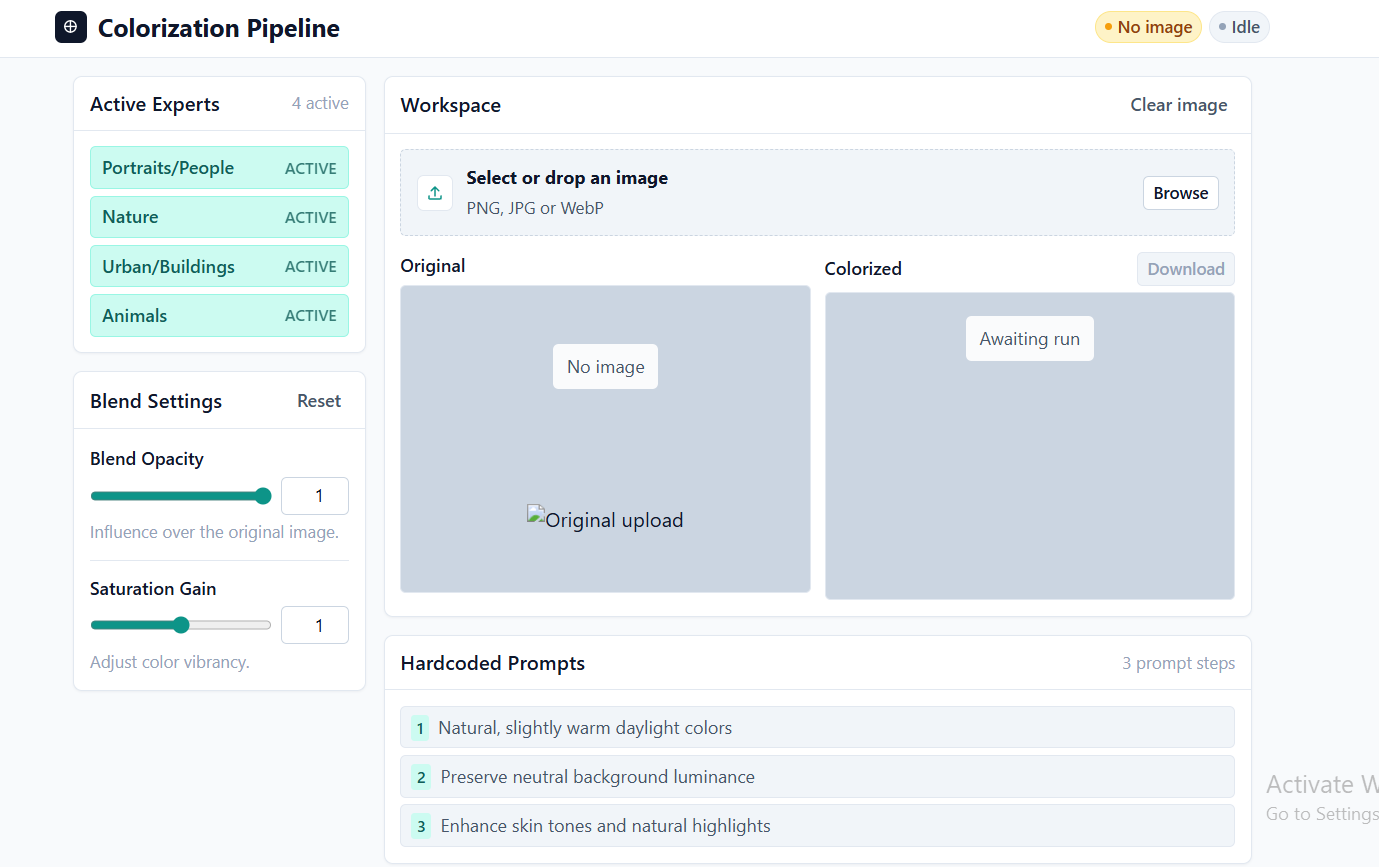
\includegraphics[
        width=0.85\textwidth,
        keepaspectratio
    ]{Figures/Figure-4.8.1.png}
    \caption{Proposed Interface of the Image Colorization System}
    \label{fig:prototype-interface}
\end{figure}

The interface displays the intermediate results because each stage of the system must be evaluated separately. The final colorized image alone is not enough to verify the segmentation and routing results.

\section{Database Design}

The proposed system does not require a conventional relational or NoSQL database. It does not maintain user accounts, transactions, or continuously changing application records. Experimental information can be maintained using directories, configuration files, CSV files, JSON files, and model checkpoint files.

\subsection{ER Diagram}

An ER diagram is not required because the proposed prototype does not use a relational database. The system stores experimental artifacts as files rather than as persistent relational entities.

The logical relationship between the principal experimental artifacts is that one input image may produce multiple semantic regions, each semantic region is assigned to one expert, each expert produces a colorized region, and the colorized regions are combined into one final image.

\subsection{Data Dictionary}

Table \ref{tab:data-dictionary} describes the main data artifacts maintained by the system.

\begin{longtable}{|p{3.2cm}|p{3.0cm}|p{7.4cm}|}
\caption{Data Dictionary for Experimental Artifacts}
\label{tab:data-dictionary}\\
\hline
\textbf{Data Item} & \textbf{Format} & \textbf{Description} \\ \hline
\endfirsthead

\hline
\textbf{Data Item} & \textbf{Format} & \textbf{Description} \\ \hline
\endhead

Input Image &
PNG or JPEG &
The grayscale photograph provided to the colorization pipeline. \\ \hline

Ground Truth Image &
PNG or JPEG &
The original color image used as a reference during training or evaluation. \\ \hline

Semantic Mask &
PNG, tensor, or array &
A mask identifying the pixels associated with a detected semantic region. \\ \hline

Region Label &
Text &
The semantic concept detected using a predefined textual prompt. \\ \hline

Expert Identifier &
Text or integer &
The identifier of the expert assigned to process a semantic region. \\ \hline

Contextual Crop &
Image or tensor &
The selected semantic region together with approximately 20\% additional surrounding context. \\ \hline

Expert Output &
Image or tensor &
The colorized result generated by an individual expert. \\ \hline

Final Output &
PNG or JPEG &
The complete color image generated after soft mask blending. \\ \hline

Prompt Configuration &
JSON, YAML, or text &
The predefined prompts and their associations with the available experts. \\ \hline

Model Configuration &
JSON or YAML &
The architecture, training, and inference settings of an expert model. \\ \hline

Model Checkpoint &
Model file &
The learned parameters of a trained colorization expert. \\ \hline

Evaluation Record &
CSV or JSON &
The segmentation, routing, expert, blending, and final image evaluation results. \\ \hline

\end{longtable}

\section{Risk Analysis}

The proposed system contains several connected components. A failure in an earlier component may affect the later stages of the pipeline. The main technical and project risks are described below.

\subsection{Semantic Segmentation Risk}

Incorrect semantic segmentation may cause image regions to be missed or incorrectly identified. Since routing depends on the generated semantic masks, segmentation errors can affect all remaining stages of the pipeline.

This risk will be monitored using segmentation mIoU and by visually inspecting representative segmentation results.

\subsection{Routing Risk}

Some regions may contain visual characteristics associated with more than one domain. This can make expert selection difficult. Incorrect routing may cause a region to be processed by an unsuitable expert.

Routing accuracy will therefore be evaluated independently using labeled test regions. Uncertain or unsupported regions should also be recorded instead of being assigned silently to an unsuitable expert.

\subsection{Dataset and Expert Training Risk}

The datasets available for the different domains may vary in size, quality, balance, and diversity. This may cause some experts to perform better than others and may make direct comparison difficult.

Domain specific datasets will be prepared separately, and each expert will be evaluated using held out images from its own domain.

\subsection{Blending Risk}

Outputs generated by different experts may contain noticeable color differences near the region boundaries. These differences may produce visible seams when the independently colorized regions are combined.

Contextual region expansion and soft mask blending will be used to reduce this problem. The effectiveness of blending will also be evaluated by comparing results produced with and without the blending component.

\subsection{Computational Risk}

Training multiple experts and running segmentation models may require significant computational resources. Hardware limitations may restrict the training resolution, batch size, dataset size, or number of experiments that can be completed.

Initial experiments will use manageable dataset sizes and training configurations. Larger experiments will only be performed after the resource requirements have been measured.

\subsection{Dependency Risk}

The project depends on external libraries, pretrained models, and frameworks such as Grounded SAM. Changes in library versions or the unavailability of model files may affect implementation and reproducibility.

Required versions and dependencies will be recorded. Important pretrained weights and configuration files should be maintained with the project where their licenses permit local storage.

\subsection{Schedule Risk}

Training, model tuning, and evaluation may require more time than initially expected. Failed experiments may further delay the comparison of the expert models and the complete framework.

Development will be performed incrementally. Initial work will focus on a small but complete pipeline before increasing dataset sizes or introducing additional experiments.

\section{Conclusion}

This chapter defined the requirements of the proposed research oriented image colorization prototype. The main functional requirements cover semantic region decomposition, contextual region extraction, expert routing, domain specific colorization, soft mask blending, evaluation, and expert extensibility.

The quality requirements focus on correctness, modularity, reproducibility, evaluability, maintainability, and resource awareness. The assumptions define the datasets, pretrained components, and scope required for the initial implementation. The hardware and software requirements describe the environment needed to conduct the experiments, while the interface and data organization sections explain how the prototype will be operated and how its experimental outputs will be maintained.

The identified risks demonstrate that the final performance of the system depends on several connected stages. For this reason, segmentation, routing, expert colorization, and blending will be evaluated separately as well as through the final generated image. These requirements provide the foundation for implementing and experimentally evaluating the proposed Mixture of Experts colorization framework.

\chapter{Proposed Approach and Methodology}
\label{ch:method}

This chapter presents the proposed approach as a framework for region-based Mixture-of-Experts (MoE) image colorization. Instead of predicting the colors of an entire photograph with a single network, the framework decomposes a grayscale image into semantic regions, assigns each region to a domain-specialized expert, and merges the expert outputs into one color image. The chapter first gives an overview of the complete pipeline (Section~\ref{sec:framework}) and then describes each stage in turn: region decomposition (Section~\ref{sec:decomposition}), expert routing (Section~\ref{sec:routing}), context-aware region extraction (Section~\ref{sec:extraction}), expert colorization models (Section~\ref{sec:experts}), blending (Section~\ref{sec:blending}), and the procedure for adding new experts (Section~\ref{sec:extensibility}). Section~\ref{sec:evaluation} closes the chapter with the evaluation protocol used to test each objective. The chapter covers the algorithmic and procedural details of the method; the system structure and component interfaces are covered in Chapter~\ref{ch:design}.

\section{Overview of the Proposed Framework}
\label{sec:framework}
The framework takes a grayscale photograph as input and produces a color photograph as output. It treats colorization as a divide-and-conquer problem. A single network must approximate the colors of portraits, landscapes, urban scenes, and animals at the same time, and these domains have different color distributions. The proposed framework therefore assigns each part of the image to a model trained for that kind of content.
\subsection{Pipeline Stages}

The pipeline consists of five stages, shown in
Figure~\ref{fig:pipeline-overview}.

\begin{enumerate}
    \item \textbf{Region decomposition.} Grounded-SAM~\cite{ref17} uses a
          predefined set of text prompts to detect regions and generate
          their masks.

    \item \textbf{Expert routing.} The router uses each detected region's
          label to assign it to one of four domains: portraits and people,
          nature and landscapes, urban and man-made scenes, or animals.
          Pixels left without an owner form the fallback region
          (Section~\ref{sec:fallback}).

    \item \textbf{Context-aware region extraction.} The extractor expands
          each stored bounding box to include nearby context, clips it to
          the image boundaries, and resizes the crop to the expert's input
          size. The default margin adds $20\%$ of the box width on each
          horizontal side and $20\%$ of the box height on each vertical
          side, subject to clipping. The E4 runner applies the same
          cropping procedure to the fallback region
          (Section~\ref{sec:extraction}).

    \item \textbf{Expert colorization.} The assigned expert predicts the
          $a$ and $b$ color channels for each crop. The predictions are
          resized back to the crop dimensions and placed on a canvas at
          the working image resolution.

    \item \textbf{Blending and reconstruction.} The pipeline combines the
          regional and fallback predictions using mask weights. Soft
          masks allow colors to transition gradually where regions meet.
          The blended color channels are then combined with grayscale
          lightness and converted to RGB (Section~\ref{sec:blending}).
\end{enumerate}

In E4, all four domain expert slots and the fallback used the same
pretrained DDColor-T checkpoint. Holding the model weights fixed allowed
the experiment to evaluate the effects of regional processing and blending.

\begin{figure}[H]
    \centering
    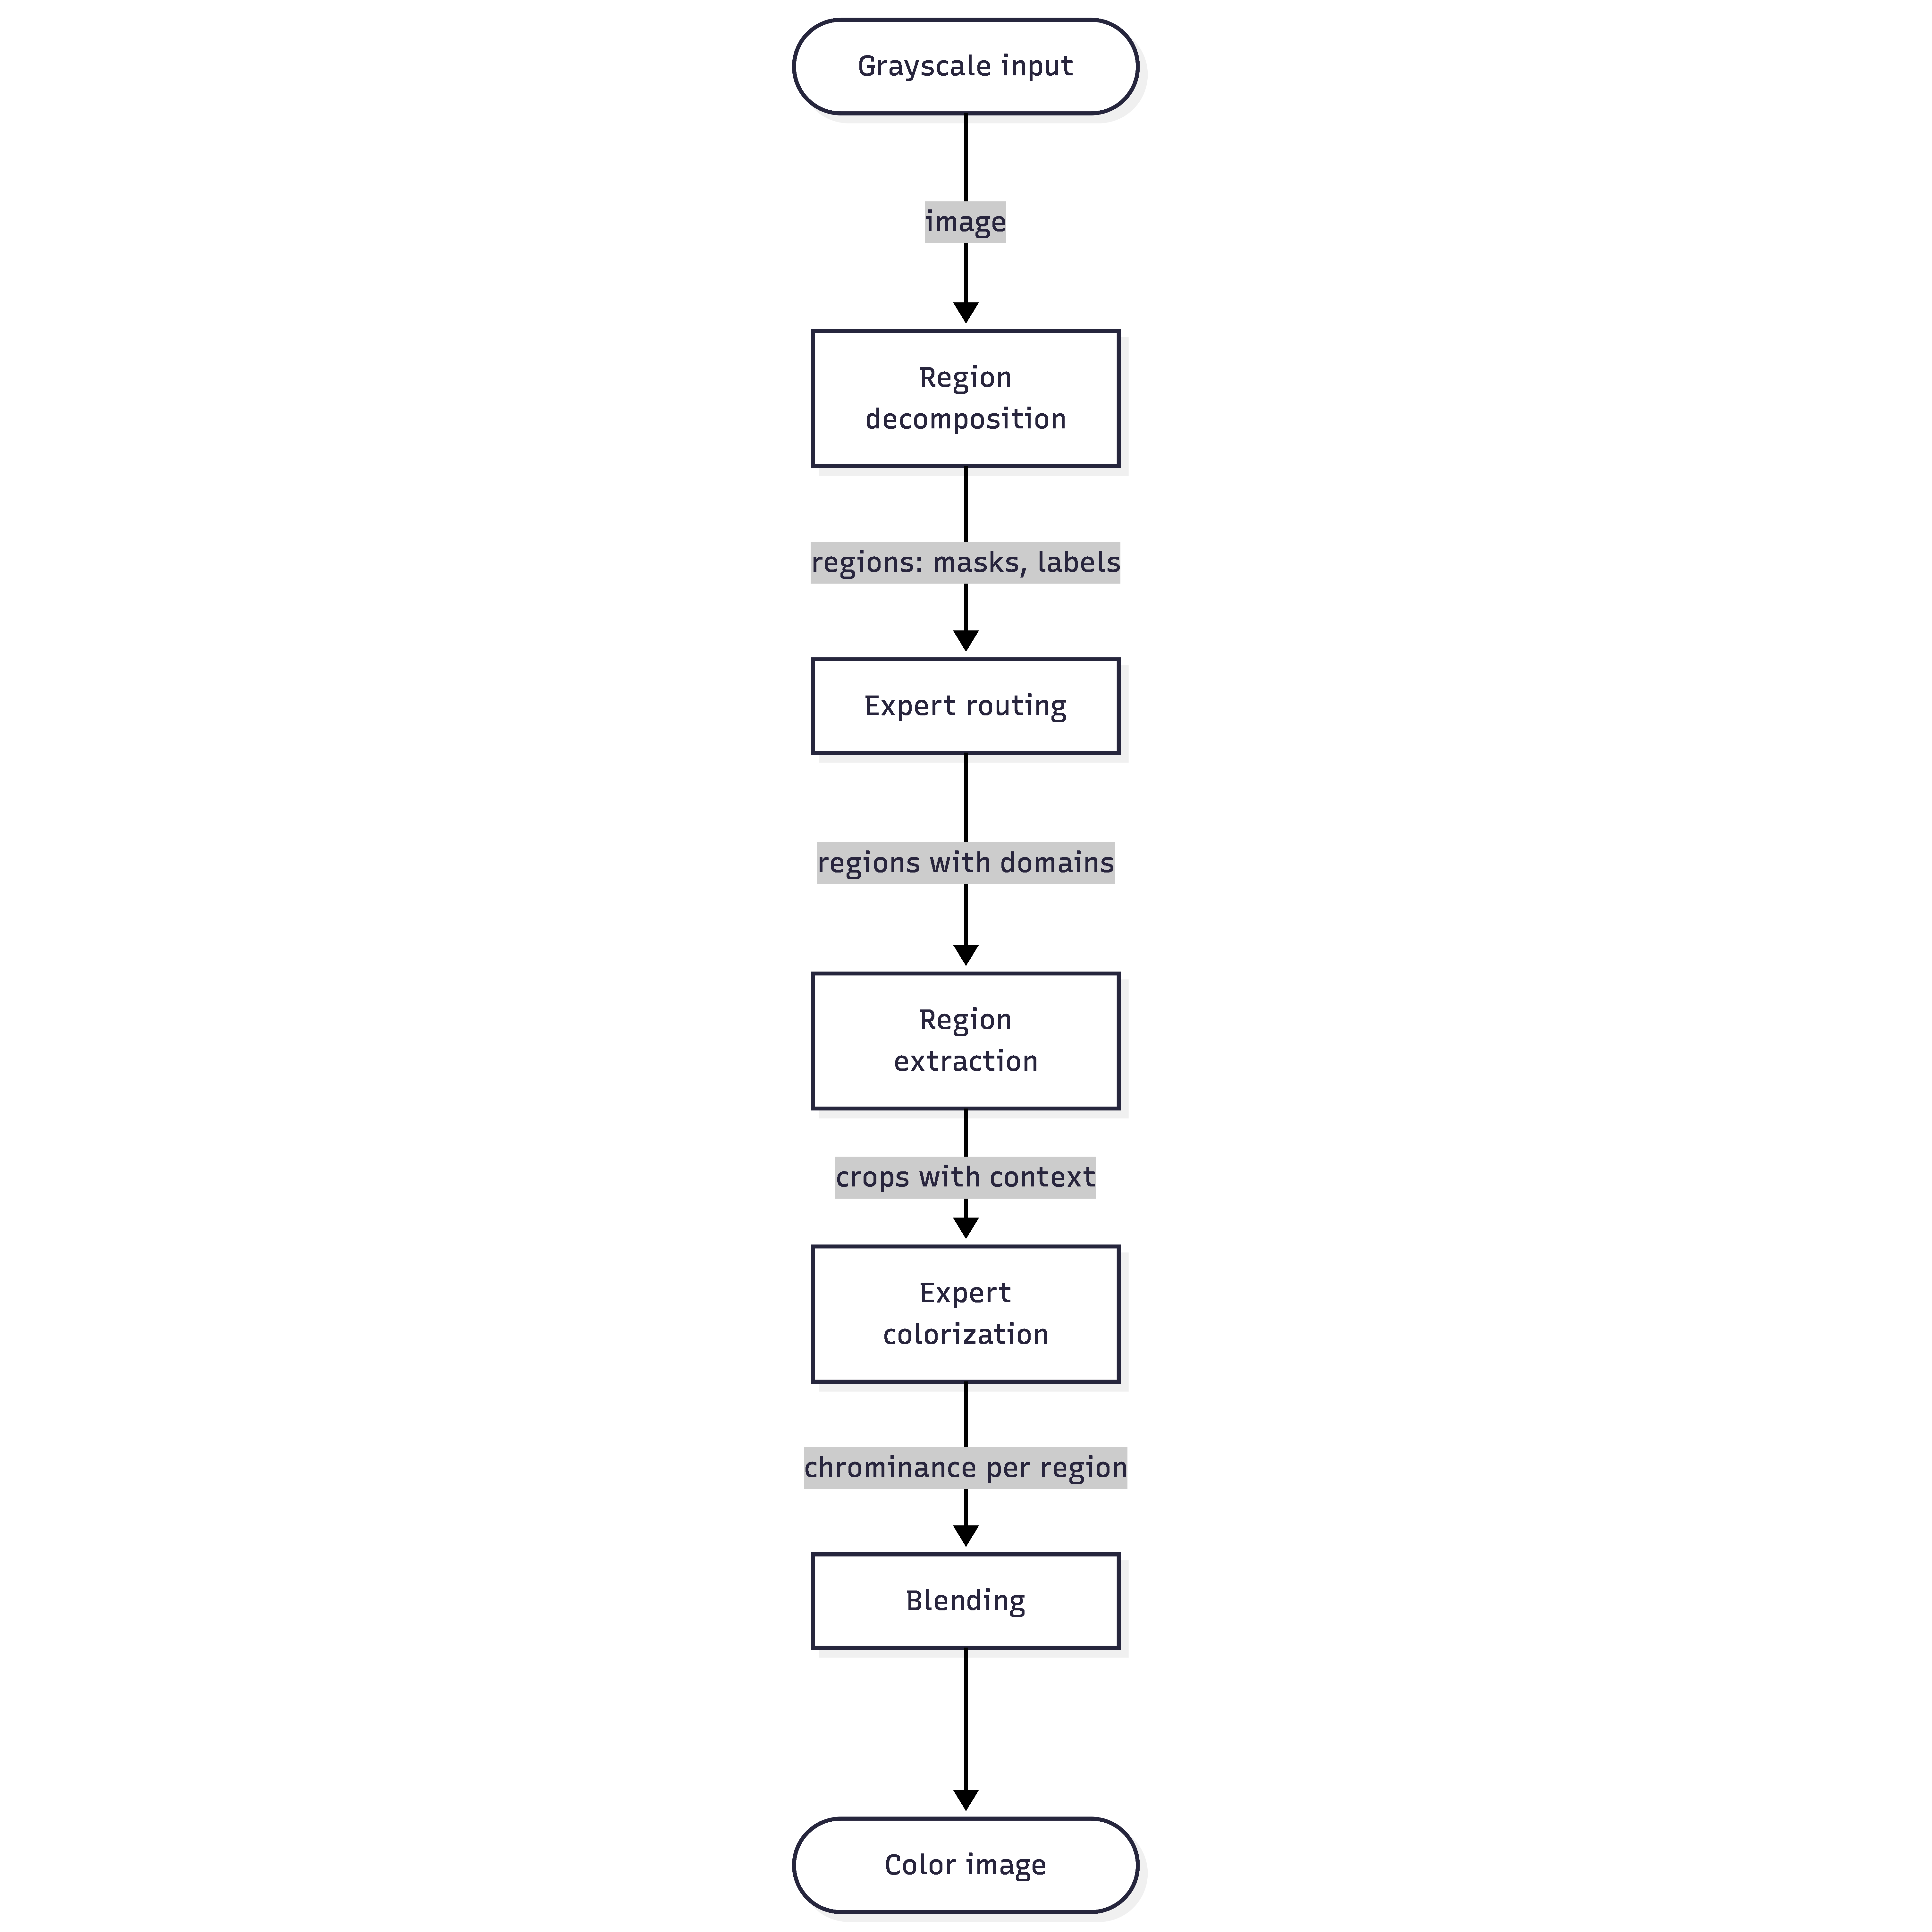
\includegraphics[width=\textwidth]{Figures/pipeline-overview.pdf}
    \caption{Overview of the proposed region-based Mixture-of-Experts colorization pipeline.}
    \label{fig:pipeline-overview}
\end{figure}

\subsection{Color Space and Problem Formulation}
\label{sec:overview}

The framework represents lightness and color separately in the CIE Lab
color space. Let $L\in\mathbb{R}^{H\times W}$ denote the grayscale lightness
at the working image resolution, where $H$ and $W$ are the working image
height and width. In E4, the working grayscale intensities are scaled to
$[0,100]$ and used as $L$. The DDColor-T wrapper converts each resized
neutral Lab crop $(L,0,0)$ to RGB for the network. The network predicts
only the chrominance channels $a$ and $b$.

Let $\widehat{ab}_k(x)$ denote the predicted chrominance from region $k$
mapped back to pixel $x$ of the working image. Each routed region is
associated with expert $E_{d(k)}$, where $d(k)$ is its assigned domain.
Index $k=0$ denotes the fallback, whose binary mask marks pixels with no
owner (Section~\ref{sec:fallback}). Let $M_k(x)$ be the weight from region
$k$ at pixel $x$, and let $D(x)=\sum_{k=0}^{K} M_k(x)$ be the total weight.
The blended chrominance is
\begin{equation}
    \widehat{ab}(x)=
    \begin{cases}
        \displaystyle
        \frac{\sum_{k=0}^{K} M_k(x)\,\widehat{ab}_k(x)}{D(x)},
        & D(x)>0,\\[6pt]
        (0,0), & D(x)=0.
    \end{cases}
\end{equation}
Where multiple predictions contribute, their weights determine how much
each contributes to the result. Pixels with zero total weight receive
neutral chrominance.

If the working image was downscaled, E4 resizes the blended chrominance
and the working grayscale lightness to the original image dimensions.
It then combines them in Lab and converts the result to RGB
(Section~\ref{sec:blending}).
\subsection{Relation to Existing MoE Approaches}

Existing MoE work applies the idea at other levels. RS-MoEGAN~\cite{ref16} routes tokens inside a Vision Transformer, Gamma~\cite{ref15} uses shared and adaptive experts to handle dataset-level biases, and the product-key approach of He~\cite{ref14} scales to a very large number of small experts. In contrast, the proposed framework performs routing at the level of image regions, using a pretrained segmentation model as the router. As a result, no router needs to be trained, each expert only needs to learn a single domain, and a new expert can be added by defining a new prompt set (Section~\ref{sec:extensibility}).

\section{Region Decomposition}
\label{sec:decomposition}

The first stage of the pipeline splits the grayscale input into semantically coherent regions. Region quality directly limits the final result, since a region that is missed, merged with a neighbor, or cut incorrectly is colorized by the wrong expert or with the wrong context. For this reason the decomposition stage is the component examined most closely in the evaluation (Section~\ref{sec:evaluation}).

\subsection{Segmentation Model}

Region decomposition uses Grounded-SAM~\cite{ref17}, which combines two pretrained models. An open-vocabulary detector (Grounding DINO~\cite{liu2024groundingdino}) takes an image and a text prompt and returns bounding boxes for the objects the prompt names. A promptable segmentation model (the Segment Anything Model, SAM~\cite{kirillov2023sam}) then takes each box and returns a pixel-level mask. Both models are used as released, without fine-tuning. Because the detector accepts free-form text, the set of recognizable regions is defined by the prompt list and not by a fixed label set, which is what allows new experts to be added without changing the segmentation model (Section~\ref{sec:extensibility}).



\subsection{Domain Prompt Set}

Each expert domain has a predefined list of text prompts built into the system, so no manual input is required from the user. Table~\ref{tab:prompts} gives the initial prompt set. The set is a starting point and is refined during development by checking which prompts produce reliable masks on the evaluation data.

\begin{table}[htbp]
    \centering
    \caption{Initial prompt set for each expert domain.}
    \label{tab:prompts}
    \begin{tabular}{p{4cm}p{9cm}}
        \hline
        \textbf{Domain} & \textbf{Prompts} \\
        \hline
        Portraits and people & person, face \\
        Nature and landscapes & sky, vegetation, tree\\
        Urban and man-made scenes & building \\
        Animals & animal\\
        \hline
    \end{tabular}
\end{table}

\subsection{Procedure}

For an input image the decomposition stage proceeds as follows.

\begin{enumerate}
    \item Load and resize. The stored image is read as a single-channel grayscale image. If its longer side exceeds 1024 pixels, it is downscaled to that size with Lanczos resampling, keeping the aspect ratio. This limit keeps the memory use of the two models within the available GPU.
    \item Build the text prompt. The class prompts of the domain prompt set are joined into a single lowercase string, with entries separated by a period and the string ending in a period. Grounding DINO receives this string once per image, so all classes are searched for in a single forward pass.
    \item Detect regions. Grounding DINO returns a bounding box in pixel coordinates, a confidence score, and a text label for each detection. A detection is kept only if its box confidence exceeds the box threshold and its match to a word in the prompt exceeds the text threshold.
    \item Filter detections. Detections whose score is below the minimum score are discarded. Duplicate boxes are then removed with per-class non-maximum suppression. Boxes are visited in order of decreasing score, and any remaining box with the same label whose intersection-over-union (IoU) with the visited box exceeds the suppression threshold is removed. Suppression is applied only within a class, so overlapping boxes with different labels are both retained.
    \item Segment each region. The Segment Anything Model encodes the image once. Each retained box is then passed to it as a box prompt, and the model returns a single binary mask for that box. Because the box fixes where the object is, the segmentation model only refines the object boundary and does not search for objects itself.
    \item Merge fragments of the same object. Masks are visited in order of decreasing area. For each mask not yet merged, every other unmerged mask with the same label is absorbed if its containment exceeds the merge threshold, where containment is the area of the intersection divided by the area of the candidate mask. The absorbed mask is combined with the group by union, the group keeps the highest score among its members, and its bounding box is recomputed from the merged mask. The merge decision uses containment: the fraction of a smaller mask that lies inside a larger mask of the same label. A small fragment that lies almost entirely inside a larger mask has a containment close to one and is merged into it, even though it covers only a small part of the larger mask. Two separate instances of the same class, such as two people, overlap very little, so their containment is low and they remain separate regions.
    \item Output. The stage returns a list of regions. Each region holds a binary mask, a label (the prompt that produced it), a confidence score, and a bounding box. The routing stage uses the label (Section~\ref{sec:routing}) and the extraction stage uses the bounding box (Section~\ref{sec:extraction}).
\end{enumerate}

The stage has six parameters: the maximum image side, the box threshold, the text threshold, the minimum detection score, the suppression threshold, and the merge threshold. The maximum image side is fixed at 1024 pixels as a memory limit. The other five are selected on a tuning split of COCO-Stuff: a fixed random subset of 200 images from the official training split, not used for any reported result. The search is a single pass over the parameters, one at a time: each parameter is varied over a small grid while the others remain at their current best value, and the value with the highest mIoU is kept, with ties broken by the higher coverage. The grids are 0.25 to 0.45 in steps of 0.05 for the box threshold, 0.20, 0.25, and 0.30 for the text threshold, 0.30, 0.35, and 0.45 for the minimum score, 0.40, 0.50, and 0.60 for the suppression threshold, and 0.50, 0.60, and 0.70 for the merge threshold. The selected values are 0.25, 0.30, 0.30, 0.50, and 0.50, respectively. The resulting decomposition is compared against the ground-truth labels of the tuning split, and the parameters are then fixed before the segmentation test set (Section~\ref{sec:evaluation}) is used.

\subsection{Limitations of the Decomposition Stage}

Three situations require handling after segmentation. Different prompts can produce overlapping masks for the same object (for example, \textit{person} and \textit{face}). Pixels covered by no mask need a defined fallback. A detection can also be wrong, either by naming the wrong object or by missing one. The rules for overlapping masks and uncovered pixels are part of the routing stage and are described in Section~\ref{sec:routing}. The effect of detection errors on the final image is measured with the routing and end-to-end metrics in Section~\ref{sec:evaluation}.

\section{Expert Routing}
\label{sec:routing}

After decomposition, each region must be assigned to the expert that will colorize it. Routing in the proposed framework is a fixed lookup from the region label to a domain. No router network is trained, so the assignment is deterministic and the only learned components are the experts themselves. A consequence is that routing quality depends on the detector and on the mapping together, and this combined quality is what the routing accuracy metric in Section~\ref{sec:evaluation} measures.

\subsection{Label-to-Domain Mapping}

Every prompt in the domain prompt set belongs to exactly one domain, so the label of a region (the prompt that produced it) determines its expert. Table~\ref{tab:routing} gives the mapping for the prompt set used in the prototype. Extending the framework to a new domain adds rows to this table (Section~\ref{sec:extensibility}).

\begin{table}[htbp]
    \centering
    \renewcommand{\arraystretch}{1.3}
    \caption{Mapping from region labels to domain experts.}
    \label{tab:routing}
    \begin{tabular}{|p{3.5cm}|p{6cm}|}
        \hline
        \textbf{Label} & \textbf{Domain expert} \\
        \hline
        person & Portraits and people \\
        \hline
        face & Portraits and people \\
        \hline
        sky & Nature and landscapes \\
        \hline
        vegetation & Nature and landscapes \\
        \hline
        tree & Nature and landscapes \\
        \hline
        building & Urban and man-made scenes \\
        \hline
        animal & Animals \\
        \hline
    \end{tabular}
\end{table}

A detection whose label does not match exactly one entry of the prompt set cannot be routed and is discarded. Its pixels are then treated as uncovered (Section~\ref{sec:fallback}).

\subsection{Handling Overlapping Regions}
\label{sec:overlap}

Regions with different labels can overlap, for example a person standing in front of a building, or a tree against the sky. Regions with the same label that overlap are already merged during decomposition (Section~\ref{sec:decomposition}). For the remaining overlaps, each contested pixel is assigned to a single region so that its color comes from one expert.

The rule is that a pixel belongs to the smallest region that contains it. Writing $|M_k|$ for the area of mask $M_k$, the owner of pixel $x$ is
\begin{equation}
    k^{*}(x) = \underset{k:\,M_k(x)=1}{\arg\min}\; |M_k|,
\end{equation}
with ties broken by the higher detection score. Smaller regions are usually objects in front of a larger background, so this rule gives the foreground object priority over the surface behind it. The rule uses only mask areas and not the labels, so it applies unchanged when new experts are added. After ownership is assigned, each mask is reduced to the pixels it owns, which makes the masks disjoint. Soft boundaries are then created from these disjoint masks in the blending stage (Section~\ref{sec:blending}).

\subsection{Handling Uncovered Pixels}
\label{sec:fallback}

Some pixels belong to no region because no prompt matched them, a detection was
filtered out, or its label could not be routed. The fallback is represented as
region $k=0$. Its binary mask contains the pixels with no owner after routing,
and its expert uses the pretrained DDColor-T checkpoint.

The fallback therefore runs whenever at least one pixel is uncovered. In the E1
test set this was true for all 500 images, so in practice every image receives
some fallback colorization. At 0.427 coverage, the fallback handled 0.573 of the
evaluated pixels, so the share of each image colorized by the domain experts
depends on coverage as much as on routing (Section~\ref{sec:evaluation}).

In E4, the runner draws a bounding box around the uncovered pixels and applies
the same contextual cropping procedure used for routed regions. If no regions
are routed, the fallback mask and crop cover the whole working image. The runner
computes a fallback prediction for each tested crop margin, even when the
fallback mask is empty. An empty mask is assigned a whole-image box.

In mask mode, the fallback contributes through its uncovered-pixel mask.
Soft blending can extend its contribution into neighboring pixels within the
crop. The fallback prediction is included as $k=0$ in the weighted combination
in Section~\ref{sec:blending}.

\section{Context-Aware Region Extraction}
\label{sec:extraction}

Each routed region is prepared as input for its assigned expert. The extractor
takes a crop around the region, resizes it to the expert's input size, and
maps the predicted colors back to the crop's position in the working image.

\subsection{Cropping with Boundary Context}

Let $(x_0,y_0,x_1,y_1)$ be the bounding box recorded by decomposition, with
width $w=x_1-x_0$ and height $h=y_1-y_0$. For a margin fraction $\rho\geq 0$,
the requested crop before clipping and rounding is
\begin{equation}
    [x_0-\rho w,\,x_1+\rho w]\times[y_0-\rho h,\,y_1+\rho h].
\end{equation}
The extractor clips the coordinates to the working image before rounding
them to the nearest integer, with ties rounded to even. The upper indices
are excluded when slicing, and each crop dimension is at least one pixel.
Extraction uses the stored box even when overlap resolution changes the
pixels owned by a region. In E4, the fallback is cropped by the same
procedure (Section~\ref{sec:fallback}).

The default $\rho=0.2$ requests a margin of $20\%$ of the box width on the
left and right and $20\%$ of the box height on the top and bottom. A larger
margin gives the expert more context and makes the region occupy a smaller
share of the fixed-size network input. The margin also affects the effective
smoothing width (Section~\ref{sec:blending}). Its effect is evaluated in the
margin ablation described in Section~\ref{sec:evaluation}.

\subsection{Input Resizing and Mask Handling}

The extractor resizes the lightness of each rectangular crop to $S\times S$
using bicubic interpolation, where $S$ is the expert's input size. The
expert predicts the chrominance at that size.

The expert sees the entire crop, including its margin, so it can use
neighboring pixels as context. The region mask is applied during
reconstruction, after the prediction has been mapped back to the working
image (Section~\ref{sec:placement}). When soft blending is enabled, the
mask becomes a weight map that can also let the prediction contribute near
the region boundary within the crop.

\subsection{Mapping Expert Outputs Back to the Image}
\label{sec:placement}

The predicted chrominance is resized from $S\times S$ back to the crop's
dimensions using bicubic interpolation. The extractor writes it into a canvas
at the working image resolution, using the stored crop coordinates. The
canvas is zero outside the crop, where the expert has no prediction. All
coordinates refer to the image after the size limit in
Section~\ref{sec:decomposition} has been applied. The blending stage receives
the prediction canvases, the region masks and the crop coordinates.

\section{Expert Colorization Models}
\label{sec:experts}

The framework defines one colorization expert slot for each of the four
domains. The proposed training phase will fine-tune the four experts
independently on domain-specific data. In E4, all four slots and the fallback
used the same pretrained DDColor-T checkpoint. Holding the weights fixed
allowed E4 to evaluate the effects of regional processing and reconstruction.

\subsection{Base Architecture}

All expert slots use DDColor~\cite{ref9}. Its backbone encoder extracts
multi-scale features from the grayscale input, and its pixel decoder
restores spatial resolution. Its color decoder uses a transformer with
learnable color queries that attend to the image features. The outputs of
the two decoders are fused to predict the $a$ and $b$ channels of the Lab
color space, following the formulation in Section~\ref{sec:overview}.

The framework uses DDColor-T with a ConvNeXt-T backbone and 55.0 million
parameters~\cite{ref9,ref10}. The four proposed independently fine-tuned
models would total approximately 220 million parameters. This is close to
the 227.9 million parameters of the largest published variant, allowing
a future comparison with one generalist of similar size
(Section~\ref{sec:evaluation}). Each expert will start from the same
pretrained checkpoint and will be fine-tuned independently, allowing a
checkpoint to be replaced on its own (Section~\ref{sec:extensibility}).
A frozen backbone with domain-specific adapters was also considered for its
lower storage cost. The chosen design gives each expert independent weights.

The experts operate at a fixed square input size $S$. E4 uses $S=256$.
Section~\ref{sec:extraction} describes how crops are resized to this size.

\subsection{Training Data}

Each expert will be trained on whole color images from its own domain.
The training procedure will derive grayscale inputs from the $L$ channel
in Lab and use the $a$ and $b$ channels as targets. This provides
input-target pairs directly from the color images. Table~\ref{tab:datasets}
lists the candidate datasets for each domain.

\begin{table}[htbp]
    \centering
    \caption{Candidate training datasets for each expert domain.}
    \label{tab:datasets}
    \begin{tabular}{p{4.2cm}p{9cm}}
        \hline
        \textbf{Domain} & \textbf{Datasets} \\
        \hline
        Portraits and people & CelebA~\cite{celeba2015}, CelebA-HQ~\cite{pggan2018}, FFHQ~\cite{ffhq2019} (faces); DeepFashion-MultiModal~\cite{text2human2022}, COCO~\cite{ref19} person images (full body) \\
        Nature and landscapes & Places365~\cite{places365}, SUN397~\cite{sun397} \\
        Urban and man-made scenes & Cityscapes~\cite{ref20}, ADE20K~\cite{ref18}, urban subsets of Places365~\cite{places365} \\
        Animals & AFHQ~\cite{afhq2020}, Oxford-IIIT Pets~\cite{pets2012}, animal subsets of COCO~\cite{ref19} \\
        \hline
    \end{tabular}
\end{table}

For datasets that cover several scene types (Places365, SUN397, ADE20K,
and COCO), the training set for each expert will use images or categories
that belong to its domain. The data for each domain will be split into
training, validation, and test sets. The test images will be held out
until evaluation (Section~\ref{sec:evaluation}). Face datasets provide
consistent portrait subjects, and full-body datasets cover the larger
and more varied people regions that decomposition can produce.

\subsection{Training Procedure}
\label{sec:training}

Each expert will be fine-tuned from the pretrained DDColor-T checkpoint
using the released DDColor training code and the training images for its
domain (Table~\ref{tab:datasets}). Training images will be converted to
Lab and resized to $S\times S$. The $L$ channel will provide the lightness
input and the $a$ and $b$ channels will provide the chrominance targets.

Fine-tuning will use the original objective, which combines pixel-level,
perceptual, adversarial, and colorfulness losses. The four experts will be
fine-tuned separately with identical settings so that the training data
are the main difference between them. Validation images will be used to
monitor training and select checkpoints. Test images will be reserved for
final evaluation. The fine-tuning settings will be reported with the
corresponding training results. The fallback will continue to use the
released pretrained checkpoint.

\subsection{Inference Procedure}

At inference time, the wrapper forms a neutral Lab image $(L,0,0)$ from
the resized crop and converts it to RGB for DDColor-T. The wrapper returns
the predicted $a$ and $b$ channels at size $S\times S$. The extractor maps
them back to the working image as described in Section~\ref{sec:placement}.
In E4, the fallback uses the same checkpoint and receives the contextual
crop described in Section~\ref{sec:fallback}.

\section{Blending}
\label{sec:blending}

The extractor produces a chrominance prediction for each crop
(Section~\ref{sec:placement}). Blending combines these predictions at
the working resolution using the region masks as weights. The resulting
chrominance is then combined with grayscale lightness to form the output
image. Soft weights allow predictions to transition gradually where
regions meet.

\subsection{Soft Mask Construction}

Let $B_k\in\{0,1\}^{H\times W}$ be the binary mask supplied for region $k$,
with $k=0$ denoting the fallback. Overlap resolution assigns one owner per
pixel (Section~\ref{sec:overlap}). In E4, fresh decomposition can supply
overlapping SAM-derived masks, while loading a saved decomposition
rebuilds disjoint masks from the ownership map.

The blender applies Gaussian filtering to the mask patch inside crop
$C_k$ and places the result on the working-image canvas. Writing
$\mathcal{G}^{C_k}_{\sigma_k}$ for Gaussian filtering within the crop,
the weight at pixel $x$ is
\begin{equation}
    M_k(x)=
    \begin{cases}
        \mathcal{G}^{C_k}_{\sigma_k}\bigl(B_k|_{C_k}\bigr)(x), & x\in C_k,\\
        0, & x\notin C_k.
    \end{cases}
\end{equation}
Let $w_k^C$ and $h_k^C$ be the final crop width and height after margin
expansion, clipping, and rounding. The effective smoothing width is
\begin{equation}
    \sigma_k =
    \min\!\left(\sigma_0,\,\frac{\rho\min(w_k^C,h_k^C)}{3}\right),
\end{equation}
where $\sigma_0$ defaults to $10$ pixels at the working resolution. When
$\sigma_k=0$ or blending is disabled, the blender uses the binary mask
restricted to the crop. Thus $\rho=0$ also disables Gaussian smoothing.

In the bounding-box ablation, the runner replaces each region mask with
a filled rectangle from its stored box before margin expansion. This also
applies to the fallback. The variant keeps soft blending.

\subsection{Weighted Chrominance Combination}

Let $\widehat{ab}_k(x)$ be the predicted chrominance from region $k$ at
pixel $x$ on the working-image canvas, and let $D(x)=\sum_{k=0}^{K}M_k(x)$
be the total weight at that pixel. The combined chrominance is
\begin{equation}
    \widehat{ab}(x)=
    \begin{cases}
        \displaystyle\frac{\sum_{k=0}^{K} M_k(x)\,\widehat{ab}_k(x)}{D(x)},
        & D(x)>0,\\[6pt]
        (0,0), & D(x)=0.
    \end{cases}
\end{equation}
If only one region has a positive weight, its prediction is used. If
several regions contribute, their predictions are averaged according to
their weights. With smoothing disabled, overlapping binary masks give
equal weight to the contributing predictions. A pixel with zero total
weight receives neutral chrominance.

\subsection{Recombination with Grayscale Lightness}

The blended chrominance has the working image dimensions, which can be
smaller than the original dimensions (Section~\ref{sec:decomposition}).
E4 reconstructs the output at the original dimensions as follows.

\begin{enumerate}
    \item If the input was downscaled, resize $\widehat{ab}$ to the
          original width and height using bilinear interpolation.
    \item Use the working grayscale intensities, scaled to $[0,100]$,
          as the lightness channel $L$. If enlargement is needed, convert
          working $L$ to 8-bit grayscale, resize it with Pillow bicubic
          interpolation, and scale it back to $[0,100]$.
    \item Combine $L$ and $\widehat{ab}$ in Lab, convert the result to RGB,
          and clip and convert the RGB values to 8-bit form.
\end{enumerate}

The grayscale lightness is supplied before RGB conversion. The evaluation
compares the reported boundary color differences and image quality metrics
with and without smoothing (Section~\ref{sec:evaluation}).

\section{Extensibility: Adding a New Expert}
\label{sec:extensibility}

The framework is designed so that a new domain can be added without redesigning the system or retraining the existing experts. Two properties of the design make this possible. Routing is a lookup from region label to domain (Section~\ref{sec:routing}), so there is no router to retrain. Blending uses fixed filters with no learned parameters (Section~\ref{sec:blending}), so there is nothing to retrain there either. The only learned component that a new domain requires is the new expert itself.

\subsection{Procedure for Adding an Expert}

A new expert is added in four steps.

\begin{enumerate}
    \item Define the domain and its prompts: A set of text prompts is chosen for the objects and surfaces that the new expert should handle. Each prompt must belong to exactly one domain, so a new prompt must not duplicate or closely overlap an existing one (Section~\ref{sec:routing}).
    \item Collect training data: Whole color images of the new domain are gathered from public datasets and split into training, validation, and test images, in the same way as for the existing domains (Section~\ref{sec:experts}).
    \item Train the expert: A new copy of the pretrained DDColor-T checkpoint is fine-tuned on the data of the new domain with the training procedure of Section~\ref{sec:training}. No existing expert takes part in this training.
    \item Register the expert: The new prompts are added to the prompt set, the corresponding rows are added to the label-to-domain mapping (Table~\ref{tab:routing}), and an entry giving the location of the new checkpoint is added to the expert registry, a configuration file that maps each domain to its checkpoint file. The registry stores only file locations. A checkpoint is loaded only when a region is routed to its expert (Section~\ref{sec:experts}), so registering a new expert neither loads nor alters the weights of any existing expert.
\end{enumerate}

The first and last steps are changes to configuration and do not alter the decomposition models, the overlap rule, the fallback, or the blending. The segmentation models are used as released, so the new prompts need no additional segmentation training.

\subsection{Independence of Existing Experts}

The weights of each expert are stored in a separate checkpoint, and no parameters are shared between experts (Section~\ref{sec:experts}). Adding an expert therefore leaves the checkpoints of the existing experts untouched, and this can be verified directly by comparing checksums of the checkpoint files before and after the addition.

Two indirect effects on the existing domains remain possible, and neither involves a change to an expert. First, all prompts are given to the detector as one text string (Section~\ref{sec:decomposition}), so adding prompts changes that string, which may change the detections obtained for the existing prompts. Second, regions of the new domain can overlap regions of existing domains, and the overlap rule (Section~\ref{sec:overlap}) can then assign some pixels to a different owner than before. Both effects are measured in the extensibility test (Section~\ref{sec:evaluation}), by comparing the regions and the final colorization of images from the existing domains before and after the new expert is added.

% Preamble: set the fifth-expert domain once, for example \newcommand{\newdomain}{food}
\newcommand{\newdomain}{[new domain]}

\section{Evaluation Protocol}
\label{sec:evaluation}

This section describes how each objective of the project is tested. It defines the datasets and splits, the metrics, the baselines that the framework is compared with, the ablations that isolate the contribution of its components, and the test of extensibility.

\subsection{Datasets and Splits}

Four kinds of test data are used.

\begin{itemize}
    \item Domain test sets: For each expert domain, the held-out test images of the domain datasets (Table~\ref{tab:datasets}). They are used to evaluate each expert on its own domain.
    \item Region-crop test sets: The region crops that the pipeline produces from the domain test images, using the decomposition and extraction stages. They are used to measure how the experts perform on the inputs they receive at inference, as opposed to whole images (Section~\ref{sec:training}).
    \item Segmentation tuning and test sets: The segmentation dataset is COCO-Stuff. The tuning split is a fixed random subset of 200 images from the official train2017 split (seed 42), and the test set is a fixed random subset of 500 images from the official val2017 split (seed 43). The two lists of image identifiers are stored and are disjoint. The tuning split is used only to select the decomposition parameters (Section~\ref{sec:decomposition}); the test set is evaluated only after all parameters are fixed and is used to evaluate region decomposition and routing.
    \item Mixed-scene test set: Images that contain regions from at least two domains (for example a person in an urban scene), selected from the segmentation test set using its annotations.
\end{itemize}

The ground truth for colorization is the original color image, and the grayscale input is its $L$ channel. Test images are never used for training or for choosing parameters. The decomposition parameters are chosen on the segmentation tuning split. The smoothing width $\sigma_0$ and the boundary fraction $\rho$ are chosen on the validation images of the domain datasets. Where two datasets contain the same image, the duplicate is removed from the training data before the test images are fixed.

\subsection{Region Decomposition Metrics}

The quality of decomposition is measured with the mean intersection-over-union (mIoU) on COCO-Stuff~\cite{caesar2018cocostuff}, which provides both object (thing) and background (stuff) classes, such as sky, grass, tree, water, and road, for the same images. Plain COCO instance annotations contain only object classes and cannot evaluate the nature and urban prompts. Each ground-truth class is mapped to the prompt label that covers it. The \textit{animal} prompt covers all of the animal classes of the dataset (for example dog, cat, bird, horse, and cow), and prompts that name closely related categories, such as \textit{vegetation} and \textit{tree}, are evaluated together as one group. The prompt \textit{face} is evaluated as part of the person group, since COCO-Stuff has no face class. Classes without a matching prompt are ignored. Table~\ref{tab:a_groups} lists the COCO-Stuff classes that make up each scoring group.

\begin{table}[htbp]
\centering
\caption{Ground-truth groups used for scoring decomposition and routing.}
\label{tab:a_groups}
\begin{tabular}{|l|l|p{7.5cm}|}
\hline
\textbf{Group} & \textbf{Domain} & \textbf{COCO-Stuff classes} \\ \hline
person & People & person \\ \hline
animal & Animals & bird, cat, dog, horse, sheep, cow, elephant, bear, zebra, giraffe \\ \hline
sky & Nature & sky-other, clouds \\ \hline
vegetation & Nature & tree, grass, bush, plant-other, flower, leaves, branch \\ \hline
building & Urban & building-other, house, roof, skyscraper \\ \hline
\end{tabular}
\end{table}

Every pixel of a test image is given a predicted group, which is the group of the label of the region that owns it after overlap resolution (Section~\ref{sec:overlap}), or an \textit{uncovered} label if no region owns it. The IoU of each group is computed between the predicted and ground-truth label maps, and mIoU is the mean over the groups. Intersection and union are accumulated in a single confusion matrix over the whole test set, so mIoU is not an average of per-image IoU values. Pixels that no region covers count as missed pixels (false negatives) of their true group and are not counted as false positives of any group. Ground-truth maps are resized to the working resolution with nearest-neighbour interpolation before scoring. The result is reported for each group, for each domain (by merging the groups of a domain), and overall. Coverage is reported as the pooled fraction of all test pixels that are owned by some region, not as the mean of the per-image coverage values, and the pooled definition is used whenever a single coverage value is quoted. This fraction determines how much of an image is colorized by the fallback expert rather than a domain expert.

\subsection{Expert Colorization Metrics}
\label{sec:expert-metrics}
Each expert is evaluated on the test set of its own domain, with the following metrics.

\begin{itemize}
    \item FID~\cite{heusel2017fid}: the distance between the feature distributions of the colorized images and the original color images. Lower is better. FID is unreliable on small sets, so the test sets must contain enough images for a stable estimate, and the number of images is reported with each value.
    \item LPIPS~\cite{zhang2018lpips}: a learned perceptual distance between each colorized image and its ground truth. Lower is better.
    \item Colorfulness~\cite{hasler2003colorfulness}: a measure of how saturated and varied the colors of an image are, computed without a reference. It is reported next to the other metrics to detect outputs that are desaturated, which is a typical failure of colorization models.
    \item PSNR and SSIM: pixel-level and structural similarity to the ground truth. Because the luminance of the output equals that of the input, differences come from color only.
    \item $\Delta E$: the mean Euclidean distance in the Lab color space between the output and the ground truth. As the luminance is identical, this is the error in the chrominance channels.
\end{itemize}

A grayscale photograph has many plausible colorings, so similarity to the one original coloring (PSNR, SSIM, $\Delta E$) penalizes plausible alternatives. These metrics are therefore read together with FID, LPIPS, and colorfulness and not alone. Each expert is evaluated on the whole-image test set and on the region-crop test set, and the difference between the two shows how much the use of whole images in training affects the results on crops.

\subsection{Routing Accuracy}

Routing accuracy is the fraction of regions that are assigned to the correct expert. For each region produced on the segmentation test set, the region's pixels are the pixels it owns after overlap resolution (Section~\ref{sec:overlap}), not its raw segmentation mask. The ground-truth class that covers the largest share of these pixels is found, and ties between classes are resolved in favour of the class with the lowest class number. The domain of that class is taken from the class-to-domain mapping. A region is routed correctly if its assigned domain equals this domain. Regions whose dominant class belongs to no domain are excluded from the accuracy and counted separately; regions that contain no labeled pixel are also excluded and counted separately (41 routed regions in the E1/E2 test set). The accuracy is reported overall and for each domain, with a confusion matrix between domains. Since routing is a lookup from the label (Section~\ref{sec:routing}), this metric measures the combined correctness of the detector's labels and of the mapping.
\subsection{Blending Metrics}

E4 compares the default soft-blending configuration with a variant that
disables Gaussian smoothing. Both variants use the same normalized
combination of regional predictions. When smoothing is disabled, the
blender uses binary masks restricted to their crops. If two binary masks
overlap, their predictions are averaged at the overlapping pixels.

The comparison uses the same 100 images for every condition. The E4
results include boundary $\Delta E$, Lab $\Delta E$, LPIPS, PSNR, SSIM,
and colorfulness. Boundary $\Delta E$ is reported as the boundary score
recorded by the experiment. The available run records leave unverified
whether the score subtracts the natural color change in the ground-truth
image or uses the same boundary locations across all variants. FID was
part of the proposed evaluation protocol and is unreported for E4.

\subsection{Baselines and Ablations}

E4 compares the regional pipeline with pretrained DDColor-T applied to
the whole image on the same 100 inputs. All four domain expert slots and
the fallback in the regional pipeline use the same pretrained DDColor-T
checkpoint. This comparison therefore measures the effects of regional
processing and reconstruction with the model weights held fixed.

The broader evaluation protocol includes two additional comparisons:

\begin{enumerate}
    \item \textbf{DDColor-T fine-tuned on pooled data.} A single model
          will be fine-tuned on the combined training images from the
          four domains. Comparing it with independently fine-tuned
          domain experts will help separate the effect of specialization
          from the effect of fine-tuning.

    \item \textbf{Pretrained DDColor-L applied to the whole image.}
          This model provides a separate generalist comparison. Its
          227.9 million parameters are close to the approximately
          220 million parameters of the four proposed domain experts.
\end{enumerate}

Table~\ref{tab:ablations} lists the settings tested in E4. The reference
configuration uses region masks, soft blending, a crop margin of
$\rho=0.2$, and a base smoothing width of $\sigma_0=10$ pixels.
Each ablation changes one configuration setting. Changing $\rho$
affects both the context available to the model and the cap on the
effective smoothing width (Section~\ref{sec:blending}).

\begin{table}[htbp]
    \centering
    \caption{Ablations evaluated in E4.}
    \label{tab:ablations}
    \begin{tabular}{p{4.0cm}p{8.5cm}}
        \hline
        \textbf{Component} & \textbf{Variants} \\
        \hline
        Blending &
        Soft masks or binary masks without Gaussian smoothing \\

        Base smoothing width $\sigma_0$ &
        $2$, $5$, $10$, $15$, and $20$ pixels at the working resolution \\

        Crop margin $\rho$ &
        $0$, $0.1$, $0.2$, and $0.3$ per side \\

        Region shape &
        Region masks or filled bounding boxes, with soft blending
        enabled in both variants \\
        \hline
    \end{tabular}
\end{table}

The shuffled-routing ablation is planned for the evaluation with
independently fine-tuned experts. It will assign each routed region to
a randomly selected incorrect domain expert and compare the resulting
image with the image produced by the normal routing assignments.

\subsection{Extensibility Test}

The extensibility claim is tested by adding a fifth expert for the domain Vehicles, following the procedure of Section~\ref{sec:extensibility}. The test checks three things.

\begin{itemize}
    \item Existing experts are unchanged: The checksums of the four existing checkpoints are compared before and after the addition.
    \item The new expert works: It is evaluated on the test set of its domain with the metrics of Section~\ref{sec:expert-metrics}, against the baselines above.
    \item Existing domains are not degraded: For images from the four existing domains, the regions found by the decomposition stage and the final results are compared before and after the addition. The change in the regions is measured by the IoU between the masks before and after, and the change in the results by the difference in FID and LPIPS. Any difference can arise only from the changed prompt string and from the overlap rule (Section~\ref{sec:extensibility}), and the test reports its size.
\end{itemize}

The files and configuration entries that had to be changed to add the expert are also recorded, to document how much of the system was left untouched.

\section*{Conclusion}

This chapter described a region-based Mixture-of-Experts framework for image colorization. A pretrained open-vocabulary segmentation model decomposes the grayscale input into regions, each region is routed to an expert by a lookup from its label, and the experts, which are fine-tuned copies of DDColor-T with independent weights, predict the chrominance of the crops they receive. The outputs are merged with soft masks and combined with the original luminance, so that the detail of the input is preserved. A new expert is added by defining new prompts and training one new network, without modifying the existing ones. The evaluation protocol tests each of these claims against baselines and ablations. The next chapter presents the architecture of the system and the design of its components.

\chapter{High-Level and Low-Level Design}
\label{ch:design}
This chapter presents the design of the system that realizes the method described in Chapter~\ref{ch:method}. It begins with an overview of the system and its basic design approach (Section~\ref{sec:sysoverview}). It then states the assumptions, constraints, and goals that shaped the design (Section~\ref{sec:considerations}). The architecture is described next, from the top-level components down to the subsystems and their interactions (Section~\ref{sec:architecture}), followed by the strategies behind the main design decisions (Section~\ref{sec:strategies}). The low-level design is given as a class diagram with descriptions of its classes (Section~\ref{sec:classdiagram}), and the chapter closes with the policies and tactics that govern implementation details such as configuration, testing, and source organization (Section~\ref{sec:policies}).

\section{System Overview}
\label{sec:sysoverview}

\subsection{Purpose and Functionality}

The system converts a grayscale photograph into a color image. It is the working prototype of the region-based Mixture-of-Experts colorization framework proposed in this project. Instead of colorizing the whole image with one network, the system divides the image into semantic regions, colorizes each region with an expert trained for its domain, and merges the results into one image.

At run time, the system performs the following functions:

\begin{itemize}
    \item Region decomposition: detects and segments the regions of the image that belong to the supported domains.
    \item Expert routing: assigns each region to a domain expert, resolves overlaps between regions, and provides a fallback for pixels that belong to no region.
    \item Region extraction: cuts each region out together with its surrounding context and prepares it as input for its expert.
    \item Expert colorization: predicts the chrominance of each region with the assigned expert.
    \item Blending and reconstruction: merges the per-region predictions with soft masks and combines the result with the original luminance to form the output image.
    \item User interaction: lets the user upload a grayscale photograph through a basic web interface and view the colorized result.
\end{itemize}

Two further functions take place outside this path. The experts are trained offline on domain datasets, and the system as a whole is evaluated against baselines with the metrics of Section~\ref{sec:evaluation}. The system is also designed so that a new expert can be added as an extension (Section~\ref{sec:extensibility}).

The scope of the system is photographic colorization of still images. It does not provide manual control over the colors of individual objects, and extension to video and medical imagery is outside the present work.

\subsection{Basic Design Approach}

The system is organized as a pipeline of stages, and each stage is implemented as a subsystem with a defined input and output. A stage receives the output of the previous stage and does not depend on how that output was produced. This keeps the stages separable, so that each one can be tested on its own and replaced without changes to the others. Table~\ref{tab:stagemap} relates the stages of the method in Chapter~\ref{ch:method} to the subsystems of the design.

\begin{table}[htbp]
    \centering
    \caption{Relation between the stages of the method (Chapter~\ref{ch:method}) and the subsystems of the design.}
    \label{tab:stagemap}
    \begin{tabular}{p{4.6cm}p{3.4cm}p{5cm}}
        \hline
        \textbf{Stage} & \textbf{Chapter 5} & \textbf{Subsystem} \\
        \hline
        Region decomposition & Section~\ref{sec:decomposition} & Region Decomposition \\
        Expert routing & Section~\ref{sec:routing} & Routing \\
        Region extraction & Section~\ref{sec:extraction} & Region Extraction and Expert Colorization \\
        Expert colorization & Section~\ref{sec:experts} & Region Extraction and Expert Colorization \\
        Blending and reconstruction & Section~\ref{sec:blending} & Blending and Reconstruction \\
        Image upload and result display & --- & User Interface \\
        Training and evaluation & Sections~\ref{sec:training}, \ref{sec:evaluation} & Training and Evaluation (offline) \\
        \hline
    \end{tabular}
\end{table}

Three decisions define the design. First, only the experts are learned. The segmentation models are used as released, routing is a lookup, and blending uses fixed filters, so training is limited to the four expert networks. Second, the experts share one architecture and have independent weights, which allows an expert to be added or replaced without affecting the others. Third, the user interface is kept separate from the pipeline. The interface passes an image to the pipeline and displays the result, and it contains no colorization logic. The reasons for these decisions are given in Section~\ref{sec:strategies}.

\subsection{Inputs, Outputs, and Users}

The system is used through a basic web interface. The user uploads a grayscale photograph, which is a stored image file in a common format such as PNG, and the system returns the colorized image, which is displayed in the interface and can be saved. The user supplies no text prompts, because the prompts for each domain are built into the system. For evaluation, the grayscale input is obtained from the luminance channel of a color photograph, so that the original serves as the ground truth.

The output is a color image of the same size as the input.

The interface is deliberately minimal. It provides image upload, a way to start the colorization, and display of the result. It offers no manual control over the colors or regions of the image. The intended users are people who want to colorize a photograph, and they need no knowledge of the underlying models.


\section{Design Considerations}
\label{sec:considerations}

This section describes the assumptions, constraints, goals, and development approach that were settled before the design was fixed.

\subsection{Assumptions and Dependencies}

\begin{itemize}
    \item Pretrained models: The system depends on three pretrained models that are used as released: Grounding DINO and the Segment Anything Model for region decomposition, and the DDColor-T checkpoint as the starting point of every expert and as the fallback expert. It is assumed that these models remain available from their public sources and that their licenses permit their use in this project. Their versions are fixed so that results can be reproduced.
    \item Software: The system is written in Python and uses PyTorch and the libraries on which the pretrained models depend. Library versions are pinned, because the released training and inference code of the pretrained models was written for specific versions.
    \item Execution environment: The system is developed, trained, and run initially in free cloud notebook environments, each of which provides a single GPU of moderate memory for a limited time. These resources may prove insufficient for training four experts and running the complete pipeline, in which case a dedicated GPU system will be required. While the free environments are used, the web interface can be reached only while a session is running.
    \item Datasets: The public datasets listed in Table~\ref{tab:datasets} remain downloadable, and their licenses permit research use.
    \item Input images: Inputs are grayscale photographs of the scene types covered by the four domains. Images of other kinds, such as drawings or documents, are not a target of the system, and any of their pixels that match no prompt are handled by the fallback expert.
    \item Prompt language: The text prompts are in English, since the detector is prompted with English text.
    \item Expected changes: New experts and prompts are expected to be added over time (Section~\ref{sec:extensibility}), and the prompt set is refined during development (Section~\ref{sec:decomposition}). The design therefore treats the prompt set, the label mapping, and the list of experts as data and not as fixed code.
\end{itemize}

\subsection{General Constraints}

\begin{itemize}
    \item GPU memory: A single GPU with limited memory runs all models. This is the reason for the size limit applied to images in the decomposition stage (Section~\ref{sec:decomposition}). Together with the aim of extending the system with further experts, it is also the reason for loading experts only when a region is routed to them (Section~\ref{sec:experts}).
    \item Session length and compute quota: Sessions end after a limited time and the weekly GPU time is limited. Training an expert can therefore be interrupted, and the training of four experts has to fit within the available quota. The impact on the design is that training saves checkpoints regularly and can be resumed from them, that the smallest DDColor variant is used, and that the amount of training data and the number of training iterations are chosen to fit the budget.
    \item Storage: The disk space of the notebook environment is limited and, for part of the platforms, not kept between sessions. Large datasets are therefore used as subsets, and checkpoints and results are saved to persistent storage outside the session.
    \item No permanent server: While the system runs inside notebook sessions, there is no always-available server for the web interface, and the interface is a means of demonstrating the prototype and not a deployed service.
    \item Fixed model input size: The experts operate at a fixed square input size, so region crops are resized to that size (Section~\ref{sec:extraction}).
    \item Dependence on segmentation quality: The pipeline cannot colorize a region with a domain expert if the segmentation models do not find it. Their detection errors are treated as a limit of the system and are measured and not corrected (Section~\ref{sec:evaluation}).
    \item Dataset licenses: The licenses of the datasets restrict their use to research purposes, so the trained experts are research artifacts and not products.
    \item Performance requirements: No real-time requirement is placed on the prototype. An image passes through several models, and the processing time is accepted as long as it allows the evaluation to be run.
    \item Schedule: The project has a fixed duration, which limits the number of domains, the dataset sizes, and the number of experiments.
    \item Verification: The system is verified by the evaluation of Section~\ref{sec:evaluation} and by the tests described in Section~\ref{sec:policies}.
\end{itemize}

\subsection{Goals and Guidelines}

The following goals and guidelines shaped the design. When two of them conflict, they are applied in the order in which they are listed in the last paragraph of this subsection.

\begin{itemize}
    \item Preservation of the input: The luminance of the input is kept unchanged in the output, and only chrominance is predicted. The reason is that the structure and brightness of the photograph are already known, and predicting them would add error without adding information. It also makes the comparison of results with the ground truth depend on color alone.
    \item Extensibility: A new expert can be added without retraining or modifying the existing ones (Section~\ref{sec:extensibility}). This is Objective~5 of the project, and it is the reason for the independent weights of the experts and for treating the label mapping and the list of experts as data.
    \item Modularity: Each stage has a defined input and output and does not depend on the internals of the others. The reason is that the stages can then be tested separately and replaced, for example a different segmentation model or a different expert architecture, without changing the rest.
    \item Reuse of pretrained components: Existing pretrained models are used instead of training equivalents from scratch. The reason is the compute budget, which does not allow the training of a detector, a segmentation model, and four colorization networks from scratch.
    \item Low memory use over speed: Where memory and processing time conflict, memory is given priority, because the available GPU memory is the tightest resource. An example is loading experts when they are needed, which costs time on first use but keeps memory use independent of the number of experts.
    \item Reproducibility: Library versions, model checkpoints, and random seeds are recorded, because notebook sessions are temporary and an experiment must be repeatable in a new session.
    \item Simplicity: Where a simple rule meets the need, it is preferred to a more complex one, for example a lookup for routing and a fixed rule for overlaps. The reason is that simple rules are easier to explain, test, and extend within the available time.
\end{itemize}

In order of priority, the design favors the quality of the colorization, then extensibility, then memory use, and then processing time.


\subsection{Development Methods}

The system is developed with an iterative model. The system is built in a sequence of iterations, and each iteration adds or refines one stage of the pipeline and ends with a test on a small set of images. The results of an iteration decide what the next one changes. The first iteration produced a standalone prototype of region decomposition with Grounding DINO and the Segment Anything Model, whose behavior on test images determined the procedure of Section~\ref{sec:decomposition}. The following iterations are planned in this order: routing and region extraction with the pretrained DDColor model as the only expert, fine-tuning of the four experts, blending and reconstruction, evaluation against the baselines, and finally the web interface and the extension with a fifth expert.

Two other approaches were considered. A waterfall model, in which the complete design is fixed before implementation, was rejected because the performance of the experts and the behavior of the segmentation stage cannot be known before they are tried, and the design has to respond to the results. A formal agile framework such as Scrum was not adopted, since its roles and ceremonies add process that a project of this size does not need. The iterative model takes from it the short cycles with a working result at the end of each one.


\section{System Architecture}
\label{sec:architecture}

This section describes how the functionality of the system is divided among components, how the components cooperate, and how the system relates to the models and data outside it. The components follow the stages of the method in Chapter~\ref{ch:method}.

\subsection{Architecture Overview}

Figure~\ref{fig:arch-overview} shows the top-level architecture. The system has a run-time part, which colorizes an uploaded image, and an offline part, which produces the trained experts and evaluates the system. The two parts are connected only through the expert checkpoints.

\begin{figure}[H]
    \centering
    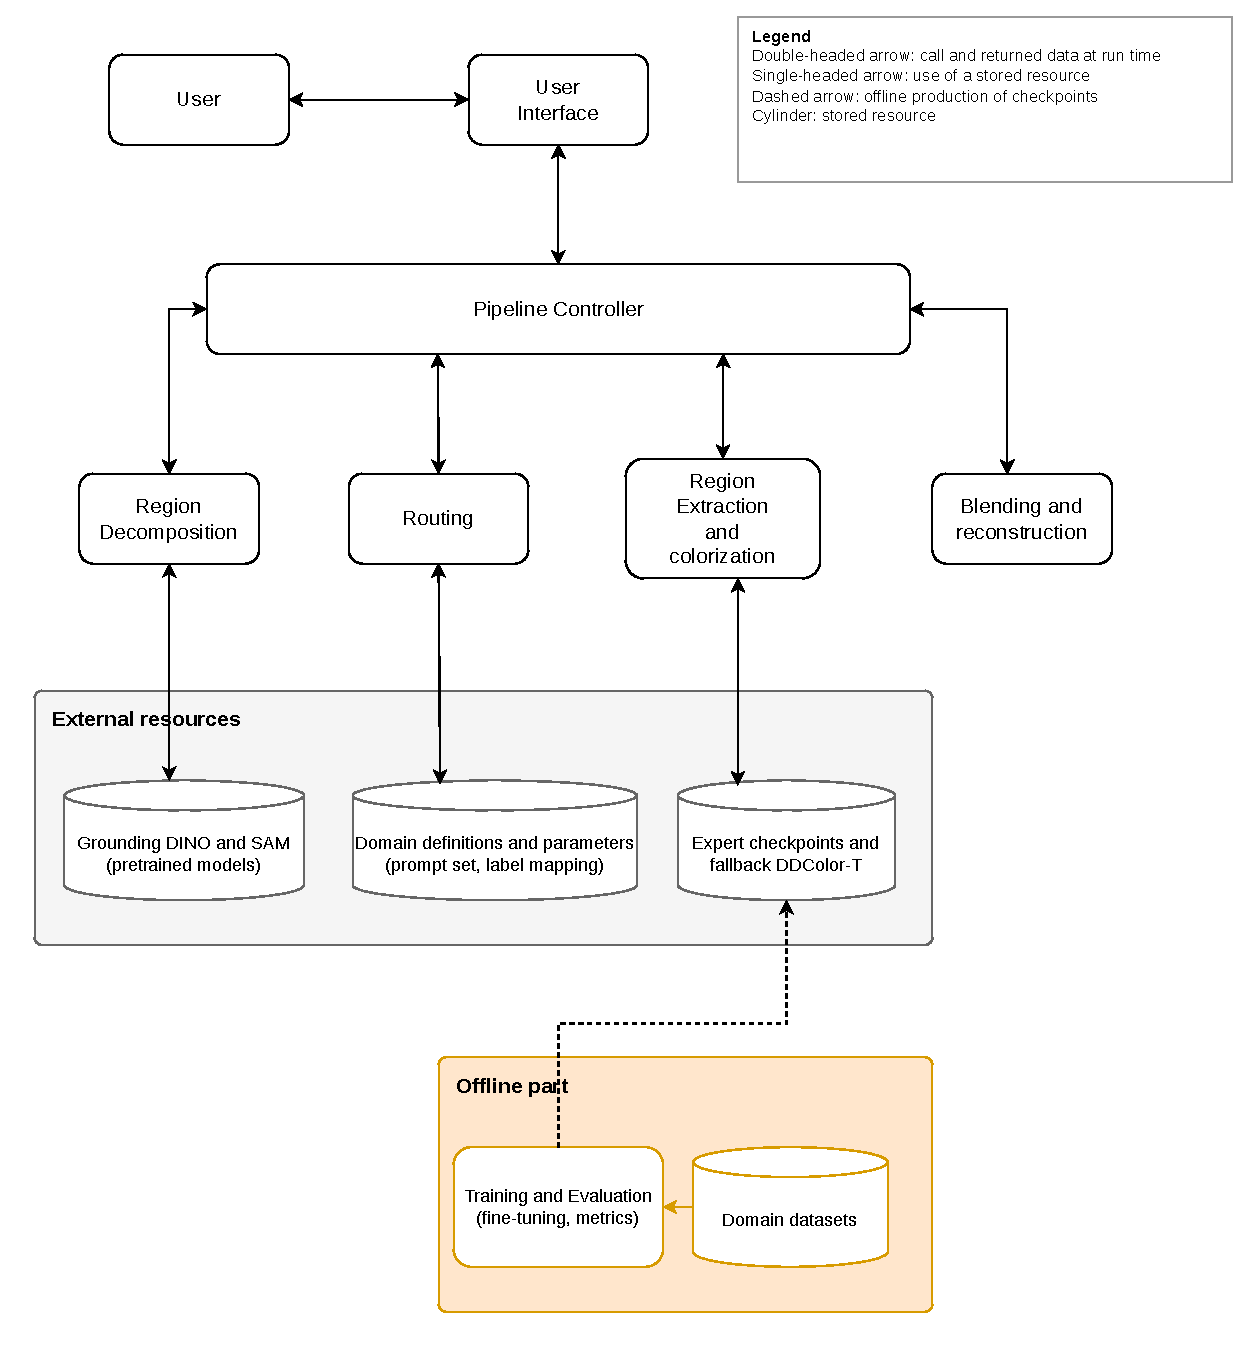
\includegraphics[width=\textwidth,height=0.6\textheight,keepaspectratio]{Figures/architecture-overview.pdf}
    \caption{Top-level architecture of the system.}
    \label{fig:arch-overview}
\end{figure}

The run-time part consists of the following components.

\begin{itemize}
    \item User Interface: receives the uploaded image and displays the result. It contains no colorization logic.
    \item Pipeline Controller: the single entry point of the pipeline. It keeps the original image, calls the subsystems in order, passes the output of each to the next, and returns the final image to the interface. The subsystems do not call each other.
    \item Region Decomposition: finds the regions of the image that belong to the supported domains.
    \item Routing: assigns each region to a domain, makes the regions disjoint, and creates the fallback region for uncovered pixels.
    \item Region Extraction and Expert Colorization: prepares each region as expert input, runs the assigned expert, and places the prediction back into the image.
    \item Blending and Reconstruction: merges the predictions of all regions and combines them with the original luminance.
\end{itemize}

The offline part consists of the Training and Evaluation subsystem, which fine-tunes the experts and measures the results of the system.

The system depends on three pretrained models that it does not modify: Grounding DINO and the Segment Anything Model, used by Region Decomposition, and the DDColor-T checkpoint, which is the starting point of the experts and the fallback expert. The domain datasets are used only by the offline part. Besides these, the subsystems read the domain definitions (the prompt set and the label-to-domain mapping) and the numerical parameters of the method. The subsystems are connected through the data they exchange, which is summarized in Table~\ref{tab:interfaces}.

\begin{table}[htbp]
    \centering
    \caption{Inputs and outputs of the run-time subsystems.}
    \label{tab:interfaces}
    \begin{tabular}{p{4.2cm}p{4.2cm}p{4.2cm}}
        \hline
        \textbf{Subsystem} & \textbf{Input} & \textbf{Output} \\
        \hline
        Region Decomposition & Grayscale image & Regions (mask, label, score, bounding box) \\
        Routing & Regions & Disjoint regions with assigned domains, and the fallback region \\
        Region Extraction and Expert Colorization & Routed regions, luminance & Chrominance map for each region \\
        Blending and Reconstruction & Chrominance maps, masks, original luminance & Color image \\
        \hline
    \end{tabular}
\end{table}

\subsection{Subsystem Architecture}

\subsubsection{Region Decomposition}

The subsystem turns a grayscale image into a list of regions. Figure~\ref{fig:sub-decomp} shows its components.

\begin{figure}[htbp]
    \centering
    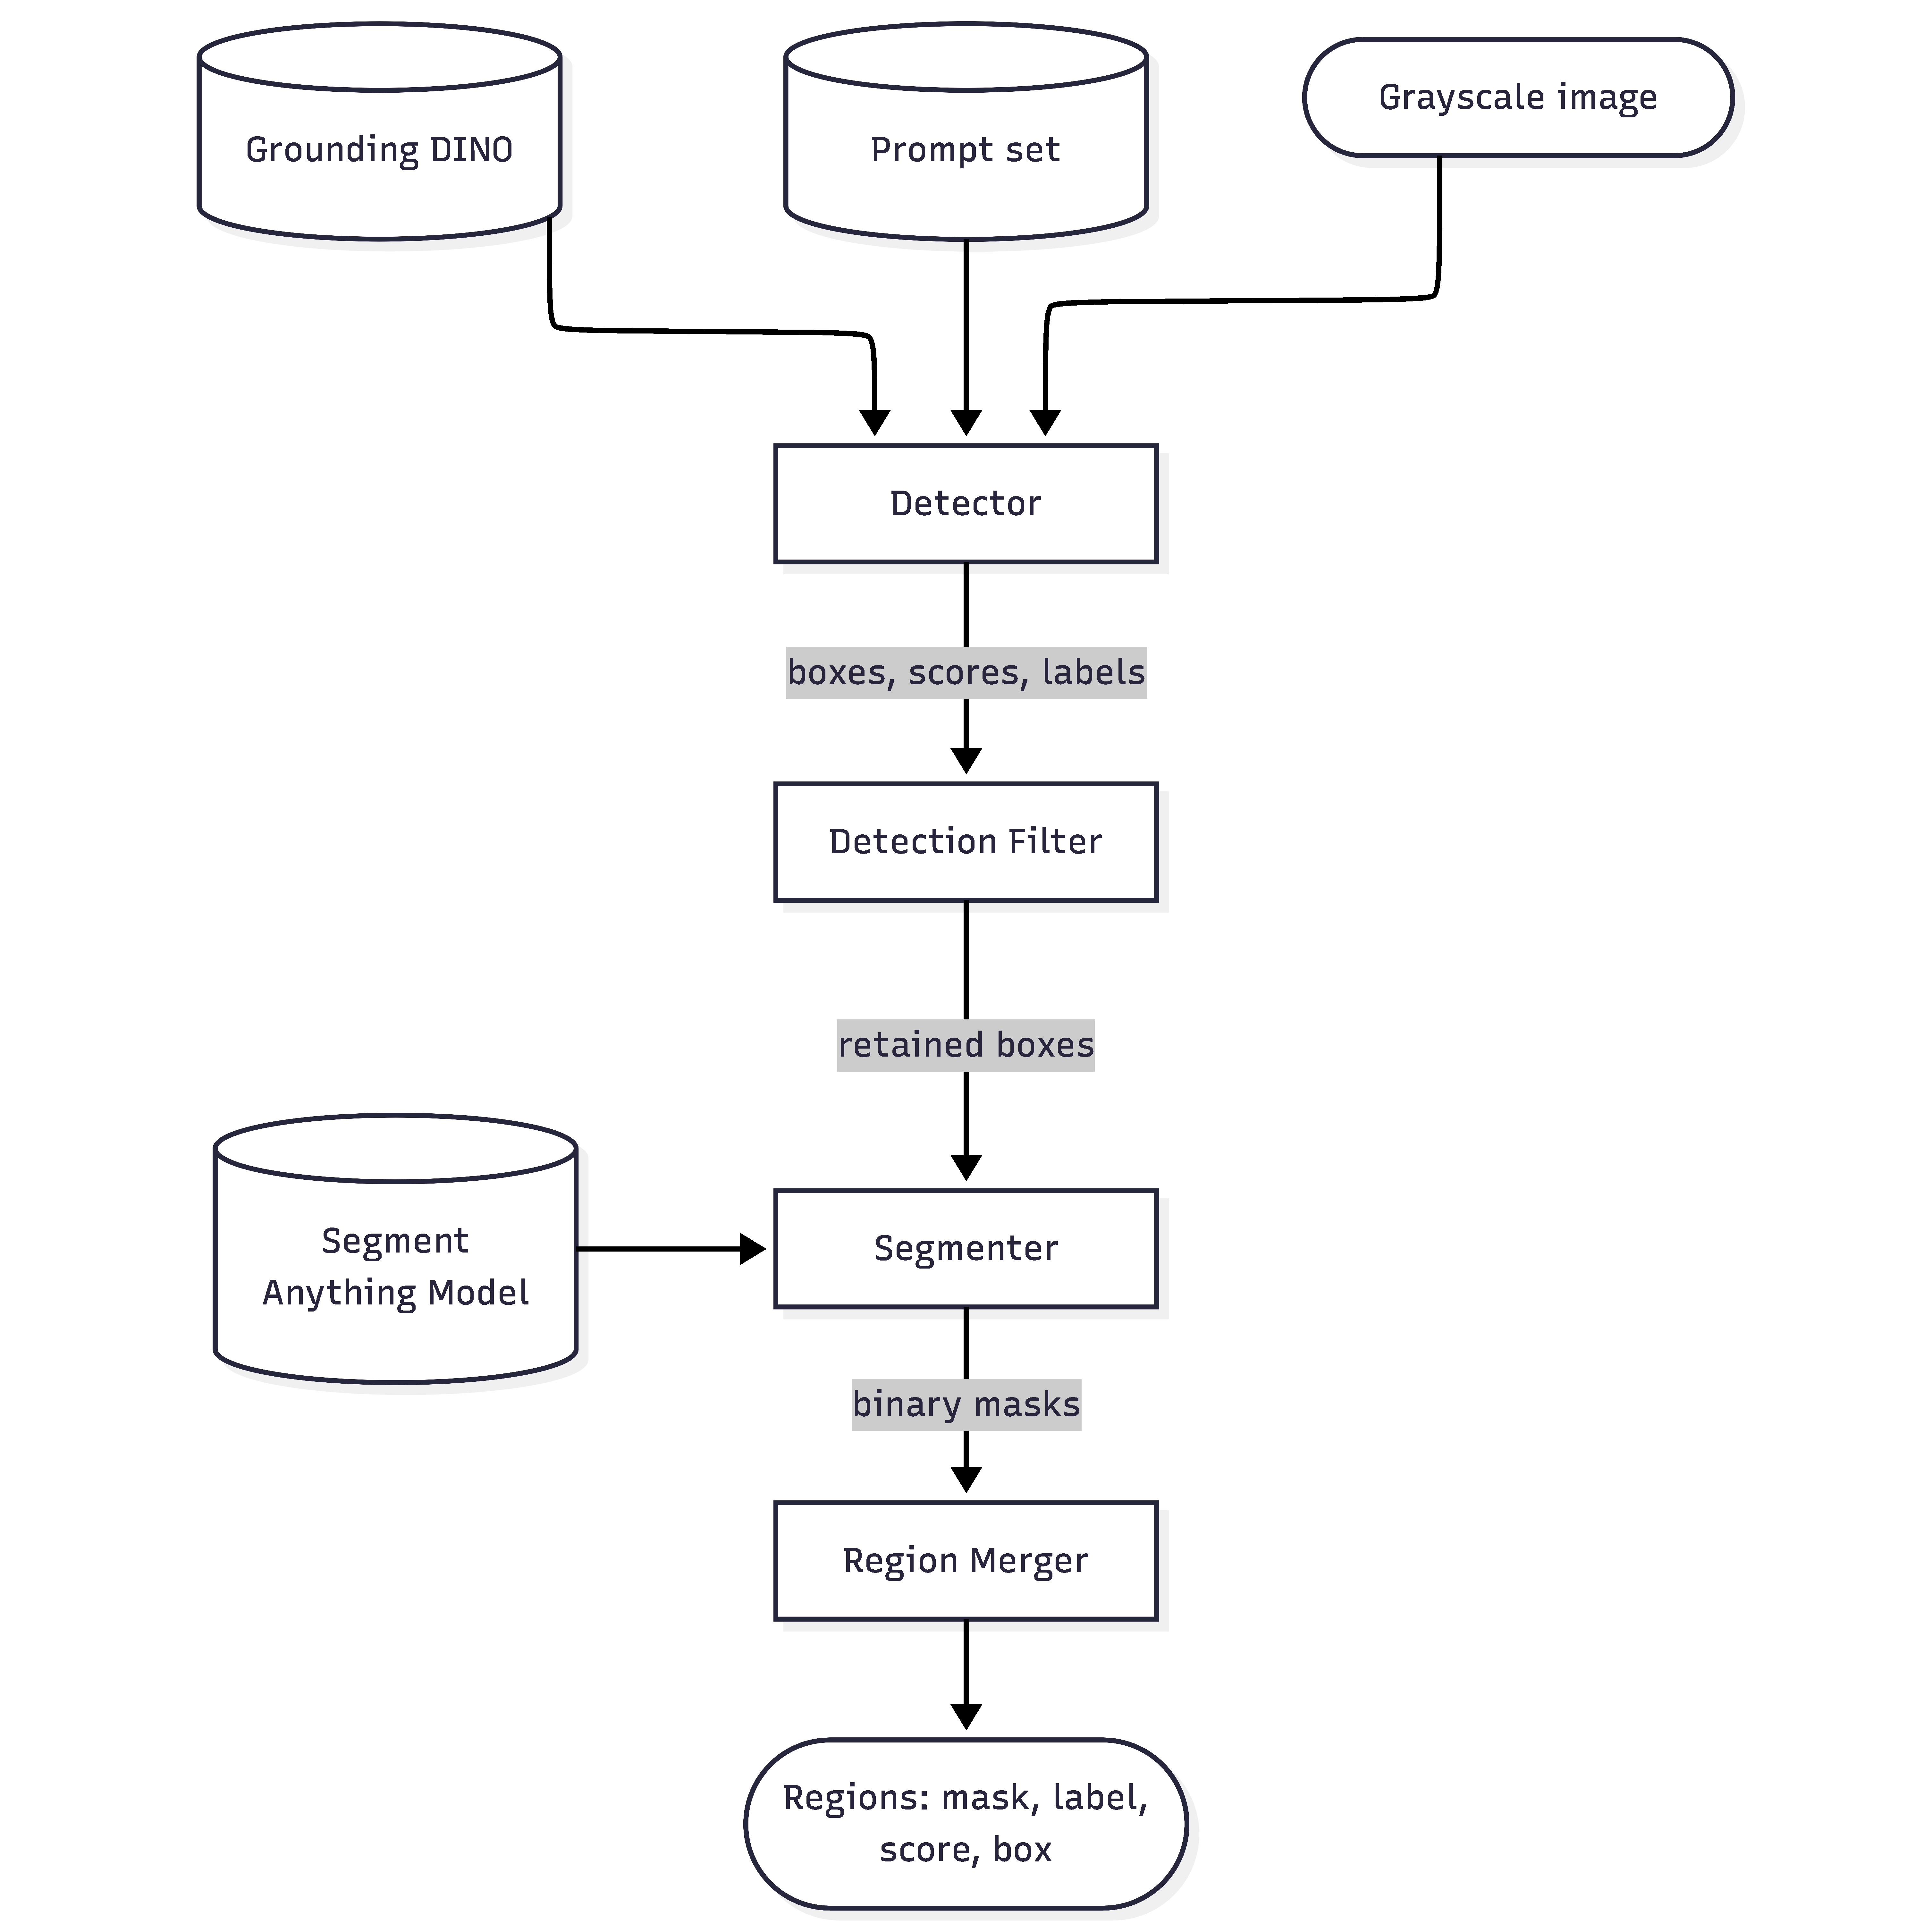
\includegraphics[width=\textwidth,height=0.4\textheight,keepaspectratio]{Figures/subsystem-decomposition.pdf}
    \caption{Components of the Region Decomposition subsystem.}
    \label{fig:sub-decomp}
\end{figure}

\begin{itemize}
    \item Detector: runs Grounding DINO on the image with the prompt set and returns boxes, scores, and labels.
    \item Detection Filter: removes detections below the minimum score and applies per-class non-maximum suppression.
    \item Segmenter: runs the Segment Anything Model with each retained box as a prompt and returns one binary mask per box.
    \item Region Merger: merges the masks of the same label that fragment one object, using the containment rule.
\end{itemize}

The procedure that these components carry out is described in Section~\ref{sec:decomposition}. The subsystem also limits the image size before detection and returns the scale factor, so that the later stages can restore the original resolution.

\subsubsection{Routing}

The subsystem prepares the regions for the experts. Its components are the Label Mapper, which assigns each region the domain of its label and discards regions with an unknown label, the Overlap Resolver, which gives each contested pixel to the smallest region that contains it, and the Fallback Handler, which builds the fallback region from the pixels that no region owns. The rules are given in Section~\ref{sec:routing}.

\subsubsection{Region Extraction and Expert Colorization}

This subsystem produces the chrominance of each region. Figure~\ref{fig:sub-expert} shows its components.

\begin{itemize}
    \item Region Extractor: crops each region with its boundary context, resizes the crop to the expert input size, and places the expert output back at the crop position (Section~\ref{sec:extraction}).
    \item Expert Registry: records which expert belongs to which domain and where its checkpoint is stored.
    \item Expert Manager: loads the checkpoint of an expert when a region is routed to it for the first time, and releases experts that are no longer needed.
    \item Experts: one DDColor-T instance for each domain, with independent weights.
    \item Fallback Expert: the pretrained DDColor-T checkpoint as released, which colorizes the fallback region from the whole image.
\end{itemize}

\begin{figure}[htbp]
    \centering
    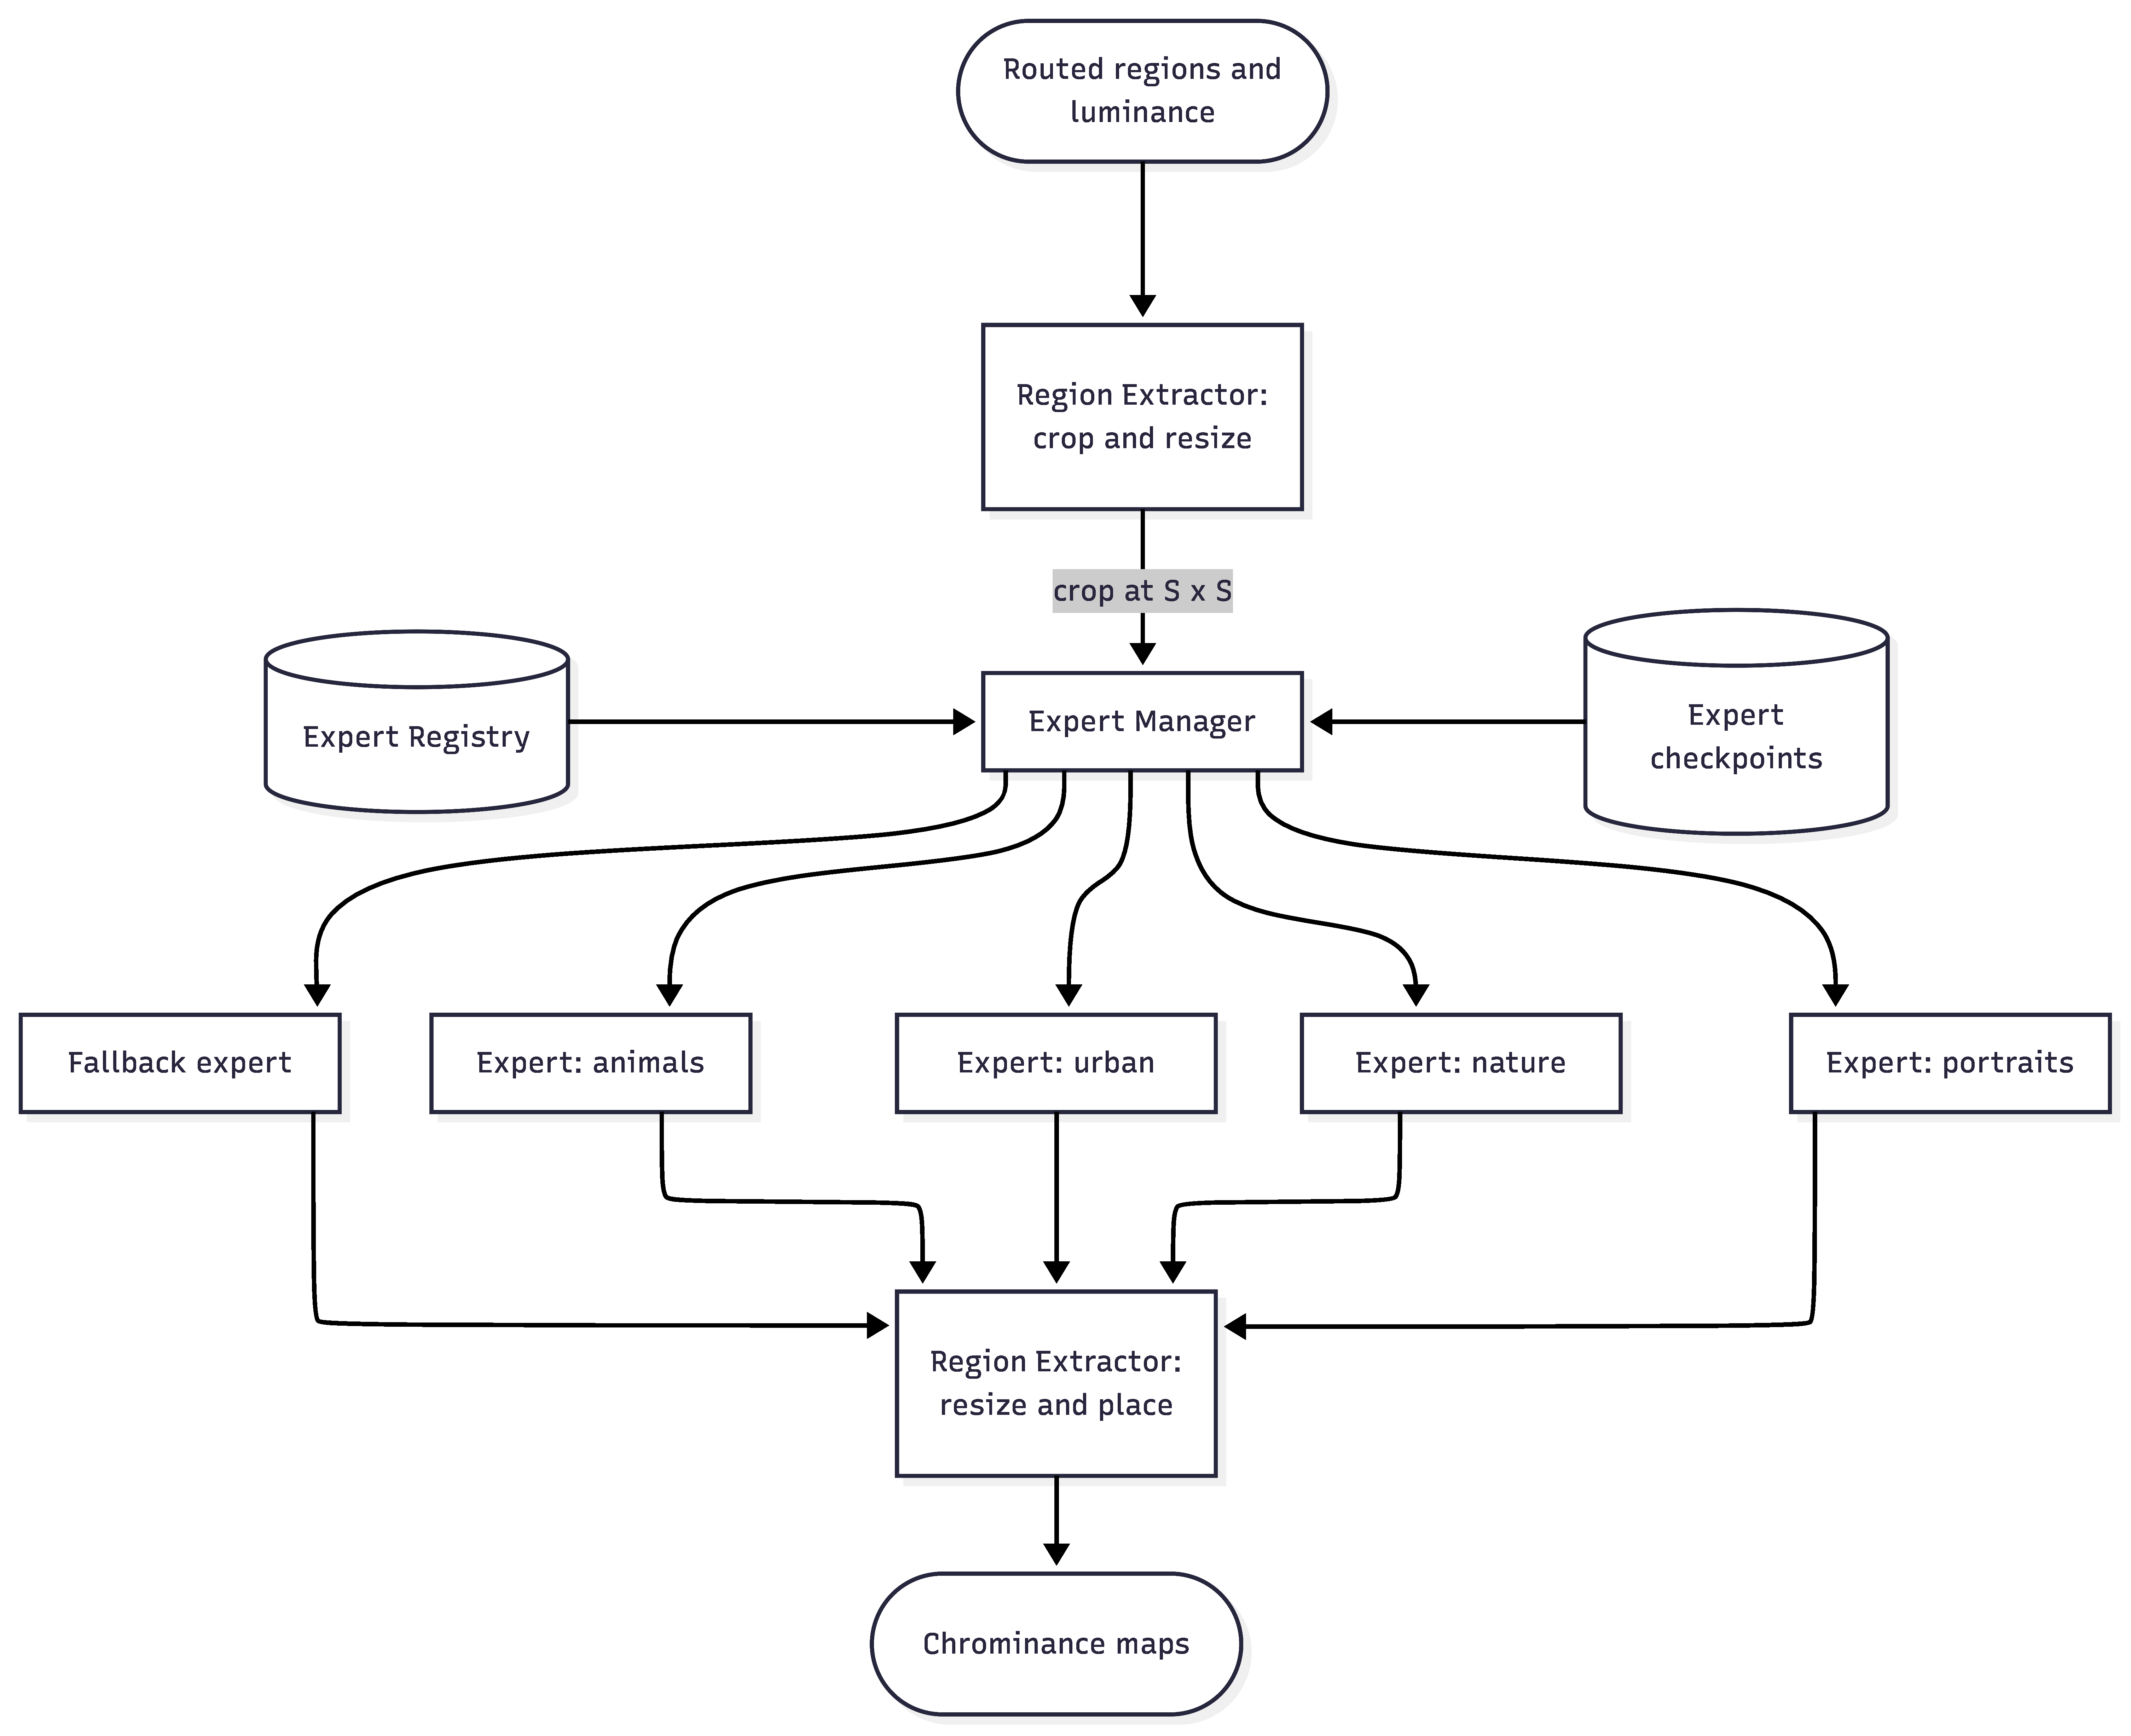
\includegraphics[width=\textwidth,height=0.55\textheight,keepaspectratio]{Figures/subsystem-expert.pdf}
    \caption{Components of the Region Extraction and Expert Colorization subsystem.}
    \label{fig:sub-expert}
\end{figure}

\subsubsection{Blending and Reconstruction}

The subsystem forms the final image from the per-region predictions (Figure~\ref{fig:sub-blend}). The Soft Mask Builder smooths the region masks, the Chrominance Combiner computes the normalized weighted average of the predictions, and the Luminance Recombiner resizes the combined chrominance to the original size, joins it with the original luminance, and converts the result to RGB (Section~\ref{sec:blending}).

\begin{figure}[H]
    \centering
    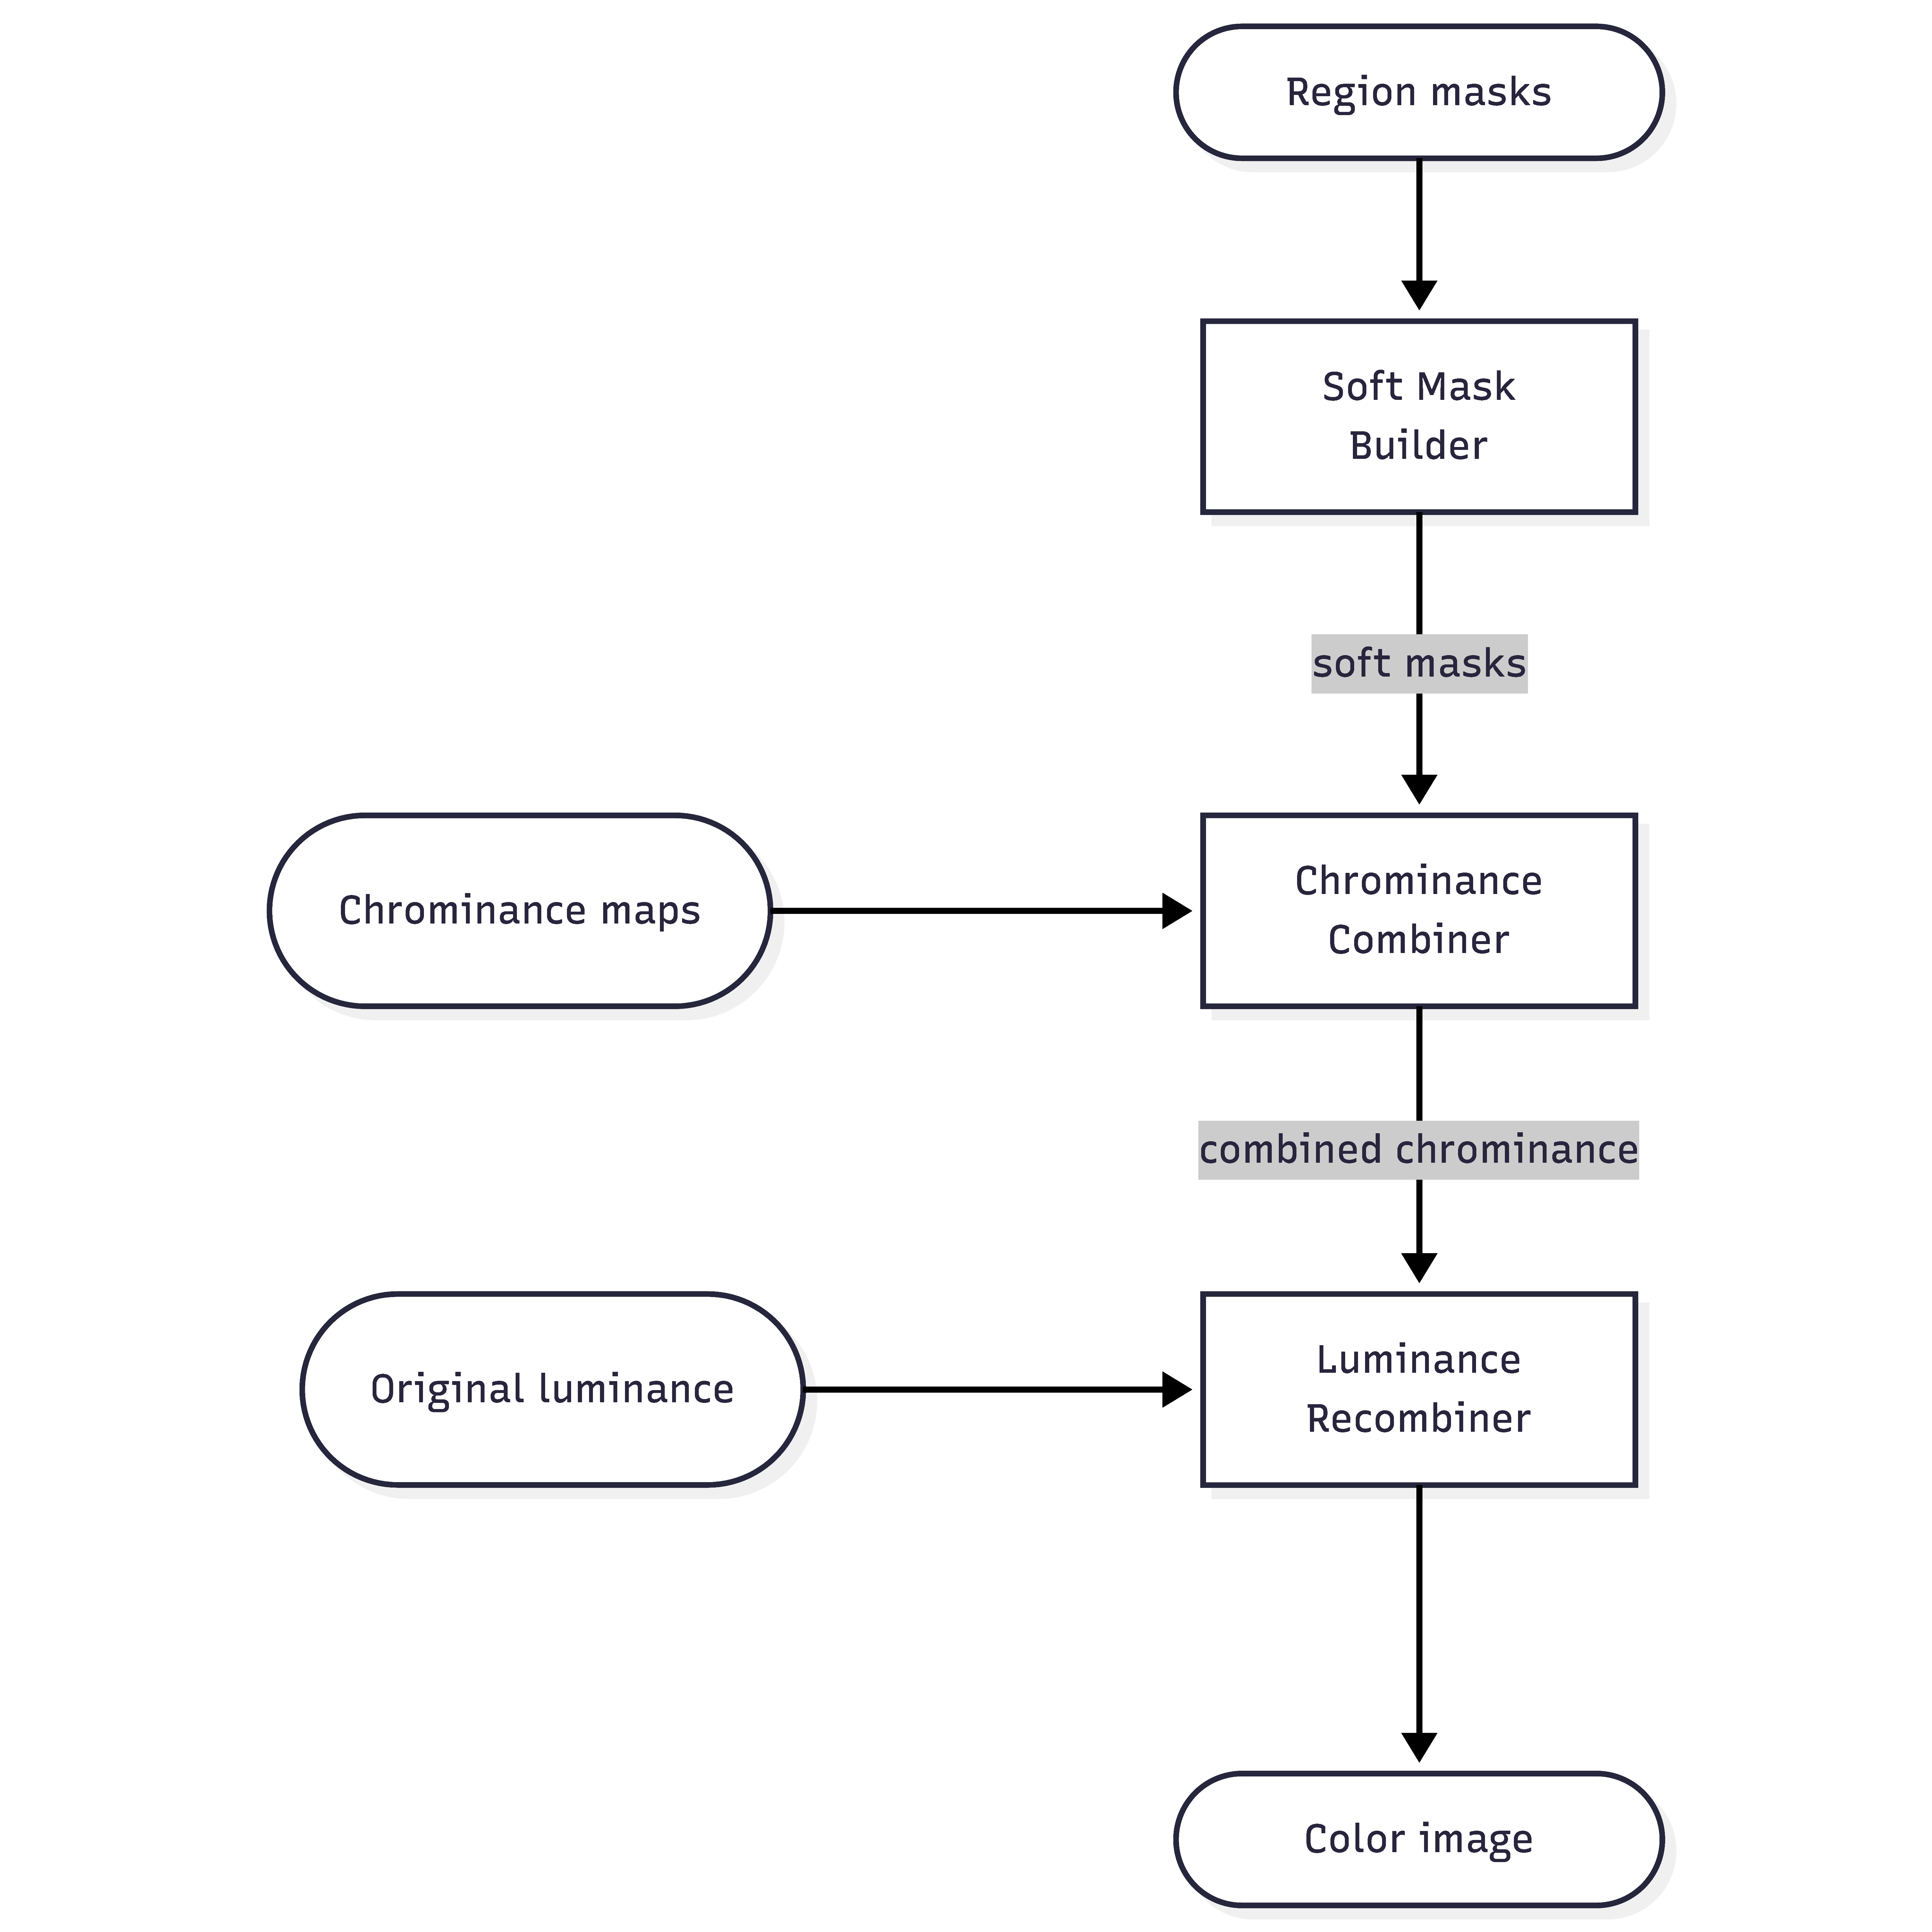
\includegraphics[width=\textwidth,height=0.55\textheight,keepaspectratio]{Figures/subsystem-blending.pdf}
    \caption{Components of the Blending and Reconstruction subsystem.}
    \label{fig:sub-blend}
\end{figure}

\subsubsection{User Interface}

The interface is a basic web page with an upload control, a control that starts the colorization, and a display of the result. It sends the image to the Pipeline Controller and shows the returned image. Because it only exchanges images with the controller, the pipeline can be run without it, which the evaluation scripts do.

\subsubsection{Training and Evaluation}

This offline subsystem is carried out by the developers and takes no part in the processing of an uploaded image. The developers build the training, validation, and test splits of each domain and convert the images to the Lab color space. They then fine-tune a copy of the pretrained DDColor-T checkpoint for each domain (Section~\ref{sec:training}) and compute the metrics of Section~\ref{sec:evaluation} for the system, the baselines, and the ablations. The expert checkpoints that result from the fine-tuning are the only output of this subsystem that the run-time part reads.

\subsection{Interaction Scenarios}

Figure~\ref{fig:seq-colorize} shows the interaction when a user colorizes an image. The user's messages go to the interface, which passes the image to the controller. The controller calls the subsystems in order, and the expert is called once for each region. If the uploaded file is not a valid image, the interface returns an error message and the pipeline is not started.

\begin{figure}[H]
    \centering
    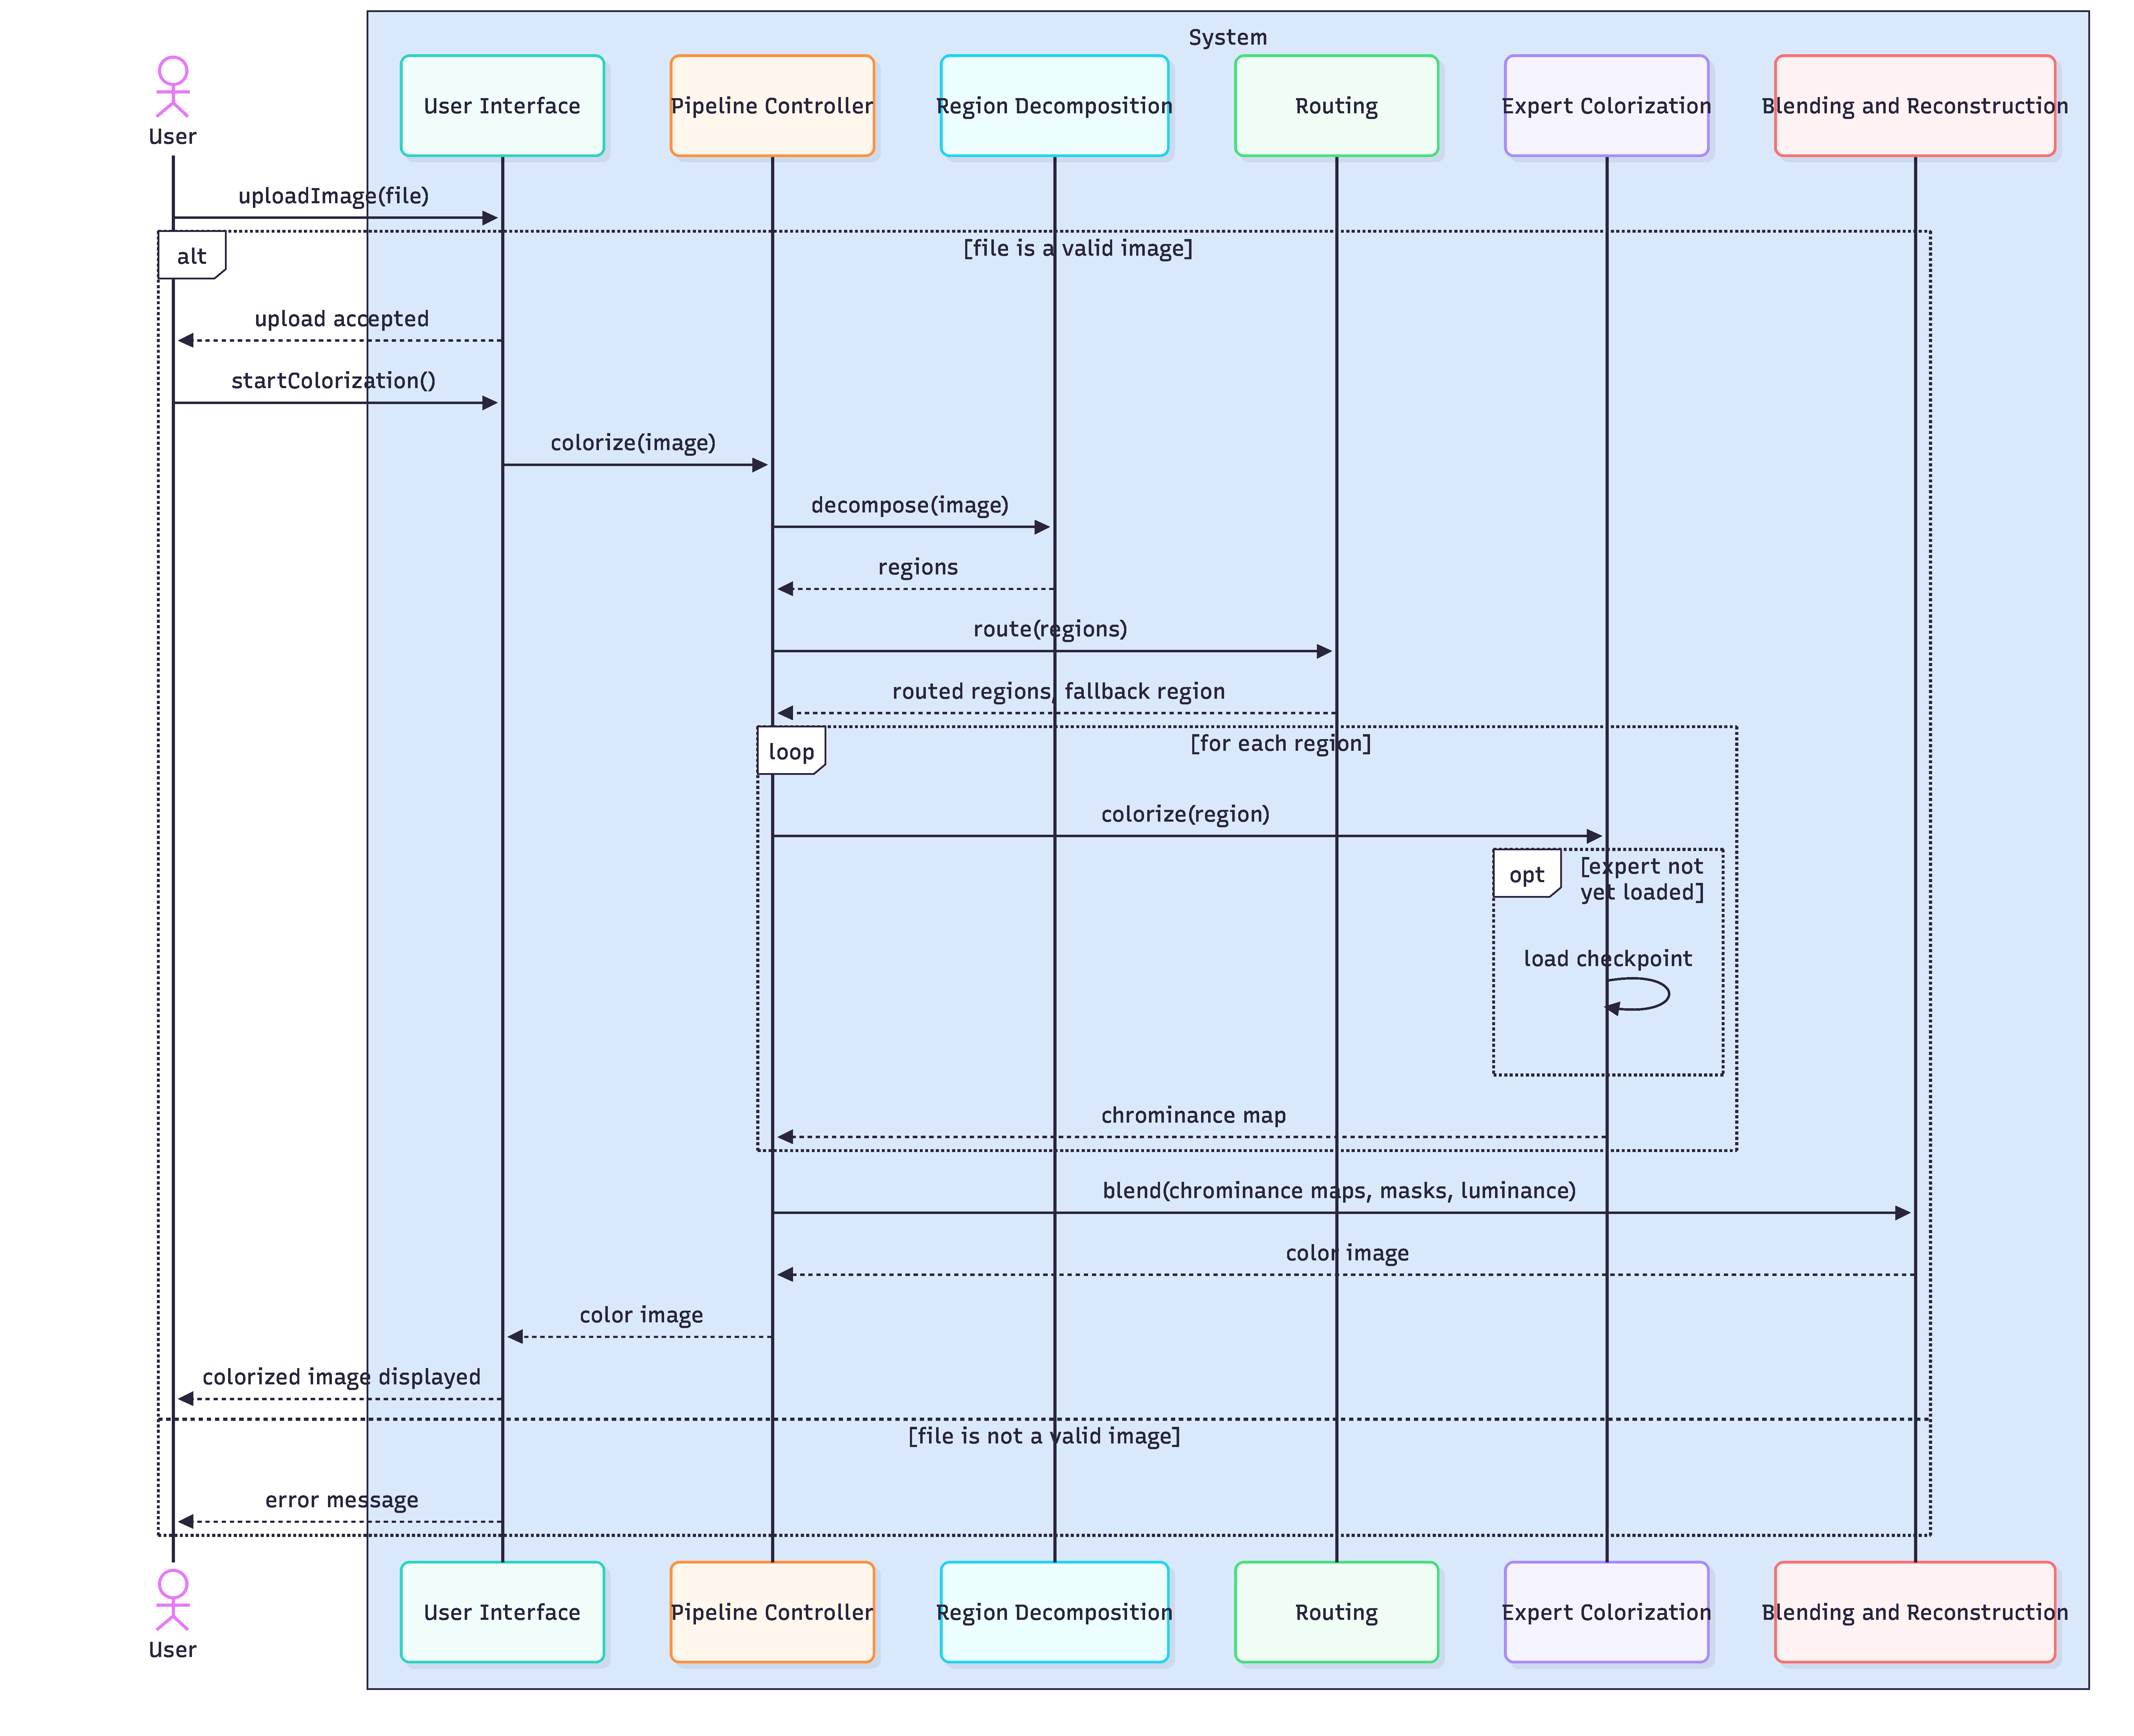
\includegraphics[width=\textwidth,height=0.75\textheight,keepaspectratio]{Figures/sequence-system.pdf}
    \caption{System sequence diagram of colorizing an image.}
    \label{fig:seq-colorize}
\end{figure}

Figure~\ref{fig:seq-addexpert} shows the steps of Section~\ref{sec:extensibility} from the point of view of a developer. The developer defines the prompts and the label mapping of the new domain, builds the dataset splits, and fine-tunes the expert from the pretrained checkpoint. The developer then registers the checkpoint in the Expert Registry and colorizes test images through the Pipeline Controller to run the extensibility test. The comparison of checksums and the evaluation of the results are carried out by the developer. The existing experts take no part in any of the steps.

\begin{figure}[H]
    \centering
    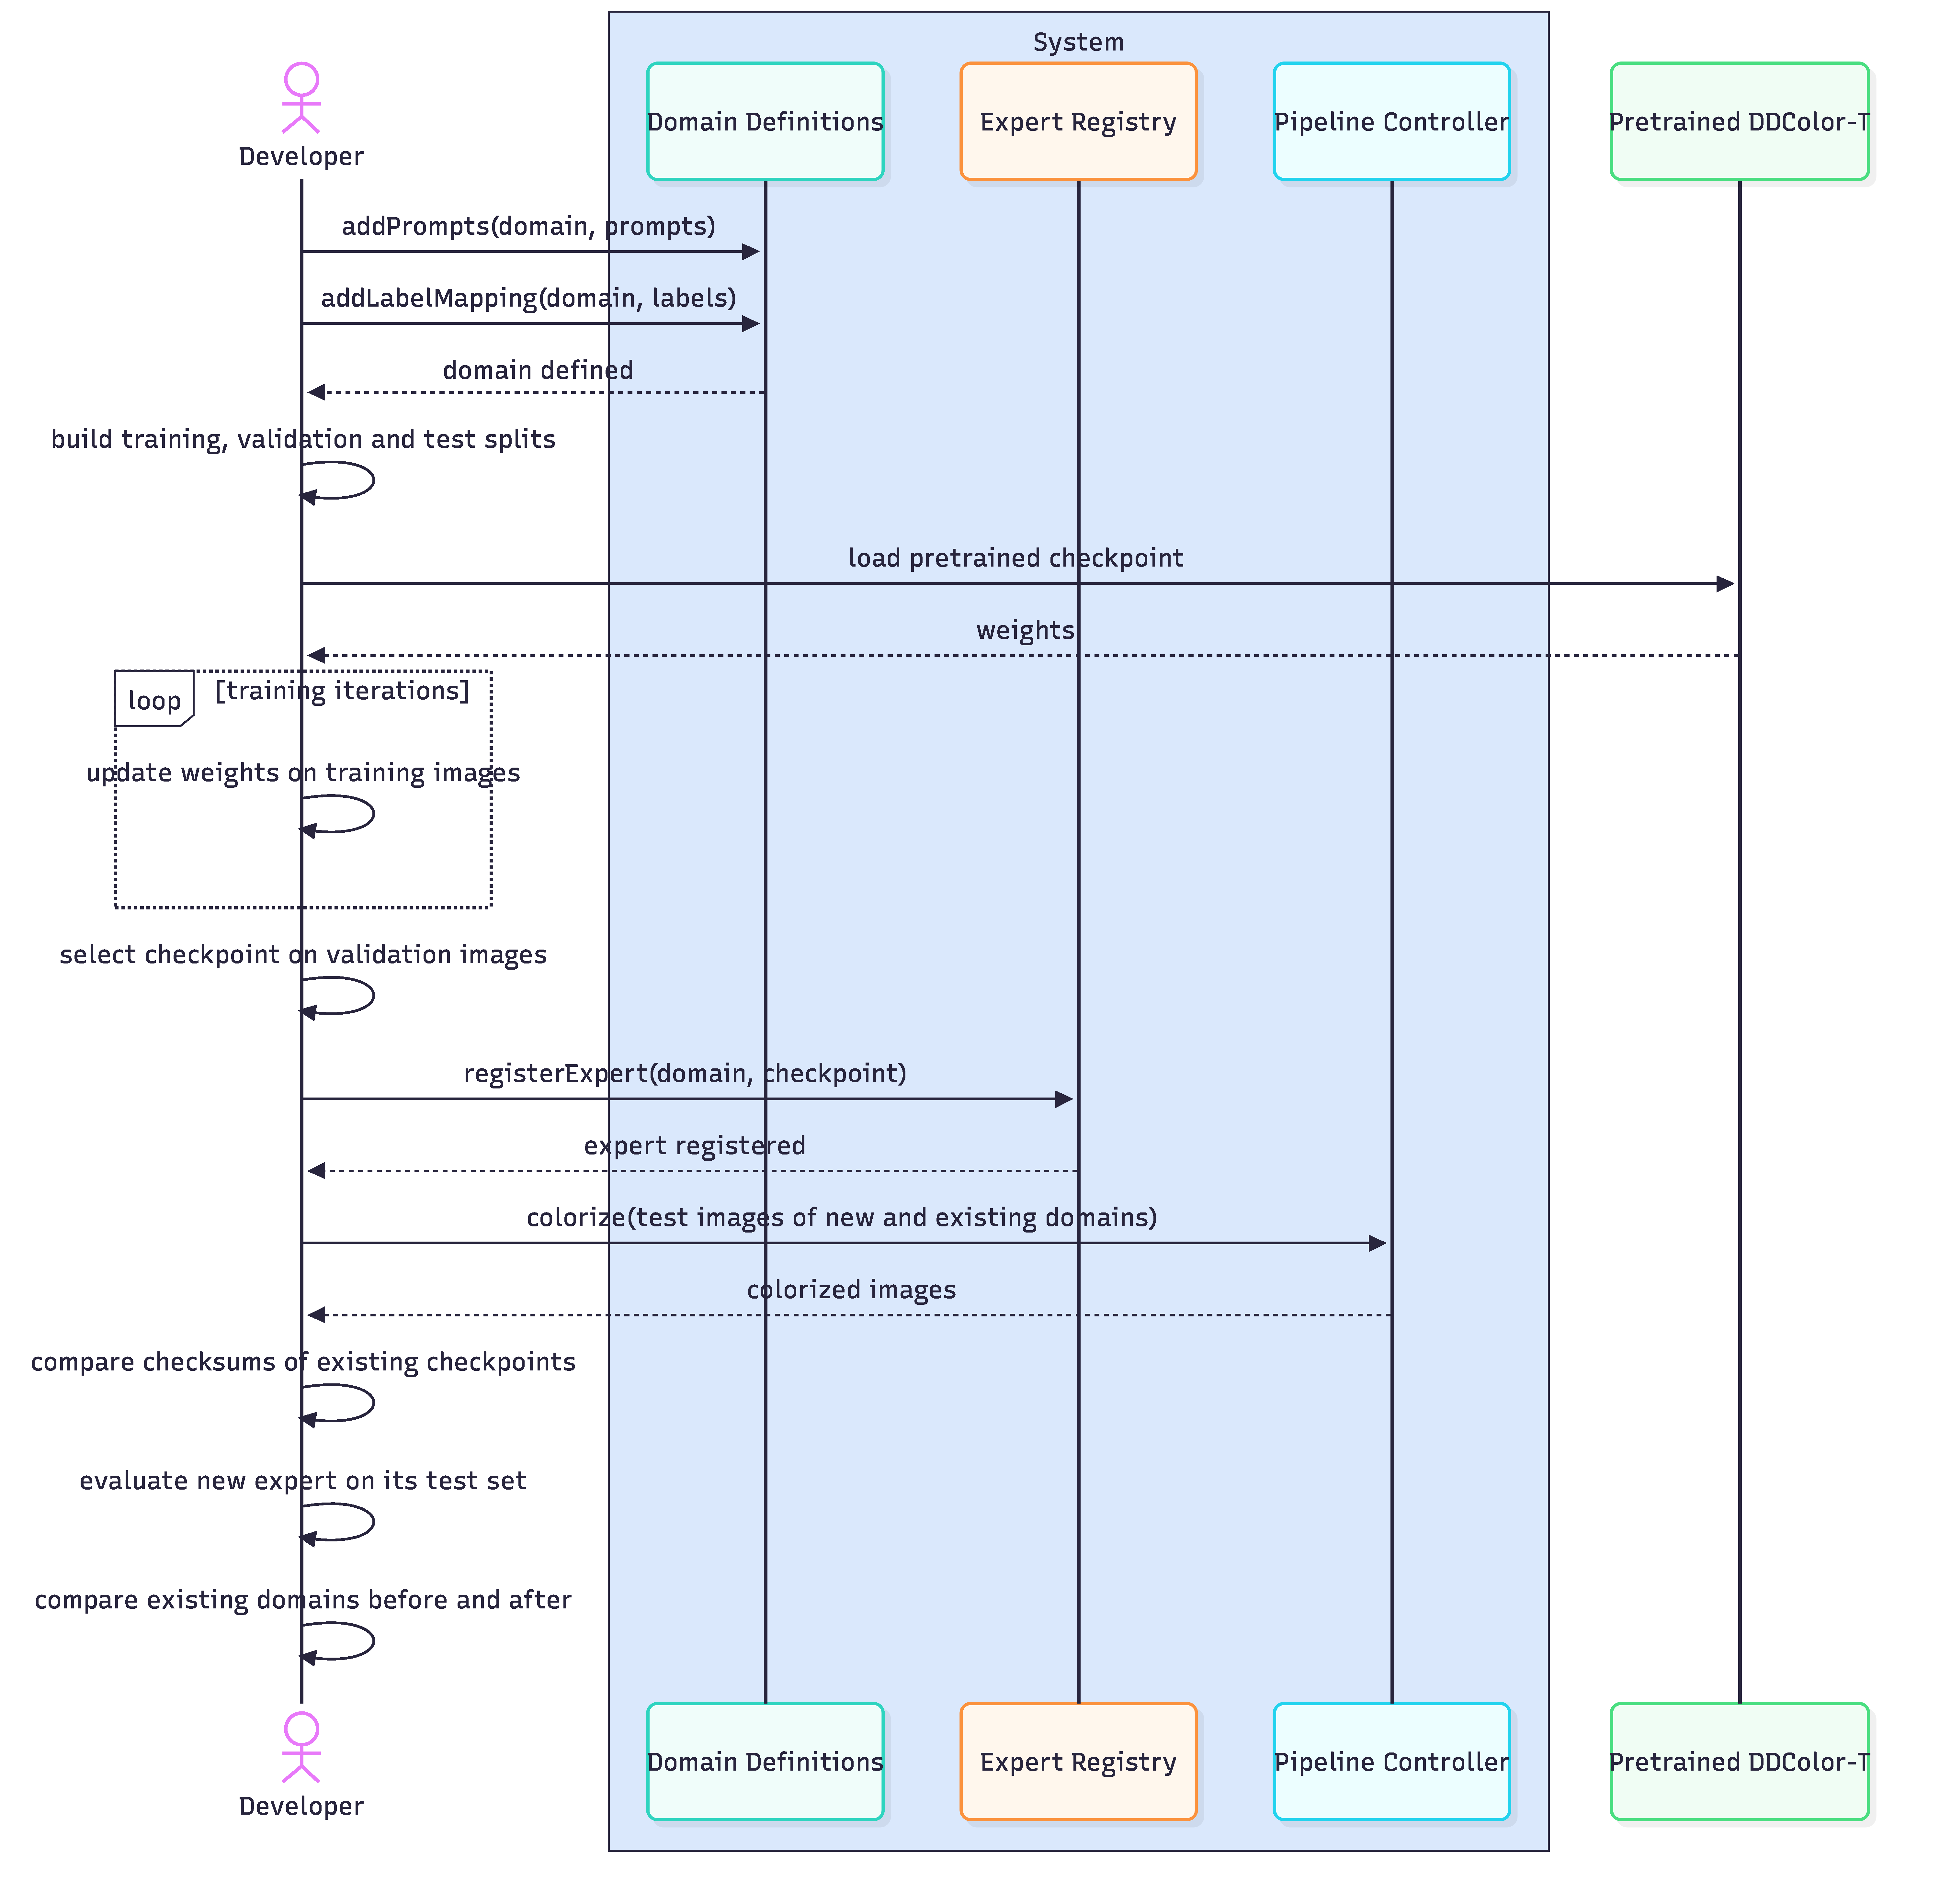
\includegraphics[width=\textwidth,height=0.75\textheight,keepaspectratio]{Figures/sequence-add-expert.pdf}
    \caption{Sequence diagram of adding a new expert.}
    \label{fig:seq-addexpert}
\end{figure}

\subsection{Rationale for the Decomposition}

The system is divided along the stages of the method, and each subsystem has one responsibility and a defined input and output. This makes each stage testable on its own, and it means that the segmentation models, the routing rules, or the expert architecture can change without changes to the other subsystems. Three other decompositions were considered.

\begin{itemize}
    \item A single script containing the whole method. This is the quickest to write, but a change to one stage requires changes throughout, and the stages cannot be tested separately. It was rejected.
    \item An end-to-end Mixture-of-Experts network with a learned gating router. This is the usual form of Mixture-of-Experts. It would require training the router together with the experts, and adding an expert would require retraining the router, which conflicts with the extensibility objective. It was rejected.
    \item Closed-set semantic segmentation in place of Grounding DINO and the Segment Anything Model. It would replace two models by one, but the set of regions would be fixed by its label set, so a new domain would require retraining the segmentation model. It was rejected.
\end{itemize}

\section{Architectural Strategies}
\label{sec:strategies}

This section describes the main decisions that shaped the architecture, the reasons for them, and the alternatives that were considered. The decisions follow the goals of Section~\ref{sec:considerations}.

\subsection{Staged Pipeline with a Central Controller}

The system is a sequence of stages, and the Pipeline Controller is the only component that calls them (Section~\ref{sec:architecture}). Each stage receives its input from the controller and returns its output to it, and no stage calls another. The controller also keeps the data that later stages need but earlier stages do not produce, namely the original image, the original luminance, and the scale factor of the size limit. The alternative is a chain in which each stage calls the next. It would tie every stage to its successor, so replacing or testing one stage would require the others, and the original image would have to be passed through stages that do not use it. A message-based design with queues between the stages was not considered necessary for a prototype that processes one image at a time.

\subsection{Separation of the User Interface from the Pipeline}

The user interface only sends an image to the controller and displays the image it returns. It contains no colorization logic. The reason is that the same pipeline must be run by the evaluation scripts without an interface, and that the interface can be changed without affecting the pipeline. The alternative of placing processing steps in the interface code would make the pipeline impossible to test without the interface.

\subsection{Reuse of Pretrained Models}

Region decomposition and the starting point of every expert rely on pretrained models (Section~\ref{sec:considerations}). The reason is the compute budget, which does not allow training a detector, a segmentation model, and four colorization networks from scratch. Each pretrained model is used through a thin wrapper that defines the input and output of the stage and hides the library-specific calls. The wrapper limits the effect of a change of model or library version to one component. The cost of the strategy is a dependence on the availability and licensing of third-party models, which is addressed by recording the versions that are used.

\subsection{Common Architecture with Independent Weights}

All experts use the same network architecture, and each expert has its own weights, trained separately (Section~\ref{sec:experts}). Three alternatives were considered. A frozen shared backbone with small per-domain adapters would save storage, but the experts would then share parameters, and a change to the shared part would affect all of them. A single network conditioned on the domain would also share all parameters, and adding a domain would require retraining it. Different architectures for different experts would add code for each one and would mix the effect of the architecture with the effect of the training data in the evaluation. The chosen design keeps each expert replaceable on its own and keeps the comparison between experts and baselines clean.

\subsection{Registry-Driven Extensibility}

The domains known to the system are data and not code. The prompt set, the label-to-domain mapping, and the expert registry are read when the system starts, and the stages use them without reference to specific domains. Adding a domain therefore means adding entries and a checkpoint, and no stage changes (Section~\ref{sec:extensibility}). The alternatives are to write the domains into the code, for example as a chain of conditions, which requires code changes for each new domain, or to use a learned router, which would have to be retrained whenever a domain is added.

\subsection{Chrominance-Only Prediction with Luminance Preservation}

The networks predict only the chrominance channels, and the output uses the luminance of the original image at full resolution (Section~\ref{sec:blending}). The alternative of predicting a full RGB image would make the network responsible for structure and brightness that the input already contains, and enlarging its output would blur that detail. With the chosen strategy, the fine detail of the photograph does not pass through the networks, which operate at a reduced size, and only the chrominance is enlarged.

\subsection{Memory Management}

The segmentation models are used for every image and stay loaded. An expert is loaded when a region is first routed to it, and it is released when the image has been processed. The size of the processed image is limited (Section~\ref{sec:decomposition}) so that the memory needed for the activations of the models has an upper bound. The weights of the four experts occupy less than 1 GB in 32-bit precision, so memory is not limiting at the present number of experts. Loading on demand is chosen so that memory use does not grow with the number of experts, which matters because the system is meant to be extended. The alternative of keeping all experts loaded is simpler and faster at run time, but the memory it requires increases with every added expert. To limit the time lost to loading, the regions of an image are processed in order of their expert, so that each expert is loaded at most once per image.

\subsection{Error Detection and Recovery}

The system either returns a complete colorized image or reports an error. It never returns a partly colorized image. The following situations are handled.

\begin{itemize}
    \item Invalid input. A file that is not a valid image is rejected before the pipeline starts, and the user receives an error message.
    \item No region detected, or a label that cannot be routed. The pixels concerned are uncovered, and the fallback expert colorizes them (Section~\ref{sec:fallback}). If no region is found, the whole image is colorized by the fallback expert.
    \item Empty region after overlap resolution. A region whose mask has no remaining pixels is dropped (Section~\ref{sec:overlap}).
    \item Missing or unreadable expert checkpoint. The regions of that expert are given to the fallback expert, and a warning is recorded.
    \item Insufficient memory. The request fails with an error message and no partial result is returned.
\end{itemize}

\subsection{Control Flow and Concurrency}

The stages run one after the other, since each needs the output of the previous one. Inside the expert stage, regions are processed one at a time. Regions routed to the same expert all have the same input size, so they could be processed together in a single batch, which is a possible optimization that the prototype does not use. Requests are handled one at a time, because the system runs on a single GPU and serves one user at a time. Handling several requests at once would add scheduling and memory management that a prototype does not need.

\section{Domain Model and Class Diagram}
\label{sec:classdiagram}

Figure~\ref{fig:classdiagram} shows the classes. The upper part contains the interface and the controller. Below them, the classes are arranged in four columns, one for each subsystem of Section~\ref{sec:architecture}: region decomposition, routing, extraction and expert colorization, and blending. The first class of each column is the class that the controller calls, and the classes below it are its components. The data classes that the subsystems exchange are shown at the bottom.

\begin{figure}[htbp]
    \centering
    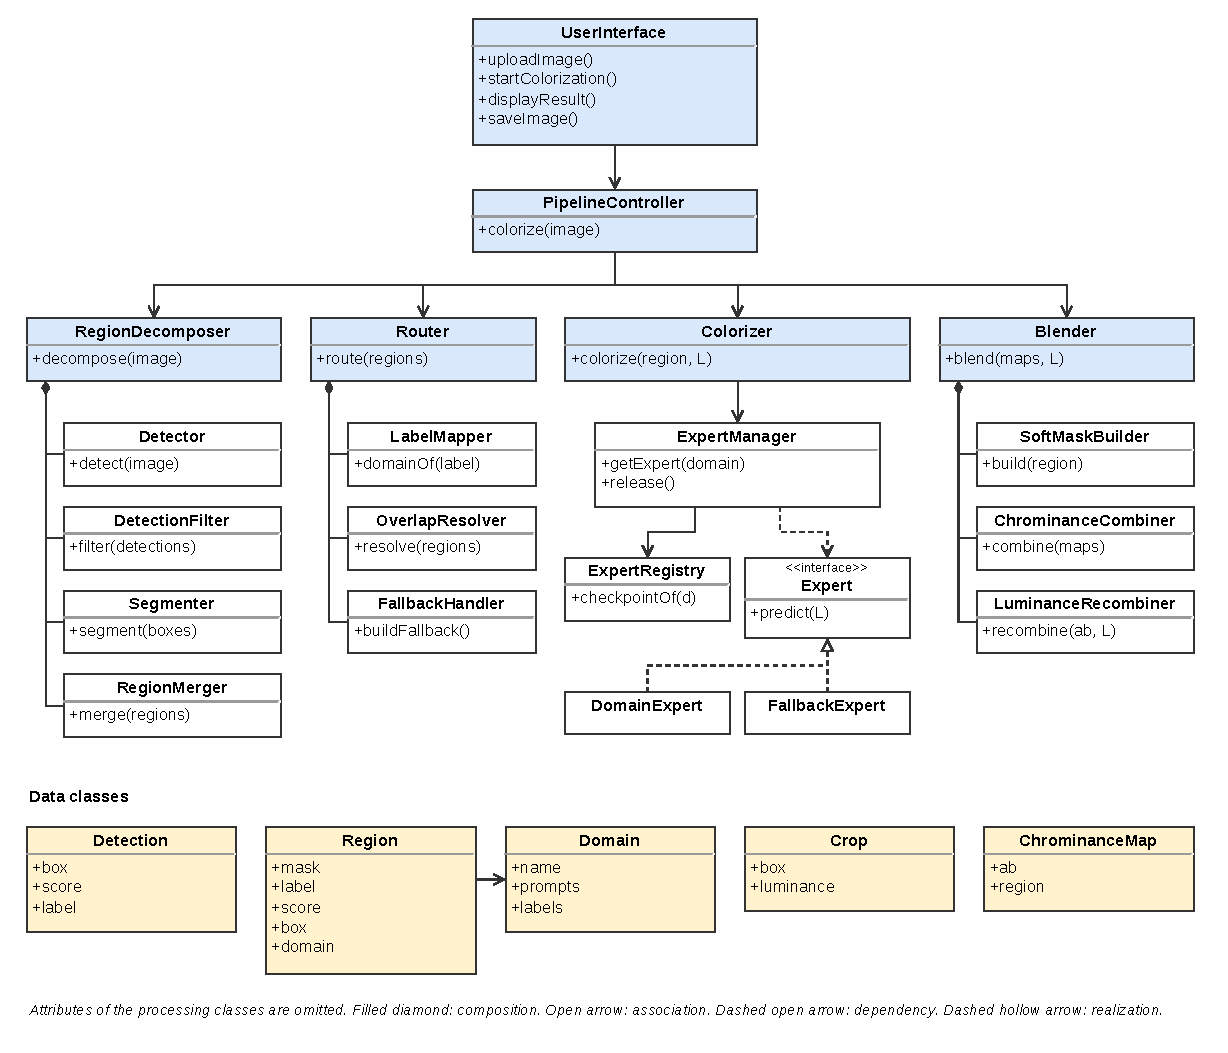
\includegraphics[width=\textwidth]{Figures/class-diagram}
    \caption{Class diagram of the run-time pipeline.}
    \label{fig:classdiagram}
\end{figure}


\section{Policies and Tactics}
\label{sec:policies}

\subsection{Tools and Libraries}

The pipeline is written in Python. The networks run on PyTorch, and the pretrained models are used through the libraries released with them. The web interface is built with Next.js for the frontend and FastAPI for the backend that exposes the pipeline to it. Library and model versions are fixed, because the released code of the pretrained models depends on specific versions.

\subsection{Coding Conventions}

The code follows the PEP~8 style guide. Each class of Figure~\ref{fig:classdiagram} is placed in its own module, and each class and public method has a short docstring that states its input and output. Each stage is called only through the interface of its entry class, so that no module depends on the internals of another.

\subsection{Testing}

Each stage is tested alone with small fixed inputs: for example the filter on a list of detections with known scores, the overlap resolver on two overlapping masks, and the blender on two regions with known chrominance. The complete pipeline is then run on a few test images and the intermediate results are inspected visually. The quality of the system is measured with the evaluation of Section~\ref{sec:evaluation}, and not by these tests.

\subsection{Reproducibility and Maintenance}

Library versions, model checkpoint names, and random seeds are recorded with each experiment (Section~\ref{sec:considerations}). Changes to the prompt set, the label mapping, or the list of experts are made as data changes and do not modify the code of the stages (Section~\ref{sec:strategies}).

\subsection{Traceability}

Table~\ref{tab:traceability} relates each project objective to the components that implement it and to the part of the evaluation that tests it.

\begin{table}[htbp]
    \centering
    \caption{Relation between objectives, components, and evaluation.}
    \label{tab:traceability}
    \begin{tabular}{p{3.4cm}p{5.4cm}p{4.2cm}}
        \hline
        \textbf{Objective} & \textbf{Components} & \textbf{Evaluation} \\
        \hline
        Region decomposition & RegionDecomposer and its components & mIoU (Section~\ref{sec:evaluation}) \\
        Expert colorization quality & RegionExtractor, ExpertManager, experts & FID, LPIPS, PSNR, SSIM, $\Delta E$ \\
        Routing & Router, LabelMapper, OverlapResolver & Routing accuracy \\
        Blending & Blender and its components & Boundary $\Delta E$, FID, LPIPS \\
        Extensibility & ExpertRegistry, Domain & Extensibility test \\
        \hline
    \end{tabular}
\end{table}

\section*{Conclusion}

This chapter presented the design of the colorization system. The system is a pipeline of subsystems that are called in order by a controller: region decomposition, routing, expert colorization, and blending. A basic web interface sits on top of it. The design follows the goals of modularity, extensibility, and preservation of the input, and it works within the limits of a single GPU of moderate memory. The class diagram defines the classes that implement the subsystems, and the policies describe how they are built and tested. The next chapter describes the implementation and reports the results of the evaluation.



\chapter{Implementation and Test Cases}
This chapter describes the implementation of the region-based Mixture-of-Experts colorization pipeline, the evaluation tooling, and the test cases. It covers the five pipeline stages (decomposition, routing, extraction, colorization, blending), the configuration system, the web interface prototype, the E4 ablation runner, the extensibility mechanism, and the evaluation metrics with fixed test sets. The implementation follows the design of Chapter~\ref{ch:design} and produces the experimental results reported in Chapters~8 and~9.

\section{Implementation}
This section describes the implementation of the region-based Mixture-of-Experts colorization pipeline. The five stages are decomposition, routing, extraction, colorization, and blending, built as pure NumPy/PyTorch modules. Decomposition and routing logic uses only NumPy and is fully CPU-testable; model weights load lazily. A configuration system centralizes hyperparameters. A CLI and HTML prototype provide the web interface; full Next.js/FastAPI integration is deferred to FYP-2. The E4 ablation runner implements margin-based prediction sharing and CSV-based resumability. Extensibility is achieved through data-driven configuration, so adding a domain requires only data changes.
\subsection{Platform and Tools}
The decomposition and routing stages are written in Python as part of a single package, \texttt{colorize}, which the three team members share through one GitHub repository. The code is split deliberately into two kinds of modules. Modules that call the pretrained models (loading the detector and the segmenter, running them on an image) are kept in one file. Everything else, namely detection filtering, fragment merging, routing, overlap resolution and the evaluation arithmetic, is plain NumPy. This makes that logic testable on any machine without a GPU, and it also means the models are loaded only when the first image is processed, not when the code is imported.
 
All experiments for these stages were run in Kaggle notebooks with a GPU accelerator and internet access, because the university-assigned GPU machine was not available during most of the development period. Table~\ref{tab:a_tools} lists the tools used.

\begin{table}[!ht]
\centering
\caption{Tools and libraries used for decomposition, routing and their evaluation, with exact versions from the Kaggle run.}
\label{tab:a_tools}
\begin{tabular}{|p{2.6cm}|>{\raggedright\arraybackslash}p{5.4cm}|>{\raggedright\arraybackslash}p{4.4cm}|}
\hline
\textbf{Component} & \textbf{Tool} & \textbf{Role} \\ \hline
Language & Python 3.13.16 (Kaggle runtime, Linux 6.18.55) & Implementation of all stages \\ \hline
Deep learning framework & PyTorch 2.11.0+cu130, torchvision 0.26.0 & Running both pretrained models on the GPU (CUDA 13.0) \\ \hline
Open-vocabulary detector & Grounding DINO, tiny variant (\texttt{IDEA-Research/} \texttt{grounding-dino-tiny}) \cite{liu2024groundingdino} & Turns the text prompts into boxes with scores and labels; loaded through Hugging Face \texttt{transformers} 5.20.2 \\ \hline
Segmentation model & Segment Anything Model, ViT-B (\texttt{segment-anything} 1.0, checkpoint \texttt{sam\_vit\_b.pth}, 375.0\,MB) \cite{kirillov2023sam} & Turns each box into a binary mask \\ \hline
Arrays and images & NumPy 2.1.3, Pillow 13.0.0 & Mask arithmetic, grayscale conversion, Lanczos resizing \\ \hline
Figures & Matplotlib 3.10.0 & Confusion matrices and example grids \\ \hline
Testing & pytest & Automated unit tests \\ \hline
Version control & Git and GitHub & Shared code base \\ \hline
Compute & Kaggle notebooks, GPU accelerator T4 & All E1 and E2 runs \\ \hline
\end{tabular}
\end{table}


\subsection{Implementation of Region Decomposition}
The decomposition stage takes one image and returns the list of regions that the rest of the pipeline works on. It follows the procedure of Section~5.2 and is implemented in six steps, which are applied in this order.
 
\paragraph{Step 1: loading.} The image is read as a single-channel grayscale image. If its longer side is above the maximum side (1024 pixels), it is shrunk with Lanczos resampling so that the longer side equals 1024 and the aspect ratio is kept. All masks produced later live at this working resolution. Both models expect three-channel input, so the grayscale image is copied into three identical channels before it is passed to them. This is important for the experiments: the detector never sees the original colors, which matches the situation in the real system, where only a grayscale photograph is available.
 
\paragraph{Step 2: text prompt.} All prompts of the four domains are joined into one lowercase string, with every entry followed by a period. For the prompt set used here, the string is
\begin{center}
\texttt{person . face . sky . vegetation . tree . building . animal .}
\end{center}
Because one string covers all classes, the detector is run once per image.
 
\paragraph{Step 3: detection.} Grounding DINO returns a box in pixel coordinates, a confidence score and a text label for every detection. A detection is kept only if its box confidence is above the box threshold and its match with a word of the prompt is above the text threshold. The text labels are taken directly from the detector output and later serve as the routing key.
 
\paragraph{Step 4: filtering.} Detections with a score below the minimum score are dropped. Duplicates are then removed by non-maximum suppression within each class: boxes are visited from the highest to the lowest score, and any not-yet-removed box with the same label whose intersection over union with the visited box is greater than the suppression threshold is removed. The intersection over union of two boxes $b_1$ and $b_2$ is
\begin{equation}
\mathrm{IoU}(b_1,b_2)=\frac{|b_1\cap b_2|}{|b_1|+|b_2|-|b_1\cap b_2|}.
\end{equation}
Boxes with different labels never remove each other, so a person in front of a building keeps both boxes.
 
\paragraph{Step 5: segmentation.} The segmentation model encodes the image once. Every retained box is then given to it as a box prompt, and the model returns one binary mask per box. Only the first (single) mask output is used.
 
\paragraph{Step 6: merging fragments.} Several boxes can cover parts of the same object, and their masks then appear as fragments. Masks are visited from the largest to the smallest area. For each mask that has not been merged yet, every other unmerged mask with the same label is absorbed into the group when its containment is above the merge threshold, where
\begin{equation}
\mathrm{containment}(M_g, M_c)=\frac{|M_g\cap M_c|}{|M_c|},
\end{equation}
with $M_g$ the mask of the current group and $M_c$ the candidate mask. The merged mask is the union, the group keeps the highest score of its members, and its bounding box is recomputed as the tightest box around the merged mask. Containment divides by the area of the candidate, not of the union, so a small fragment lying inside a large mask is absorbed even though it covers only a small part of it. Two separate instances of the same class, such as two people, overlap very little and stay separate.
 
If no detection survives steps 3 and 4, the stage returns an empty list. The routing stage then assigns every pixel to the fallback, as described in Section~\ref{sec:a_routing}.
 
\paragraph{Parameters.} The stage has six parameters, listed in Table~\ref{tab:a_params}. The default values come from the earlier prototype notebook. Five of them were then selected on a tuning split of COCO-Stuff (Section~9.2); the maximum image side was kept at 1024 because it is a memory limit and not a quality setting.

\begin{table}[!ht]
\centering
\caption{Parameters of the decomposition stage.}
\label{tab:a_params}
\begin{tabular}{|p{3cm}|p{4.8cm}|c|c|}
\hline
\textbf{Parameter} & \textbf{Role} & \textbf{Default} & \textbf{Selected} \\ \hline
Maximum image side & Longer side after resizing & 1024 & 1024 (fixed) \\ \hline
Box threshold & Minimum box confidence of the detector & 0.35 & 0.25 \\ \hline
Text threshold & Minimum match between a box and a prompt word & 0.25 & 0.30 \\ \hline
Minimum score & Detections below this score are dropped & 0.35 & 0.30 \\ \hline
Suppression threshold & Box IoU above which a same-label duplicate is removed & 0.50 & 0.50 \\ \hline
Merge threshold & Containment above which same-label masks are merged & 0.60 & 0.50 \\ \hline
\end{tabular}
\end{table}

\paragraph{Support for tuning.} Tuning the parameters requires running the stage many times on the same images. To avoid repeating the expensive model calls, the experiment code wraps the stage in a caching decomposer. It stores the detector output for each image and pair of detector thresholds, and the mask for each box, on disk. Changing only the minimum score, the suppression threshold or the merge threshold then re-runs only the cheap filtering, merging and routing steps. A unit test checks that the cached version returns exactly the same result as the direct stage for identical parameters.
 
\subsection{Implementation of Expert Routing}
\label{sec:a_routing}
Routing turns the list of regions into a complete assignment of every pixel to an expert. It has three parts: mapping labels to domains, resolving overlaps, and handling pixels that no region covers.

\paragraph{Label to domain.} A lookup table is built from the prompt set, one entry per prompt (Table~\ref{tab:a_label_map}). A region is routed only if its label equals one table entry exactly (after lowercasing). Any other label, for example a label in which the detector merged two neighbouring prompt words, cannot be routed. Such a region is discarded and kept in a separate list, so that experiments can count how many were lost. The code also has an option to split merged labels by word matching, but it is switched off, following the design, and was not used in any reported run.

\begin{table}[!ht]
\centering
\caption{Mapping from region labels to domains as implemented.}
\label{tab:a_label_map}
\begin{tabular}{|l|l|}
\hline
\textbf{Label} & \textbf{Domain} \\ \hline
person, face & People \\ \hline
sky, vegetation, tree & Nature \\ \hline
building & Urban \\ \hline
animal & Animals \\ \hline
\end{tabular}
\end{table}

\paragraph{Overlapping regions.} Regions with different labels can overlap. Each contested pixel is given to exactly one region, the smallest one that contains it. With $|M_k|$ the area of the raw mask of region $k$, the owner of pixel $x$ is
\begin{equation}
k^{*}(x)=\arg\min_{k:\,M_k(x)=1}|M_k|,
\end{equation}
and ties are broken in favour of the higher detection score. This favours objects in front of a larger background. It is implemented by painting the masks onto an integer map, called the owner map, in order of decreasing area (for equal areas, increasing score). Whichever region is painted last on a pixel owns it, so the smallest region wins. Discarded regions are never painted, so they cannot take pixels from valid ones. After this step the owner map defines a disjoint mask for each region. A second rule, in which the highest score wins, is also implemented, but it is meant only for ablation studies.
 
\paragraph{Uncovered pixels and the fallback.} A domain map is created in which every pixel starts as the fallback. For each region, the pixels it owns are then set to the region's domain. Therefore every pixel has exactly one domain, and the pixels with no owner remain with the fallback. The stage also reports the coverage, the fraction of pixels that have an owner, and the share of pixels per domain, including the fallback. The shares sum to one.
 
\paragraph{Output record.} The result of decomposition and routing is one record per image (Table~\ref{tab:a_record}). It is the interface to the extraction stage. For storage, the owner map, domain map, labels, scores, boxes and the number and labels of discarded regions are saved as one compressed file. Raw masks are not stored. Each routed region's mask is rebuilt from the owner map when the file is loaded, which is sufficient for the evaluation and keeps the files small.
 
\begin{table}[!ht]
\centering
\caption{Fields of the decomposition record.}
\label{tab:a_record}
\begin{tabular}{|l|p{9cm}|}
\hline
\textbf{Field} & \textbf{Meaning} \\ \hline
shape & Height and width of the working image \\ \hline
regions & Routed regions, each with label, score, box, mask and domain \\ \hline
owner & Integer map: index of the region that owns each pixel, $-1$ if none \\ \hline
domain\_map & Integer map: domain index of every pixel (the fallback is the last index) \\ \hline
coverage & Fraction of pixels owned by some region \\ \hline
domain\_share & Fraction of pixels per domain, including the fallback \\ \hline
discarded & Regions whose label could not be routed \\ \hline
\end{tabular}
\end{table}

\subsection{Implementation of Region Extraction}
\label{sec:b_extraction}
The extraction stage takes the working grayscale image and the routed regions
described in Section~\ref{sec:a_routing}. Each region supplies a bounding box, a
mask and the domain of its assigned expert. The crop includes some of the area
around the region so that the expert sees the region in context. The procedures
in these subsections describe the E4 runner in \texttt{experiments/e4.py}.

\paragraph{Cropping with context.} Let $(x_0,y_0,x_1,y_1)$ be the stored bounding
box of a region, with width $w=x_1-x_0$ and height $h=y_1-y_0$. Extraction uses
the box recorded by decomposition, even when overlap resolution changes the
pixels the region owns. The requested margin is $\rho w$ on the left and right
and $\rho h$ on the top and bottom.

Let $W$ and $H$ be the width and height of the working image,
$r$ be rounding to the nearest integer with ties rounded to even, and
$\operatorname{clip}(z,a,b)=\min(b,\max(a,z))$. The crop coordinates are
\begin{equation}
\begin{aligned}
c_{x0} &= r\!\left(\operatorname{clip}(x_0-\rho w,0,W-1)\right), &
c_{y0} &= r\!\left(\operatorname{clip}(y_0-\rho h,0,H-1)\right),\\
c_{x1} &= r\!\left(\operatorname{clip}(x_1+\rho w,c_{x0}+1,W)\right), &
c_{y1} &= r\!\left(\operatorname{clip}(y_1+\rho h,c_{y0}+1,H)\right).
\end{aligned}
\end{equation}
Each coordinate is clipped before rounding. The crop is
$[c_{x0},c_{x1})\times[c_{y0},c_{y1})$, so the upper limits are excluded and
each dimension is at least one pixel. At $\rho=0.2$, the requested margin is
$20\%$ of the corresponding box dimension on each side, subject to clipping
and rounding. For routed boxes derived from merged masks, the stored upper
coordinates are the largest occupied indices. With zero margin, the exclusive
upper limits can omit the last occupied row or column.

\paragraph{Resizing and mapping back.} The luminance of the full rectangular crop,
including the surrounding pixels, is resized to the expert input size
$S\times S$ using bicubic interpolation. The region mask is retained for
reconstruction. The predicted $a$ and $b$ channels are resized back to the crop's
height and width using bicubic interpolation and placed at the stored crop
coordinates on the working image. The crop rectangle records where the
prediction is available, while the mask controls where it contributes.

\subsection{Implementation of the Colorization Wrapper}
\label{sec:b_colorization}
The wrapper provides one interface for colorizing a crop with the expert
assigned by routing. The prototype has four domain slots
(\texttt{people}, \texttt{nature}, \texttt{urban} and \texttt{animals}). For E4,
all four slots and the \texttt{fallback} slot use the same pretrained DDColor-T
checkpoint, \texttt{pytorch\_model.bin} from
\texttt{piddnad/\allowbreak ddcolor\_paper\_tiny},
with a $256\times256$ input. This lets E4
measure the effects of region extraction and reconstruction with the model
weights held fixed.

\paragraph{Lab channels.} In Lab, $L$ represents lightness and $a$ and $b$ represent
color. The E4 loader uses Pillow to convert the image to grayscale and scales
the working intensities from $[0,255]$ to $[0,100]$ for use as $L$. The wrapper
forms a neutral Lab crop $(L,0,0)$, converts it to RGB in $[0,1]$ and passes
a 32-bit floating-point tensor of shape $1\times3\times256\times256$ to
DDColor-T. It returns only the predicted chrominance pair $(\hat a,\hat b)$
in an array of shape $256\times256\times2$.

\paragraph{Fallback prediction.} The fallback mask contains the pixels with no
owner after routing. The runner makes a box around these pixels and applies
the same contextual cropping and resizing used for the other regions.
The fallback is evaluated once for each crop margin used by the regional
pipeline, even if its mask is empty. An empty mask is given a whole-image
box. In mask mode the fallback contributes through the uncovered-pixel mask,
with soft weights allowed to extend into neighbouring pixels inside the crop.
If routing finds no regions, the fallback mask covers the whole image.

\subsection{Implementation of Blending and Reconstruction}
\label{sec:b_blending}
The blending stage receives a chrominance prediction and a mask for each region.
It combines the predictions at the working resolution before reconstructing
the full-resolution color image.

\paragraph{Soft masks.} Gaussian smoothing turns each binary mask $B_k$ into a
weight map. Let $w_k^C$ and $h_k^C$ be the width and height of crop $C_k$ after
margin expansion, clipping and rounding. The effective smoothing width is
\begin{equation}
\sigma_k = \min\!\left(\sigma_0,\,\frac{\rho\,\min(w_k^C,h_k^C)}{3}\right).
\end{equation}
The cap depends on the requested margin fraction and the final crop
dimensions. The blender filters only the mask patch inside $C_k$ and places
it in a working-image canvas with zero weight outside the crop. The OpenCV
path rounds $6\sigma_k$ to an integer and adds one if that integer is even
to obtain the kernel width. The base width $\sigma_0$ defaults to $10$
working-image pixels. At zero margin the effective width is zero. When the
effective width is zero or blending is disabled, the blender uses the
crop-restricted binary mask directly.

\paragraph{Combining chrominance.} At each pixel $x$, the blender computes the
weighted average of the available chrominance predictions. Let $k=0$ denote
the fallback, $k=1,\ldots,K$ denote the routed regions and $M_k(x)$ denote
the weight for region $k$ at pixel $x$. With $D(x)=\sum_{k=0}^{K} M_k(x)$,
the combined prediction is
\begin{equation}
\widehat{ab}(x)=
\begin{cases}
\displaystyle\frac{\sum_{k=0}^{K} M_k(x)\,\widehat{ab}_k(x)}{D(x)},
& D(x)>0,\\[6pt]
(0,0), & D(x)=0.
\end{cases}
\end{equation}
The denominator normalizes overlapping weights. If every weight at a pixel
is zero, the blender assigns neutral chrominance.

\paragraph{Reconstructing the image.} If the working image was downscaled, the
combined $a$ and $b$ maps are resized to the original dimensions using bilinear
interpolation. For the same case, the E4 runner converts working $L$ to 8-bit
grayscale, enlarges it using Pillow bicubic interpolation and scales it back
to $[0,100]$. When the dimensions already match, the runner uses working $L$
directly. The reconstructor combines the supplied $L$ and chrominance in Lab
before converting to RGB. The RGB values are clipped and converted to 8-bit
values.

\paragraph{Ablation variants.} The binary-paste variant skips Gaussian smoothing
and combines the crop-restricted binary masks using the same normalized
average. With disjoint masks, each covered pixel receives one prediction.
Where masks overlap, the contributing predictions are averaged. Fresh
decomposition supplies merged SAM-derived masks that can overlap. Loading a
saved decomposition rebuilds disjoint masks from the ownership map.

The bounding-box variant fills the stored box after converting its coordinates
to integers and restricts the rectangle to the crop. This uses the stored box
before margin expansion and applies to the fallback as well. The variant keeps
soft blending and reuses the predictions computed for the same crop margin.
If the fallback mask is empty, its whole-image box can still give it a
contribution in this variant. Section~9.5 reports the comparison with the
reference configuration.

\subsection{Configuration and Shared Data Structures}
\label{sec:b_configuration}
\texttt{DecompConfig} in \texttt{colorize/config.py} holds the domain prompts
and the decomposition and routing settings. \texttt{ColorizationConfig} in
\texttt{colorize/colorization\_config.py} holds the crop margin, input size,
base smoothing width, blending switch and region shape. The E4 runner
builds a separate registry that maps the five expert slots to the supplied
checkpoint.

Table~\ref{tab:a_params} lists the decomposition parameters.
Table~\ref{tab:b_pipeline_params} lists the reference colorization settings,
which E4 sets explicitly to the configuration defaults. The E4 ablations
change the margin, smoothing width, blending switch or region shape.

\begin{table}[!ht]
\centering
\caption{Extraction, colorization and blending settings for the E4 reference configuration.}
\label{tab:b_pipeline_params}
\begin{tabular}{|p{3.1cm}|p{6.4cm}|p{2.5cm}|}
\hline
\textbf{Setting} & \textbf{Role} & \textbf{Reference value} \\ \hline
Crop margin $\rho$ & Fraction of the box width or height added on each side & $0.20$ \\ \hline
Expert input size $S$ & Side length of the resized crop in pixels & $256$ \\ \hline
Base smoothing width $\sigma_0$ & Upper bound on the Gaussian smoothing width at working resolution & $10$ pixels \\ \hline
Blending mode & Enables Gaussian smoothing before the weighted combination & Soft masks \\ \hline
Region shape & Uses the region mask from fresh or saved decomposition & \texttt{mask} \\ \hline
\end{tabular}
\end{table}

\paragraph{Passing data between stages.} The runner reads the routed regions and
ownership map from the decomposition record (Table~\ref{tab:a_record}). The
extractor uses each stored box and working $L$ to produce a resized crop and
its coordinates as a \texttt{CropBox}. The expert manager uses the region's
domain to select its checkpoint. The extractor then maps the predicted $a$
and $b$ channels back onto the working-image canvas. The runner passes the
aligned prediction canvases, the binary masks and the crop coordinates to
the blender. Reconstruction uses the original image dimensions and the
working $L$ channel.

\paragraph{E4 run record.} The executed notebook identifies the
\texttt{experiment\_code} branch and the pretrained checkpoint snapshot. The
exact project and upstream DDColor commit hashes remain unverified. The run
record also leaves the source of each image's masks unverified, since the
runner can load a saved decomposition or run decomposition on the image.

\subsection{Web Interface Implementation}
\label{subsec:web-interface}

The design (Section~\ref{sec:sysoverview}) specifies a Next.js frontend with a FastAPI backend. In FYP-1, a minimal prototype was built as a concept demonstration but was not connected to the Python pipeline. Both are documented here for completeness and deferred to FYP-2 per the project scope (Section~10.4).

\subsubsection{CLI Entry Point (\texttt{main.py})}
A command-line interface in \texttt{main.py} provides an end-to-end runner for the pipeline. It accepts an input image, a checkpoint (either a single shared checkpoint for all domains or a directory with per-domain checkpoints), and colorization parameters (margin, smoothing width, blending toggle, region shape, input size). The CLI builds the expert registry, runs decomposition with Grounded-SAM, executes the colorization pipeline, and saves the output RGB image. Optional flags enable saving intermediate stages (decomposition masks, routed regions, expert outputs, blended result) and a domain overlay visualization. The CLI uses the \texttt{colorize} package directly and does not require a web server.

\subsubsection{HTML GUI (\texttt{Basic\_fyp\_gui.html})}
A standalone HTML file in \texttt{gui/Basic\_fyp\_gui.html} implements a concept UI with image upload (drag-and-drop), blend settings (opacity, saturation), a sidebar showing the four active experts and hardcoded prompts, and a compare view (original vs. colorized). The colorization is simulated client-side using a Canvas sepia-style filter and does not call the Python pipeline. It has no backend connection, no model inference, and no real decomposition or routing. It serves as a UI concept for FYP-2.

The full Next.js + FastAPI integration is deferred to FYP-2.

\subsection{Training Pipeline}
\label{subsec:training-pipeline}

Fine-tuning the four domain experts (people, nature, urban, animals) from the pretrained DDColor-T checkpoint is deferred to FYP-2 (Section~10.4). No training script was implemented in FYP-1. The \texttt{experiments/} directory contains evaluation runners only:
\begin{itemize}
    \item \texttt{e1\_e2.py}: Decomposition and routing evaluation (E1, E2)
    \item \texttt{e3.py}: Whole-image baseline evaluation (E3)
    \item \texttt{e4.py}: Pipeline ablation runner (E4)
\end{itemize}
These scripts use the pretrained DDColor-T checkpoint for inference; they do not perform training. Dataset preparation, training loops, checkpoint management, and hyperparameter configuration remain as future work.

\subsection{E4 Pipeline Runner Implementation}
\label{subsec:e4-runner}

The E4 runner (\texttt{experiments/e4.py}) implements the pipeline control and component ablation experiment. Key algorithmic elements not covered in the design chapter:

\subsubsection{Condition Generation}
The \texttt{get\_e4\_conditions()} function programmatically builds 13 \texttt{ConditionSpec} objects:
\begin{itemize}
    \item \texttt{default}: margin=0.2, smoothing=10, blending=on, shape=mask
    \item \texttt{margin\_\{0.0,0.1,0.2,0.3\}}: margin ablation, others default
    \item \texttt{blending\_off}: binary paste (no Gaussian smoothing)
    \item \texttt{smooth\_\{2.0,5.0,10.0,15.0,20.0\}}: smoothing width ablation
    \item \texttt{shape\_box}: bounding box masks instead of SAM masks
    \item \texttt{e3\_ddcolor\_t\_whole}: E3 whole-image baseline
\end{itemize}

\subsubsection{Margin-Based Prediction Sharing}
For a given margin $\rho$, expert inference on crops is identical across blending, smoothing, and shape ablations. The runner executes the neural expert once per margin and shares the predicted $\widehat{ab}$ canvases across downstream blending variants, yielding a $\sim$5$\times$ speedup without changing mathematical results. The \texttt{run\_pipeline\_for\_image\_ablations} function groups conditions by margin, runs extraction and expert inference per margin group, then applies blending/reconstruction for each condition in the group.

\subsubsection{Resumability and CSV Schema}
Results are appended image-by-image to a CSV with schema \texttt{(experiment, condition, image\_id, metric, value)}. The \texttt{\_get\_existing\_pairs} function reads the CSV and returns completed \texttt{(image\_id, condition)} pairs. A rerun with \texttt{--resume} (default) skips already-completed conditions, enabling interruption recovery.

\subsubsection{CLI Commands}
The runner exposes four subcommands:
\begin{itemize}
    \item \texttt{make-lists}: Generates fixed test ID lists from COCO annotations
    \item \texttt{run}: Executes the ablation experiment across conditions and images
    \item \texttt{figures}: Generates summary tables, ablation charts, visual grids, and Markdown report
    \item \texttt{all}: Runs \texttt{make-lists}, \texttt{run}, \texttt{figures} sequentially
\end{itemize}
ID loading priority: explicit \texttt{--id-list} > \texttt{e3\_ids.json} > built-in defaults. Validation checks for duplicates, missing keys, and missing image files.

\subsection{Extensibility Implementation}
\label{subsec:extensibility-impl}

The design (Section~\ref{sec:extensibility}) requires adding a new expert without retraining existing ones. The implementation achieves this through data-driven configuration:

\begin{enumerate}
    \item \textbf{Prompts}: Add the new domain's text prompts to \texttt{DecompConfig.prompts} (a dictionary in \texttt{colorize/config.py}). No code changes.
    \item \textbf{Label-to-domain mapping}: Extend the routing lookup table in \texttt{colorize/routing.py} with the new prompts $\to$ domain entry.
    \item \textbf{Expert training}: Fine-tune a new DDColor-T checkpoint on the new domain's dataset. This is independent of existing experts.
    \item \textbf{Expert Registry}: Add the new checkpoint path to the \texttt{ExpertRegistry} (a dictionary mapping domain $\to$ checkpoint). The CLI (\texttt{main.py}) and E4 runner (\texttt{experiments/e4.py}) read this registry at runtime.
    \item \textbf{Verification}: Compare checksums of the four existing checkpoints before and after the addition to confirm they are unchanged.
    \item \textbf{Extensibility test}: Run the pipeline on existing-domain images before and after the addition. Measure IoU of region masks and FID/LPIPS of final outputs. Any difference arises only from the changed prompt string and overlap resolution (Section~\ref{sec:extensibility}).
\end{enumerate}
The existing experts' weights, code, and evaluation are untouched. The mechanism was validated by the test suite (Section~7.14).

\subsection{Evaluation Tooling}
\label{subsec:evaluation-tooling}

The evaluation tools provide repeatable image-level measurements and compact
experiment summaries. Input images are represented as RGB arrays with values
in the range 0--255. Reference and generated images must have matching spatial
dimensions. Results are recorded per image, experiment condition, and metric,
then grouped by test set to calculate the sample count, mean, and standard
deviation. The per-image records are retained in CSV form so that aggregate
tables can be regenerated and individual cases inspected.

\begin{table}[htbp]
\centering
\caption{Evaluation measures implemented for the colorization experiments.}
\label{tab:person-c-metrics}
\begin{tabular}{p{0.22\linewidth}p{0.24\linewidth}p{0.43\linewidth}}
\hline
Measure & Unit / direction & Procedure\\
\hline
PSNR & dB; higher is better & Compute mean squared RGB error and convert it to peak signal-to-noise ratio. Identical images produce an infinite value.\\
SSIM & unitless; higher is better & Compare luminance, contrast, and structure using the structural similarity measure.\\
Lab $\Delta E_{00}$ & CIE $\Delta E$; lower is better & Convert both RGB images to CIELAB and average the per-pixel CIEDE2000 color difference.\\
Boundary $\Delta E_{00}$ & CIE $\Delta E$; lower is better & Detect edges on the reference grayscale image after Gaussian smoothing; average CIEDE2000 error over pixels whose Sobel magnitude exceeds the mean.\\
Colorfulness & score; descriptive & Apply the Hasler--S\"usstrunk opponent-color statistic to the generated RGB image. This measures colorfulness, not fidelity to a reference.\\
mIoU & [0,1]; higher is better & Average intersection-over-union across classes present in the prediction or ground truth.\\
Pixel coverage & [0,1]; higher means more assigned pixels & Divide pixels owned by named regions by the total image pixels.\\
Routing accuracy & [0,1]; higher is better & Divide correctly routed evaluated pixels by the number of evaluated pixels.\\
FID & non-negative; lower is better & Compare means and covariance matrices of two supplied feature sets using Fr\'echet distance.\\
LPIPS & perceptual distance; lower is better & Optional learned feature distance; requires the optional LPIPS and PyTorch dependencies.\\
\hline
\end{tabular}
\end{table}

The image-comparison metrics validate RGB type and shape, and reject images
whose dimensions do not match. Lab color difference and boundary color
difference require scikit-image. FID requires SciPy. LPIPS is optional and
depends on its learned-feature packages and model availability. These
dependencies are not needed by the basic metric and test-set utilities.

\paragraph{Fixed test sets.}
The experiment uses COCO val2017 image identifiers stored as fixed lists to
avoid changes caused by random sampling or dataset ordering. The sets contain
20 images for each of the people, nature, urban, and animals domains, together
with 20 mixed-domain scenes. Separate 20-image sets are defined for
segmentation and region-crop evaluation. COCO paths are formed from the image
identifier as a zero-padded twelve-digit JPEG filename beneath the selected
split directory. Before evaluation, the annotation-backed validator checks
that image identifiers exist, that each domain image has a category belonging
to that domain, and that fixed sets do not reuse identifiers. It can write a
JSON manifest recording categories, dimensions, membership, mismatches, and
validation status. An environment-configured real-data test additionally
checks the COCO annotation file and image files when the dataset is available.

\paragraph{Recording and reporting.}
Each raw CSV row stores the experiment name, condition, image identifier,
metric name, and measured value. The result utilities support saving, loading,
and appending records. Aggregate reports group records by experiment,
condition, set, and metric, and store the count, mean, and standard deviation.
Plotting helpers provide metric comparisons and per-image color-difference
visualizations. The reported means and standard deviations describe variation
among images; they are not confidence intervals.

\paragraph{Implementation details.}
The evaluation tooling is organized into four modules covering metrics, fixed test sets, CSV result handling, and plotting. Key implementation points:
\begin{itemize}
    \item \textbf{Metrics}: Each metric is a pure NumPy/SciPy function taking two \texttt{uint8} RGB arrays. PSNR/SSIM/Lab $\Delta E$/Boundary $\Delta E$ use scikit-image. Colorfulness implements Hasler-Süsstrunk. FID uses SciPy's \texttt{sqrtm} on Inception-v3 features (optional). LPIPS wraps the \texttt{lpips} PyTorch package (optional). All metrics validate input shape and dtype.
    \item \textbf{Fixed test sets}: Constant lists of COCO val2017 image IDs (20 per domain + 20 mixed) are defined. A path constructor builds the zero-padded 12-digit JPEG path. An annotation validator loads the COCO annotations JSON, checks that every ID exists, that domain images have at least one annotation in the expected category group, and that sets are disjoint. It writes a JSON manifest with per-image metadata.
    \item \textbf{CSV result handling}: A record schema (experiment, condition, image\_id, metric, value) is defined with append-only writes. Resumability is achieved by reading existing records and skipping completed \texttt{(image\_id, condition)} pairs. Aggregate summaries compute count, mean, std per \texttt{(experiment, condition, metric)}.
    \item \textbf{Plotting}: Helpers provide metric comparison plots, ablation curves, and example grids using Matplotlib with Agg backend (headless). Figures are saved as PNG at 160 DPI.
    \item \textbf{Dependencies}: Core metrics (PSNR, SSIM, Lab $\Delta E$, Colorfulness, mIoU, Coverage, Routing accuracy) require only NumPy/SciPy/scikit-image. FID adds SciPy. LPIPS adds PyTorch + \texttt{lpips} package. Real-data COCO validation adds the COCO annotations JSON. Optional dependencies are imported lazily with graceful degradation.
\end{itemize}

\paragraph{Implementation status.}
The metric functions, fixed-set loader, COCO annotation validator, CSV helpers,
and plotting utilities are implemented. Unit tests use synthetic arrays or a
small COCO-shaped fixture and therefore do not require a GPU, model weights,
or the full COCO dataset. E3 results supplied with this report were produced
with pretrained DDColor-T inference; they are evaluation results, not evidence
that the colorization model was trained by this project. Optional LPIPS and
real-data validation require their respective external dependencies and data.
\subsection{Status against the Design}
\label{status}

The evaluation metrics, fixed-set loader, COCO annotation validator, CSV
result handling, aggregate summaries, and plotting helpers are implemented.
Automated tests cover metric behavior, set membership and path construction,
annotation validation, and result-file round trips. These tests use synthetic
images and a small COCO-shaped fixture, so they do not require a GPU, model
weights, or a local copy of COCO.

The supplied E3 colorization results run pretrained DDColor-T and DDColor-L
checkpoints as inference conditions. They do not represent training or
fine-tuning performed by this project. Evaluation involving LPIPS remains
optional and depends on its external packages and feature model. The real-data
COCO guard also remains conditional on access to the COCO annotations and
images.
\section{Test case Design and description}
This section presents the test cases for all implemented components. The test suite comprises 176 automated tests covering decomposition, routing, extraction, colorization wrapper, blending, E4 pipeline ablations, evaluation metrics, plotting, test sets, baseline experiments, and end-to-end integration. Tests use synthetic data and model stand-ins, requiring no GPU or model weights. Representative cases are given in the full QA template format below; the complete list is summarized in Table~\ref{tab:a_test_summary}.

The tests are organized around observable input-output behavior. Metric tests
use small synthetic RGB images with known relationships, including identical,
constant-gray, strongly colored, and deliberately different images. Test-set
tests verify fixed-list sizes and uniqueness, filename construction, named-set
loading, annotation validation, and clear errors for missing or malformed
annotation files. Optional integration with the real COCO files is enabled
only when the annotation path is configured.

\subsection{Evaluation Metrics and Test Sets}
\label{subsubsec:person-c-test-cases}

Metric tests use synthetic RGB images with known properties, so they can run
without a GPU, pretrained weights, or the COCO dataset. Test-set tests check
the fixed image-ID lists and validate them using a small COCO-shaped fixture.
A separate real-data check is enabled when the COCO annotation path is
configured.

\begin{table}[htbp]
\centering
\caption{Test cases for evaluation metrics and fixed test sets.}
\label{tab:person-c-test-cases}
\begin{tabular}{p{0.09\linewidth}p{0.24\linewidth}p{0.36\linewidth}p{0.21\linewidth}}
\hline
ID & Component & Test input or action & Expected result\\
\hline
C-01 & PSNR & Compare an RGB image with an identical copy. & Positive infinity because the mean squared error is zero.\\
C-02 & SSIM & Compare identical images and then compare different constant images. & Identical images score approximately 1; different images score below 1.\\
C-03 & Lab $\Delta E_{00}$ & Compare identical images and reverse the order of a different image pair. & Identical images have approximately zero error; the distance is symmetric.\\
C-04 & Colorfulness & Compare a uniform gray image with a strongly colored red-and-blue image. & Gray has a low score; the colored image scores higher.\\
C-05 & mIoU & Evaluate perfect, fully incorrect, and partially overlapping label maps. & Scores match the expected perfect, zero, and hand-computed partial overlap values.\\
C-06 & Coverage and routing & Evaluate synthetic region masks with known pixel coverage and domain assignments. & Coverage and routing accuracy match the known pixel fractions; empty routing returns zero.\\
C-07 & Fixed test sets & Check the sizes of domain, mixed-scene, segmentation, and region-crop lists, and check for duplicate IDs. & Each list contains 20 IDs and no IDs are duplicated across sets.\\
C-08 & COCO paths and loader & Resolve an image ID under \texttt{val2017}; load a known set and request an unknown set. & The image path uses a zero-padded 12-digit filename; an unknown set raises a clear error.\\
C-09 & Annotation validation & Validate a complete fixture, then fixtures with a missing image or a category mismatch. & The complete fixture is valid; missing or mismatched entries are reported.\\
C-10 & Annotation errors & Provide a missing annotation file and malformed JSON. & Each case raises a clear error describing the problem.\\
\hline
\end{tabular}
\end{table}

\subsection{Test Cases for Decomposition and Routing}
Tests for these stages are written with pytest and use synthetic data: small images with rectangular masks, so that every expected result can be worked out by hand. No GPU and no model weights are needed. The only tests that involve the model interface use stand-ins for the two models, which return fixed boxes and masks. Table~\ref{tab:a_test_summary} summarizes the tests, and Tables~\ref{tab:tc-a-01}, \ref{tab:tc-a-02}, \ref{tab:tc-a-03}, \ref{tab:tc-b-01}, \ref{tab:tc-b-02}, \ref{tab:tc-c-01}, \ref{tab:tc-c-02}, \ref{tab:tc-int-01}, and~\ref{tab:tc-e4-01} give representative cases in the full template format.

 
\begin{longtable}{|p{3.4cm}|p{6.8cm}|c|}
\caption{Summary of the test cases for all components of the system.}
\label{tab:a_test_summary} \\
\hline
\textbf{Area} & \textbf{What is checked} & \textbf{Tests} \\ \hline
\endfirsthead
\caption[]{Summary of the test cases for all components of the system (continued).} \\
\hline
\textbf{Area} & \textbf{What is checked} & \textbf{Tests} \\ \hline
\endhead
\hline
\endfoot
\hline
\endlastfoot
Decomposition stage & Detections below the score threshold are removed; per-class non-maximum suppression keeps overlapping boxes of different labels; same-label fragments merge only when containment exceeds the threshold (including the exact-threshold case); resizing keeps the aspect ratio and leaves small images unchanged; merged labels are discarded without taking pixels; equal-area ties go to the higher score; summary fields are consistent; the full stage runs with stand-in models & 14 \\ \hline
Label routing & Every prompt maps to its domain; merged and unknown labels are not routed; the optional word-matching mode works & 10 \\ \hline
Overlaps, coverage, fallback & Smallest region wins; score rule; disjoint resolved masks; every pixel has one domain; shares sum to one; empty input; shape and rule errors are rejected & 10 \\ \hline
Evaluation logic & Class mapping validation, label offset choice, confusion matrix, group and domain IoU, coverage statistics, dominant ground-truth class, routing accuracy, saving and loading records & 29 \\ \hline
Cached decomposer & Same output as the direct stage; model calls reused when only later parameters change; disk cache reused by a new instance & 3 \\ \hline
Extraction, colorization wrapper, blending & Context-margin cropping (0.0--0.5) with clipping at image boundaries; extract\_input/map\_output round-trip preserves canvas shape and zeros outside crop; binary masks in box vs. mask mode; Blender dynamic $\sigma_k = \min(\sigma_0, \rho \cdot \min(w,h)/3)$ capped at $\sigma_0$; soft-mask values in $[0,1]$ and restricted to crop; blending\_off yields binary masks; weighted-average combination at overlaps; division-by-zero safety (uncovered $\to$ 0.0); no NaN/Inf in output; ColorizationConfig defaults and validation (negative margin/smoothing rejected, invalid shape rejected) & 31 \\ \hline
Pipeline ablations (E4) & ConditionSpec generation covers all 13 ablations (default, 4 margins, blending\_off, 5 smoothing widths, shape\_box, E3 baseline); build\_expert\_registry maps all 5 slots to same checkpoint; evaluate\_colorization\_metrics returns PSNR/SSIM/Lab $\Delta$E/Boundary $\Delta$E/colorfulness/LPIPS with correct values for identical and different images; run\_pipeline\_for\_image\_ablations shares crop predictions across conditions with same margin (6 expert calls for 2 regions $\times$ 3 margins); results CSV schema and resumability (append\_result, load\_results, \_get\_existing\_pairs); CLI parser for make-lists/run/figures subcommands; ID loading priority (--id-list > e3\_ids.json > defaults) with validation (duplicates, missing keys); preflight\_image\_files detects missing JPEGs & 8 \\ \hline
Image quality metrics & PSNR (identical/different/known MSE), SSIM (identical/different/range), Lab $\Delta E_{00}$ (identical/different/symmetry), colorfulness (gray/colored/pure red/non-negative), mIoU (perfect/all-wrong/partial/absent classes), pixel coverage (full/half/none), routing accuracy (perfect/wrong/empty), confusion matrix (shape/diagonal/off-diagonal), boundary $\Delta E$ (identical/different), FID (identical/different/dimension mismatch), results CSV (save/load/append/roundtrip/precision) & 39 \\ \hline
Plotting helpers & Metric bar plots (PSNR/SSIM/colorfulness), metric comparison plots, confusion matrix heatmaps, colorfulness distribution histograms, $\Delta E$ maps (identical/different/pure colors), all with optional file output & 18 \\ \hline
Test sets and ID lists & Fixed set sizes (20 each) and no overlaps; COCO path resolution and named-set loading; manifest validation (valid/missing/wrong domain); annotation file errors (missing/malformed); real-data guard for COCO annotations & 5 \\ \hline
Baseline experiment (E3) & Resize/LAB helpers (shape preservation, dtype, range); input validation (2D/finite/positive); whole-image colorization with mocked model; E3 orchestration (T/L variants, summary/FID/manifest CSV output, Inception features) & 8 \\ \hline
Integration & Person A + Person B handover: synthetic luminance $\to$ routing $\to$ extraction $\to$ mock experts $\to$ blending $\to$ reconstruction; verifies domains, fallback, patch/output shapes, expert color at region center, valid 8-bit RGB & 1 \\ \hline
\textbf{Total} & & \textbf{176} \\ \hline
\end{longtable}

\subsection{Representative Test Cases in Full Template Format}
The following test cases are presented in the full QA template format as representative examples of the 176-test suite.

\FloatBarrier
\clearpage
\subsubsection{Expert Routing}
% ---- Layout helpers for the test case tables (define once) ----
\providecommand{\tcW}{\dimexpr\textwidth-8\tabcolsep-5\arrayrulewidth\relax}
\providecommand{\tcA}{\dimexpr\tcW*21/100\relax}
\providecommand{\tcB}{\dimexpr\tcW*23/100\relax}
\providecommand{\tcC}{\dimexpr\tcW*20/100\relax}
\providecommand{\tcD}{\dimexpr\tcW*36/100\relax}
\providecommand{\tcSpanBC}{\dimexpr\tcB+\tcC+2\tabcolsep+\arrayrulewidth\relax}
\providecommand{\tcSpanBCD}{\dimexpr\tcB+\tcC+\tcD+4\tabcolsep+2\arrayrulewidth\relax}
\providecommand{\tcSpanAll}{\dimexpr\tcA+\tcB+\tcC+\tcD+6\tabcolsep+3\arrayrulewidth\relax}
% ---------------------------------------------------------------


{\small
\setlength{\tabcolsep}{4pt}
\renewcommand{\arraystretch}{1.15}
\setlength{\LTleft}{0pt}\setlength{\LTright}{0pt}\setlength{\LTcapwidth}{\textwidth}
\begin{longtable}{|>{\raggedright\arraybackslash}p{\tcA}|>{\raggedright\arraybackslash}p{\tcB}|>{\raggedright\arraybackslash}p{\tcC}|>{\raggedright\arraybackslash}p{\tcD}|}
\caption{Test case TC-A-01: overlap resolution.}\label{tab:tc-a-01} \\*
\hline
\multicolumn{4}{|c|}{\textbf{Expert Routing}} \\*\hline
\multicolumn{4}{|c|}{\textbf{Section 5.3.2, Handling Overlapping Regions}} \\*\hline
\textbf{Test Case ID:} & TC-A-01 & \textbf{QA Test Engineer:} & Mohammad Ibraheem \\*\hline
\textbf{Test case Version:} & 1.0 & \textbf{Reviewed By:} & Project team \\*\hline
\textbf{Test Date:} & 10th November 2026 & \textbf{Use Case Reference(s):} & Colorize a photograph \\*\hline
\textbf{Revision History:} & \multicolumn{3}{>{\raggedright\arraybackslash}p{\tcSpanBCD}|}{None} \\ \hline
\textbf{Objective:} & \multicolumn{3}{>{\raggedright\arraybackslash}p{\tcSpanBCD}|}{Check that a contested pixel is given to the smallest region by default, and to the higher-scoring region when the score rule is selected.} \\ \hline
\textbf{Product/\allowbreak Ver/\allowbreak Module:} & \multicolumn{3}{>{\raggedright\arraybackslash}p{\tcSpanBCD}|}{Routing module of the \texttt{colorize} package.} \\ \hline
\textbf{Environment:} & \multicolumn{3}{>{\raggedright\arraybackslash}p{\tcSpanBCD}|}{Linux, Python 3.13, pytest. No GPU needed.} \\ \hline
\textbf{Assumptions:} & \multicolumn{3}{>{\raggedright\arraybackslash}p{\tcSpanBCD}|}{Synthetic $20\times30$ images with rectangular masks.} \\ \hline
\textbf{Pre-Requisite:} & \multicolumn{3}{>{\raggedright\arraybackslash}p{\tcSpanBCD}|}{Default prompt set and overlap rule.} \\ \hline
\textbf{Step No.} & \multicolumn{2}{>{\raggedright\arraybackslash}p{\tcSpanBC}|}{\textbf{Execution description}} & \textbf{Procedure result} \\*\hline
1 & \multicolumn{2}{>{\raggedright\arraybackslash}p{\tcSpanBC}|}{Route a large ``tree'' region (score 0.9) and a small ``animal'' region (score 0.4) lying inside it.} & Pixels in the overlap belong to Animals; the rest of the large region belongs to Nature. \\ \hline
2 & \multicolumn{2}{>{\raggedright\arraybackslash}p{\tcSpanBC}|}{Repeat step 1 with the score rule.} & The large, higher-scoring region owns the overlap. \\*\hline
\multicolumn{4}{|>{\raggedright\arraybackslash}p{\tcSpanAll}|}{\textbf{Comments:} Verifies that overlapping regions are resolved by the smallest-area rule by default, and by higher score when the score rule is selected.} \\*\hline
\multicolumn{4}{|c|}{\textbf{Result: Passed}} \\ \hline
\end{longtable}
}

\Needspace{28\baselineskip}
{\small
\setlength{\tabcolsep}{4pt}
\renewcommand{\arraystretch}{1.15}
\setlength{\LTleft}{0pt}\setlength{\LTright}{0pt}\setlength{\LTcapwidth}{\textwidth}
\begin{longtable}{|>{\raggedright\arraybackslash}p{\tcA}|>{\raggedright\arraybackslash}p{\tcB}|>{\raggedright\arraybackslash}p{\tcC}|>{\raggedright\arraybackslash}p{\tcD}|}
\caption{Test case TC-A-02: unroutable labels and the fallback.}\label{tab:tc-a-02} \\*
\hline
\multicolumn{4}{|c|}{\textbf{Expert Routing}} \\*\hline
\multicolumn{4}{|c|}{\textbf{Sections 5.3.1 and 5.3.3, Label Mapping and Uncovered Pixels}} \\*\hline
\textbf{Test Case ID:} & TC-A-02 & \textbf{QA Test Engineer:} & Mohammad Ibraheem \\*\hline
\textbf{Test case Version:} & 1.0 & \textbf{Reviewed By:} & Project team \\*\hline
\textbf{Test Date:} & 10th November 2026 & \textbf{Use Case Reference(s):} & Colorize a photograph \\*\hline
\textbf{Revision History:} & \multicolumn{3}{>{\raggedright\arraybackslash}p{\tcSpanBCD}|}{None} \\ \hline
\textbf{Objective:} & \multicolumn{3}{>{\raggedright\arraybackslash}p{\tcSpanBCD}|}{Check that labels outside the prompt set are discarded and their pixels become uncovered, and that every pixel always receives exactly one domain.} \\ \hline
\textbf{Product/\allowbreak Ver/\allowbreak Module:} & \multicolumn{3}{>{\raggedright\arraybackslash}p{\tcSpanBCD}|}{Routing module of the \texttt{colorize} package.} \\ \hline
\textbf{Environment:} & \multicolumn{3}{>{\raggedright\arraybackslash}p{\tcSpanBCD}|}{Linux, Python 3.13, pytest. No GPU needed.} \\ \hline
\textbf{Assumptions:} & \multicolumn{3}{>{\raggedright\arraybackslash}p{\tcSpanBCD}|}{Synthetic $20\times30$ images; merged-label splitting is off.} \\ \hline
\textbf{Pre-Requisite:} & \multicolumn{3}{>{\raggedright\arraybackslash}p{\tcSpanBCD}|}{Default prompt set.} \\ \hline
\textbf{Step No.} & \multicolumn{2}{>{\raggedright\arraybackslash}p{\tcSpanBC}|}{\textbf{Execution description}} & \textbf{Procedure result} \\*\hline
1 & \multicolumn{2}{>{\raggedright\arraybackslash}p{\tcSpanBC}|}{Route one region labelled ``spaceship''.} & The region is discarded; coverage is 0; the fallback share is 1. \\ \hline
2 & \multicolumn{2}{>{\raggedright\arraybackslash}p{\tcSpanBC}|}{Route the label ``person face'' with word splitting off.} & The label is not routed. \\ \hline
3 & \multicolumn{2}{>{\raggedright\arraybackslash}p{\tcSpanBC}|}{Route one ``person'' region covering a part of the image.} & Coverage equals the covered fraction; every other pixel is fallback; no pixel has an invalid domain. \\*\hline
\multicolumn{4}{|>{\raggedright\arraybackslash}p{\tcSpanAll}|}{\textbf{Comments:} Verifies that labels outside the prompt set are discarded, merged labels are not routed by default, and uncovered pixels are assigned to the fallback domain.} \\*\hline
\multicolumn{4}{|c|}{\textbf{Result: Passed}} \\ \hline
\end{longtable}
}

\Needspace{28\baselineskip}
{\small
\setlength{\tabcolsep}{4pt}
\renewcommand{\arraystretch}{1.15}
\setlength{\LTleft}{0pt}\setlength{\LTright}{0pt}\setlength{\LTcapwidth}{\textwidth}
\begin{longtable}{|>{\raggedright\arraybackslash}p{\tcA}|>{\raggedright\arraybackslash}p{\tcB}|>{\raggedright\arraybackslash}p{\tcC}|>{\raggedright\arraybackslash}p{\tcD}|}
\caption{Test case TC-A-03: equal-area overlap tie goes to the higher score.}\label{tab:tc-a-03} \\*
\hline
\multicolumn{4}{|c|}{\textbf{Expert Routing}} \\*\hline
\multicolumn{4}{|c|}{\textbf{Section 5.3.2, Handling Overlapping Regions}} \\*\hline
\textbf{Test Case ID:} & TC-A-03 & \textbf{QA Test Engineer:} & Mohammad Ibraheem \\*\hline
\textbf{Test case Version:} & 1.0 & \textbf{Reviewed By:} & Project team \\*\hline
\textbf{Test Date:} & 10th November 2026 & \textbf{Use Case Reference(s):} & Colorize a photograph \\*\hline
\textbf{Revision History:} & \multicolumn{3}{>{\raggedright\arraybackslash}p{\tcSpanBCD}|}{None} \\ \hline
\textbf{Objective:} & \multicolumn{3}{>{\raggedright\arraybackslash}p{\tcSpanBCD}|}{Verify that when two regions have equal area and overlap, the higher-scoring region wins the contested pixels.} \\ \hline
\textbf{Product/\allowbreak Ver/\allowbreak Module:} & \multicolumn{3}{>{\raggedright\arraybackslash}p{\tcSpanBCD}|}{Routing module of the \texttt{colorize} package.} \\ \hline
\textbf{Environment:} & \multicolumn{3}{>{\raggedright\arraybackslash}p{\tcSpanBCD}|}{Linux, Python 3.13, pytest. No GPU needed.} \\ \hline
\textbf{Assumptions:} & \multicolumn{3}{>{\raggedright\arraybackslash}p{\tcSpanBCD}|}{Synthetic $20\times30$ images; two equal-area regions (64 pixels each) with different labels and scores.} \\ \hline
\textbf{Pre-Requisite:} & \multicolumn{3}{>{\raggedright\arraybackslash}p{\tcSpanBCD}|}{Default prompt set and overlap rule (area-based).} \\ \hline
\textbf{Step No.} & \multicolumn{2}{>{\raggedright\arraybackslash}p{\tcSpanBC}|}{\textbf{Execution description}} & \textbf{Procedure result} \\*\hline
1 & \multicolumn{2}{>{\raggedright\arraybackslash}p{\tcSpanBC}|}{Route a ``person'' region (score 0.4) and a ``sky'' region (score 0.9) of equal area (64 px) overlapping at one pixel.} & The overlap pixel is assigned to sky (higher score); person owns the rest of its region. \\*\hline
\multicolumn{4}{|>{\raggedright\arraybackslash}p{\tcSpanAll}|}{\textbf{Comments:} Verifies that when two regions of equal area overlap, the higher-scoring region wins the contested pixels.} \\*\hline
\multicolumn{4}{|c|}{\textbf{Result: Passed}} \\ \hline
\end{longtable}
}

\clearpage
\subsubsection{Extraction, Colorization Wrapper, and Blending}


{\small
\setlength{\tabcolsep}{4pt}
\renewcommand{\arraystretch}{1.15}
\setlength{\LTleft}{0pt}\setlength{\LTright}{0pt}\setlength{\LTcapwidth}{\textwidth}
\begin{longtable}{|>{\raggedright\arraybackslash}p{\tcA}|>{\raggedright\arraybackslash}p{\tcB}|>{\raggedright\arraybackslash}p{\tcC}|>{\raggedright\arraybackslash}p{\tcD}|}
\caption{Test case TC-B-01: context-margin cropping and clipping.}\label{tab:tc-b-01} \\*
\hline
\multicolumn{4}{|c|}{\textbf{Region Extraction}} \\*\hline
\multicolumn{4}{|c|}{\textbf{Section 7.1.4, Cropping with Context}} \\*\hline
\textbf{Test Case ID:} & TC-B-01 & \textbf{QA Test Engineer:} & Muhammad Zaeem \\*\hline
\textbf{Test case Version:} & 1.0 & \textbf{Reviewed By:} & Project team \\*\hline
\textbf{Test Date:} & 10th November 2026 & \textbf{Use Case Reference(s):} & Colorize a photograph \\*\hline
\textbf{Revision History:} & \multicolumn{3}{>{\raggedright\arraybackslash}p{\tcSpanBCD}|}{None} \\ \hline
\textbf{Objective:} & \multicolumn{3}{>{\raggedright\arraybackslash}p{\tcSpanBCD}|}{Verify that \texttt{RegionExtractor} expands the bounding box by the configured margin $\rho$, clips to image boundaries, and resizes the crop to the expert input size.} \\ \hline
\textbf{Product/\allowbreak Ver/\allowbreak Module:} & \multicolumn{3}{>{\raggedright\arraybackslash}p{\tcSpanBCD}|}{Extraction module of the \texttt{colorize} package.} \\ \hline
\textbf{Environment:} & \multicolumn{3}{>{\raggedright\arraybackslash}p{\tcSpanBCD}|}{Linux, Python 3.13, pytest. No GPU needed.} \\ \hline
\textbf{Assumptions:} & \multicolumn{3}{>{\raggedright\arraybackslash}p{\tcSpanBCD}|}{Synthetic $100\times150$ working image; region box at various positions.} \\ \hline
\textbf{Pre-Requisite:} & \multicolumn{3}{>{\raggedright\arraybackslash}p{\tcSpanBCD}|}{\texttt{ColorizationConfig} with margin=0.2, \texttt{input\_\allowbreak size}=64.} \\ \hline
\textbf{Step No.} & \multicolumn{2}{>{\raggedright\arraybackslash}p{\tcSpanBC}|}{\textbf{Execution description}} & \textbf{Procedure result} \\*\hline
1 & \multicolumn{2}{>{\raggedright\arraybackslash}p{\tcSpanBC}|}{Region at (30,20)-(70,60), w=40, h=40, $\rho=0.2$.} & Crop box: (22,12)-(78,68). Expansion of 8 px on each side. \\ \hline
2 & \multicolumn{2}{>{\raggedright\arraybackslash}p{\tcSpanBC}|}{Region at (0,0)-(20,20), $\rho=0.5$.} & Crop box clipped: (0,0)-(45,45). No negative coordinates. \\ \hline
3 & \multicolumn{2}{>{\raggedright\arraybackslash}p{\tcSpanBC}|}{Region at (120,70)-(150,100), $\rho=0.5$.} & Crop box clipped at right/bottom: (105,55)-(150,100). \\ \hline
4 & \multicolumn{2}{>{\raggedright\arraybackslash}p{\tcSpanBC}|}{Extract input and map output round-trip.} & Resized crop is $64\times64$; mapped canvas is $100\times150\times2$; zeros outside the crop. \\*\hline
\multicolumn{4}{|>{\raggedright\arraybackslash}p{\tcSpanAll}|}{\textbf{Comments:} Verifies that context-margin expansion clips at image boundaries and that the extract-map round-trip preserves the canvas shape with zeros outside the crop.} \\*\hline
\multicolumn{4}{|c|}{\textbf{Result: Passed}} \\ \hline
\end{longtable}
}

\Needspace{28\baselineskip}
{\small
\setlength{\tabcolsep}{4pt}
\renewcommand{\arraystretch}{1.15}
\setlength{\LTleft}{0pt}\setlength{\LTright}{0pt}\setlength{\LTcapwidth}{\textwidth}
\begin{longtable}{|>{\raggedright\arraybackslash}p{\tcA}|>{\raggedright\arraybackslash}p{\tcB}|>{\raggedright\arraybackslash}p{\tcC}|>{\raggedright\arraybackslash}p{\tcD}|}
\caption{Test case TC-B-02: soft-mask blending and division-by-zero safety.}\label{tab:tc-b-02} \\*
\hline
\multicolumn{4}{|c|}{\textbf{Blending and Reconstruction}} \\*\hline
\multicolumn{4}{|c|}{\textbf{Section 7.1.6, Soft Masks and Combining Chrominance}} \\*\hline
\textbf{Test Case ID:} & TC-B-02 & \textbf{QA Test Engineer:} & Muhammad Zaeem \\*\hline
\textbf{Test case Version:} & 1.0 & \textbf{Reviewed By:} & Project team \\*\hline
\textbf{Test Date:} & 10th November 2026 & \textbf{Use Case Reference(s):} & Colorize a photograph \\*\hline
\textbf{Revision History:} & \multicolumn{3}{>{\raggedright\arraybackslash}p{\tcSpanBCD}|}{None} \\ \hline
\textbf{Objective:} & \multicolumn{3}{>{\raggedright\arraybackslash}p{\tcSpanBCD}|}{Verify that \texttt{Blender} produces soft masks in $[0,1]$, restricts them to the crop, computes the weighted-average chrominance at overlaps, and returns 0.0 (not NaN) for uncovered pixels.} \\ \hline
\textbf{Product/\allowbreak Ver/\allowbreak Module:} & \multicolumn{3}{>{\raggedright\arraybackslash}p{\tcSpanBCD}|}{Blending module of the \texttt{colorize} package.} \\ \hline
\textbf{Environment:} & \multicolumn{3}{>{\raggedright\arraybackslash}p{\tcSpanBCD}|}{Linux, Python 3.13, pytest. No GPU needed.} \\ \hline
\textbf{Assumptions:} & \multicolumn{3}{>{\raggedright\arraybackslash}p{\tcSpanBCD}|}{Synthetic $100\times150$ working image; two overlapping regions.} \\ \hline
\textbf{Pre-Requisite:} & \multicolumn{3}{>{\raggedright\arraybackslash}p{\tcSpanBCD}|}{\texttt{ColorizationConfig} with \texttt{blending\_\allowbreak on}=True, \texttt{smoothing\_\allowbreak width}=5.0.} \\ \hline
\textbf{Step No.} & \multicolumn{2}{>{\raggedright\arraybackslash}p{\tcSpanBC}|}{\textbf{Execution description}} & \textbf{Procedure result} \\*\hline
1 & \multicolumn{2}{>{\raggedright\arraybackslash}p{\tcSpanBC}|}{Two regions with disjoint masks, values 10 and 20.} & Output equals 10 in the first region and 20 in the second. \\ \hline
2 & \multicolumn{2}{>{\raggedright\arraybackslash}p{\tcSpanBC}|}{Two regions with identical full-image masks, values 10 and 30.} & Overlap pixels equal 20 (weighted average). \\ \hline
3 & \multicolumn{2}{>{\raggedright\arraybackslash}p{\tcSpanBC}|}{Single region covering the top-left quadrant only.} & Bottom-right quadrant is 0.0 (no NaN/Inf). \\ \hline
4 & \multicolumn{2}{>{\raggedright\arraybackslash}p{\tcSpanBC}|}{\texttt{blending\_\allowbreak off}=True with overlapping masks.} & Binary masks used; overlap pixels averaged. \\*\hline
\multicolumn{4}{|>{\raggedright\arraybackslash}p{\tcSpanAll}|}{\textbf{Comments:} Verifies that soft masks stay in [0,1], are restricted to the crop, weighted-average blending works at overlaps, and uncovered pixels yield 0.0 (not NaN).} \\*\hline
\multicolumn{4}{|c|}{\textbf{Result: Passed}} \\ \hline
\end{longtable}
}

\clearpage
\subsubsection{Image Quality Metrics}


{\small
\setlength{\tabcolsep}{4pt}
\renewcommand{\arraystretch}{1.15}
\setlength{\LTleft}{0pt}\setlength{\LTright}{0pt}\setlength{\LTcapwidth}{\textwidth}
\begin{longtable}{|>{\raggedright\arraybackslash}p{\tcA}|>{\raggedright\arraybackslash}p{\tcB}|>{\raggedright\arraybackslash}p{\tcC}|>{\raggedright\arraybackslash}p{\tcD}|}
\caption{Test case TC-C-01: PSNR infinity for identical images.}\label{tab:tc-c-01} \\*
\hline
\multicolumn{4}{|c|}{\textbf{Image Quality Metrics}} \\*\hline
\multicolumn{4}{|c|}{\textbf{Section 7.1.12, PSNR}} \\*\hline
\textbf{Test Case ID:} & TC-C-01 & \textbf{QA Test Engineer:} & Sheikh Muhammad Fareed \\*\hline
\textbf{Test case Version:} & 1.0 & \textbf{Reviewed By:} & Project team \\*\hline
\textbf{Test Date:} & 10th November 2026 & \textbf{Use Case Reference(s):} & E3, E4 evaluation \\*\hline
\textbf{Revision History:} & \multicolumn{3}{>{\raggedright\arraybackslash}p{\tcSpanBCD}|}{None} \\ \hline
\textbf{Objective:} & \multicolumn{3}{>{\raggedright\arraybackslash}p{\tcSpanBCD}|}{Verify that \texttt{compute\_\allowbreak psnr} returns positive infinity when comparing an image with itself (MSE = 0).} \\ \hline
\textbf{Product/\allowbreak Ver/\allowbreak Module:} & \multicolumn{3}{>{\raggedright\arraybackslash}p{\tcSpanBCD}|}{Metrics module of the \texttt{colorize} package.} \\ \hline
\textbf{Environment:} & \multicolumn{3}{>{\raggedright\arraybackslash}p{\tcSpanBCD}|}{Linux, Python 3.13, pytest. No GPU needed.} \\ \hline
\textbf{Assumptions:} & \multicolumn{3}{>{\raggedright\arraybackslash}p{\tcSpanBCD}|}{Synthetic $64\times64\times3$ uint8 RGB image, constant value 128.} \\ \hline
\textbf{Pre-Requisite:} & \multicolumn{3}{>{\raggedright\arraybackslash}p{\tcSpanBCD}|}{\texttt{compute\_\allowbreak perceptual}=False to isolate PSNR.} \\ \hline
\textbf{Step No.} & \multicolumn{2}{>{\raggedright\arraybackslash}p{\tcSpanBC}|}{\textbf{Execution description}} & \textbf{Procedure result} \\*\hline
1 & \multicolumn{2}{>{\raggedright\arraybackslash}p{\tcSpanBC}|}{Call \texttt{evaluate\_\allowbreak colorization\_\allowbreak metrics(img, img)}.} & PSNR = inf; SSIM $\approx$ 1.0; Lab $\Delta E \approx$ 0. \\*\hline
\multicolumn{4}{|>{\raggedright\arraybackslash}p{\tcSpanAll}|}{\textbf{Comments:} Verifies that PSNR returns positive infinity for identical images (MSE = 0) and finite positive values for different images.} \\*\hline
\multicolumn{4}{|c|}{\textbf{Result: Passed}} \\ \hline
\end{longtable}
}

\Needspace{28\baselineskip}
{\small
\setlength{\tabcolsep}{4pt}
\renewcommand{\arraystretch}{1.15}
\setlength{\LTleft}{0pt}\setlength{\LTright}{0pt}\setlength{\LTcapwidth}{\textwidth}
\begin{longtable}{|>{\raggedright\arraybackslash}p{\tcA}|>{\raggedright\arraybackslash}p{\tcB}|>{\raggedright\arraybackslash}p{\tcC}|>{\raggedright\arraybackslash}p{\tcD}|}
\caption{Test case TC-C-02: Lab $\Delta E_{00}$ symmetry.}\label{tab:tc-c-02} \\*
\hline
\multicolumn{4}{|c|}{\textbf{Image Quality Metrics}} \\*\hline
\multicolumn{4}{|c|}{\textbf{Section 7.1.12, Lab $\Delta E_{00}$}} \\*\hline
\textbf{Test Case ID:} & TC-C-02 & \textbf{QA Test Engineer:} & Sheikh Muhammad Fareed \\*\hline
\textbf{Test case Version:} & 1.0 & \textbf{Reviewed By:} & Project team \\*\hline
\textbf{Test Date:} & 10th November 2026 & \textbf{Use Case Reference(s):} & E3, E4 evaluation \\*\hline
\textbf{Revision History:} & \multicolumn{3}{>{\raggedright\arraybackslash}p{\tcSpanBCD}|}{None} \\ \hline
\textbf{Objective:} & \multicolumn{3}{>{\raggedright\arraybackslash}p{\tcSpanBCD}|}{Verify that \texttt{compute\_\allowbreak lab\_\allowbreak delta\_\allowbreak e} is symmetric: distance(A,B) = distance(B,A) for different images.} \\ \hline
\textbf{Product/\allowbreak Ver/\allowbreak Module:} & \multicolumn{3}{>{\raggedright\arraybackslash}p{\tcSpanBCD}|}{Metrics module of the \texttt{colorize} package.} \\ \hline
\textbf{Environment:} & \multicolumn{3}{>{\raggedright\arraybackslash}p{\tcSpanBCD}|}{Linux, Python 3.13, pytest. No GPU needed.} \\ \hline
\textbf{Assumptions:} & \multicolumn{3}{>{\raggedright\arraybackslash}p{\tcSpanBCD}|}{Synthetic $64\times64\times3$ images: gt=zeros, pred=constant 50.} \\ \hline
\textbf{Pre-Requisite:} & \multicolumn{3}{>{\raggedright\arraybackslash}p{\tcSpanBCD}|}{\texttt{compute\_\allowbreak perceptual}=False.} \\ \hline
\textbf{Step No.} & \multicolumn{2}{>{\raggedright\arraybackslash}p{\tcSpanBC}|}{\textbf{Execution description}} & \textbf{Procedure result} \\*\hline
1 & \multicolumn{2}{>{\raggedright\arraybackslash}p{\tcSpanBC}|}{Evaluate \texttt{metrics(gt, pred)} and \texttt{metrics(pred, gt)}.} & Both Lab $\Delta E$ values are equal within numerical precision. \\*\hline
\multicolumn{4}{|>{\raggedright\arraybackslash}p{\tcSpanAll}|}{\textbf{Comments:} Verifies that Lab $\Delta E$ is symmetric: distance(A,B) equals distance(B,A) for different images.} \\*\hline
\multicolumn{4}{|c|}{\textbf{Result: Passed}} \\ \hline
\end{longtable}
}

\clearpage
\subsubsection{End-to-End Integration}


{\small
\setlength{\tabcolsep}{4pt}
\renewcommand{\arraystretch}{1.0}
\setlength{\LTleft}{0pt}\setlength{\LTright}{0pt}\setlength{\LTcapwidth}{\textwidth}
\begin{longtable}{|>{\raggedright\arraybackslash}p{\tcA}|>{\raggedright\arraybackslash}p{\tcB}|>{\raggedright\arraybackslash}p{\tcC}|>{\raggedright\arraybackslash}p{\tcD}|}
\caption{Test case TC-INT-01: handover from routing to colorization on a synthetic image.}\label{tab:tc-int-01} \\*
\hline
\multicolumn{4}{|c|}{\textbf{Integration}} \\*\hline
\multicolumn{4}{|c|}{\textbf{Sections 7.1.3 to 7.1.6, from Routing to Reconstruction}} \\*\hline
\textbf{Test Case ID:} & TC-INT-01 & \textbf{QA Test Engineer:} & Mohammad Ibraheem, Muhammad Zaeem \\*\hline
\textbf{Test case Version:} & 1.0 & \textbf{Reviewed By:} & Project team \\*\hline
\textbf{Test Date:} & 10th November 2026 & \textbf{Use Case Reference(s):} & Colorize a photograph \\*\hline
\textbf{Revision History:} & \multicolumn{3}{>{\raggedright\arraybackslash}p{\tcSpanBCD}|}{None} \\ \hline
\textbf{Objective:} & \multicolumn{3}{>{\raggedright\arraybackslash}p{\tcSpanBCD}|}{Verify the routing-to-colorization handover: hand-made regions on a synthetic image are routed, then colorized with context crops, stand-in experts, blending and reconstruction, giving a valid 8-bit RGB image.} \\ \hline
\textbf{Product/\allowbreak Ver/\allowbreak Module:} & \multicolumn{3}{>{\raggedright\arraybackslash}p{\tcSpanBCD}|}{Full \texttt{colorize} pipeline.} \\ \hline
\textbf{Environment:} & \multicolumn{3}{>{\raggedright\arraybackslash}p{\tcSpanBCD}|}{Linux, Python 3.13, pytest. No GPU needed.} \\ \hline
\textbf{Assumptions:} & \multicolumn{3}{>{\raggedright\arraybackslash}p{\tcSpanBCD}|}{Synthetic $120\times160$ luminance image; two hand-made regions (sky/nature, person/people); fallback for uncovered pixels.} \\ \hline
\textbf{Pre-Requisite:} & \multicolumn{3}{>{\raggedright\arraybackslash}p{\tcSpanBCD}|}{\texttt{ColorizationConfig}(margin=0.2, \texttt{smoothing\_\allowbreak width}=8.0, \texttt{blending\_\allowbreak on}=True); \texttt{MockExpertColorizer} with domain-specific constant chrominance.} \\ \hline
\textbf{Step No.} & \multicolumn{2}{>{\raggedright\arraybackslash}p{\tcSpanBC}|}{\textbf{Execution description}} & \textbf{Procedure result} \\*\hline
1 & \multicolumn{2}{>{\raggedright\arraybackslash}p{\tcSpanBC}|}{Route two regions (sky$\to$nature, person$\to$people) with \texttt{route()}.} & Two regions with the correct domains; fallback domain present; owner map valid. \\ \hline
2 & \multicolumn{2}{>{\raggedright\arraybackslash}p{\tcSpanBC}|}{Create the fallback region from uncovered pixels (owner $<0$).} & Fallback region with domain fallback and a mask covering the uncovered pixels. \\ \hline
3 & \multicolumn{2}{>{\raggedright\arraybackslash}p{\tcSpanBC}|}{For each region: extract the L crop, predict ab with the stand-in expert, map it to the canvas, get the binary mask.} & Each crop is resized to \texttt{input\_\allowbreak size}$\times$\texttt{input\_\allowbreak size}; canvas $H\times W\times2$; binary mask matches the region shape. \\ \hline
4 & \multicolumn{2}{>{\raggedright\arraybackslash}p{\tcSpanBC}|}{Blend the chrominance canvases with soft masks.} & Blended ab has shape $H\times W\times2$ with finite values; the center of the nature region matches the stand-in nature color. \\ \hline
5 & \multicolumn{2}{>{\raggedright\arraybackslash}p{\tcSpanBC}|}{Reconstruct the full RGB image from L and the blended ab.} & RGB shape $H\times W\times3$, dtype uint8, all values in $[0,255]$. \\*\hline
\multicolumn{4}{|>{\raggedright\arraybackslash}p{\tcSpanAll}|}{\textbf{Comments:} Verifies the handover from routing to colorization: two routed regions, crop extraction, stand-in experts, blending, and reconstruction of a valid 8-bit RGB image.} \\*\hline
\multicolumn{4}{|c|}{\textbf{Result: Passed}} \\ \hline
\end{longtable}
}

\clearpage
\subsubsection{Pipeline Ablations (E4)}


{\small
\setlength{\tabcolsep}{4pt}
\renewcommand{\arraystretch}{1.0}
\setlength{\LTleft}{0pt}\setlength{\LTright}{0pt}\setlength{\LTcapwidth}{\textwidth}
\begin{longtable}{|>{\raggedright\arraybackslash}p{\tcA}|>{\raggedright\arraybackslash}p{\tcB}|>{\raggedright\arraybackslash}p{\tcC}|>{\raggedright\arraybackslash}p{\tcD}|}
\caption{Test case TC-E4-01: E4 pipeline ablation conditions and prediction sharing.}\label{tab:tc-e4-01} \\*
\hline
\multicolumn{4}{|c|}{\textbf{E4 Pipeline Ablations}} \\*\hline
\multicolumn{4}{|c|}{\textbf{Section 7.1.10, E4 Pipeline Runner Implementation}} \\*\hline
\textbf{Test Case ID:} & TC-E4-01 & \textbf{QA Test Engineer:} & Muhammad Zaeem \\*\hline
\textbf{Test case Version:} & 1.0 & \textbf{Reviewed By:} & Project team \\*\hline
\textbf{Test Date:} & 10th November 2026 & \textbf{Use Case Reference(s):} & E4 ablation study \\*\hline
\textbf{Revision History:} & \multicolumn{3}{>{\raggedright\arraybackslash}p{\tcSpanBCD}|}{None} \\ \hline
\textbf{Objective:} & \multicolumn{3}{>{\raggedright\arraybackslash}p{\tcSpanBCD}|}{Verify that the E4 pipeline runner generates all 13 ablation conditions, shares expert predictions across conditions with the same margin, and produces valid RGB output for each condition.} \\ \hline
\textbf{Product/\allowbreak Ver/\allowbreak Module:} & \multicolumn{3}{>{\raggedright\arraybackslash}p{\tcSpanBCD}|}{E4 pipeline runner (\texttt{experiments.e4}), stand-in expert manager.} \\ \hline
\textbf{Environment:} & \multicolumn{3}{>{\raggedright\arraybackslash}p{\tcSpanBCD}|}{Linux, Python 3.13, pytest. No GPU needed.} \\ \hline
\textbf{Assumptions:} & \multicolumn{3}{>{\raggedright\arraybackslash}p{\tcSpanBCD}|}{Synthetic $80\times80$ luminance image; one person region plus fallback; 7 test conditions.} \\ \hline
\textbf{Pre-Requisite:} & \multicolumn{3}{>{\raggedright\arraybackslash}p{\tcSpanBCD}|}{\texttt{MockExpertManager} returning constant chrominance; conditions: default, 3 margins, \texttt{blending\_\allowbreak off}, \texttt{smooth\_\allowbreak 5.0}, \texttt{shape\_\allowbreak box}.} \\ \hline
\textbf{Step No.} & \multicolumn{2}{>{\raggedright\arraybackslash}p{\tcSpanBC}|}{\textbf{Execution description}} & \textbf{Procedure result} \\*\hline
1 & \multicolumn{2}{>{\raggedright\arraybackslash}p{\tcSpanBC}|}{Run the pipeline for 7 ablation conditions with the stand-in expert manager.} & Each condition returns an $80\times80\times3$ uint8 RGB image. \\ \hline
2 & \multicolumn{2}{>{\raggedright\arraybackslash}p{\tcSpanBC}|}{Verify the expert call count.} & 6 calls (2 regions $\times$ 3 unique margins); predictions shared for the same margin across blending, smoothing and shape conditions. \\ \hline
3 & \multicolumn{2}{>{\raggedright\arraybackslash}p{\tcSpanBC}|}{Verify that the fallback region receives a prediction in all conditions.} & Uncovered pixels are colorized by the fallback expert in every condition. \\ \hline
4 & \multicolumn{2}{>{\raggedright\arraybackslash}p{\tcSpanBC}|}{Verify that output pixel values are in the valid range for all conditions.} & All RGB values in $[0,255]$; no NaN/Inf in any condition. \\*\hline
\multicolumn{4}{|>{\raggedright\arraybackslash}p{\tcSpanAll}|}{\textbf{Comments:} Verifies that the E4 runner generates the ablation conditions, shares expert predictions across same-margin conditions, and produces valid RGB for each.} \\*\hline
\multicolumn{4}{|c|}{\textbf{Result: Passed}} \\ \hline
\end{longtable}
}


\FloatBarrier
\subsection{Conclusion}
This chapter describes the implementation of the region-based Mixture-of-Experts colorization pipeline and its evaluation tooling. The five pipeline stages (decomposition, routing, extraction, colorization, and blending) are implemented as pure NumPy/PyTorch modules. The web interface provides a CLI and HTML prototype; full Next.js/FastAPI integration is deferred to FYP-2. The E4 ablation runner implements margin-based prediction sharing, CSV-based resumability, and a four-command CLI. Extensibility is achieved through data-driven configuration, so adding a domain requires only data changes. The evaluation tooling provides 10 metrics, fixed COCO test sets with annotation validation, CSV result handling, and plotting. The 176-test suite covers all pipeline components using synthetic data and model stand-ins.
% chapter 9 here
\chapter{Experimental Results and Discussion}
This chapter presents the experimental evaluation of the colorization
pipeline. It reports decomposition and routing performance, compares the
whole-image colorization baselines, and discusses how errors in early stages
can affect the final output. Conclusions are limited to the datasets,
subsets, and model conditions evaluated in this work.

\subsection{Purpose and Setup}
The first experiment checks how well the decomposition stage finds the regions that the rest of the pipeline depends on. Every later stage works on these regions: a person that is missed here cannot be sent to the people expert, and a region with the wrong extent cannot be corrected later.
 
\paragraph{Data.} The experiment uses COCO-Stuff \cite{caesar2018cocostuff}, which provides one label for every pixel of COCO 2017 images, covering object classes such as person and dog as well as background classes such as sky and grass. Two disjoint sets of images were drawn at random with fixed seeds. The tuning set holds 200 images from the official training split and was used only to choose the stage parameters. The test set holds 500 images from the official validation split and was used only after the parameters had been fixed. The test set is therefore a fixed random subset of the validation split and not the whole split. Both lists of image identifiers are stored in the repository, and no image appears in both.
 
\paragraph{Ground truth.} The COCO-Stuff label maps store the class index of every pixel as an 8-bit value, with 255 for unlabeled pixels. The official description states that the stored value equals the class number in the label file minus one, and the data check run before the experiment selected this offset. As described in Section 5.8.2, ground-truth classes are mapped to the prompt group that covers them (Table~\ref{tab:a_groups}). The prompts \textit{person} and \textit{face} are both scored against the person group, since COCO-Stuff has no face class, and \textit{vegetation} and \textit{tree} are scored together as one vegetation group. Pixels of all other classes, and unlabeled pixels, are ignored in the scores.
 
\paragraph{Metric.} The predicted group of a pixel is the group of the label of the region that owns it after overlap resolution, or ``uncovered'' if no region owns it. Predictions and ground truth are accumulated into one confusion matrix over all test images, and the intersection over union of a group $g$ is
\begin{equation}
\mathrm{IoU}_g=\frac{TP_g}{TP_g+FP_g+FN_g}.
\label{eq:a_iou}
\end{equation}

Pixels left uncovered count as missed pixels ($FN$) of their true group and as false positives of no group. The mean intersection over union (mIoU) is the mean of the five group values. The domain values are obtained by merging the groups of a domain, which only affects the nature domain (sky and vegetation). The coverage is the fraction of pixels that are owned by some region. All images were processed at the working resolution of the decomposition stage, and the ground-truth maps were resized to it with nearest-neighbour interpolation. No image in either fixed list was downscaled. The resizing step caps the longer side at 1024 pixels, but the longest side among the 500 test images is 640 pixels (median 640, minimum 305), and among the 200 tuning images it is also 640 pixels (median 640, minimum 336). All 700 images were therefore decomposed at their original resolution, and the resizing step had no effect on the results of E1 and E2. It remains in the pipeline as a safeguard for larger inputs, such as the photographs the system is intended to handle outside the benchmark.
 
\subsection{Parameter Tuning}
Five parameters were selected on the tuning set: the box threshold, the text threshold, the minimum score, the suppression threshold and the merge threshold. The search was a single pass over the parameters, one at a time. Each parameter was varied over a small grid while the others stayed at their current best value, and the value with the highest mIoU was kept (ties were broken by the higher coverage). Table~\ref{tab:a_sweep} shows all results of this sweep.
 
\begin{table}[!ht]
\centering
\caption{Tuning sweep on the 200 tuning images. Each parameter is varied while the others are held at their current best values.}
\label{tab:a_sweep}
\begin{tabular}{|l|c|c|c|}
\hline
\textbf{Parameter} & \textbf{Value} & \textbf{mIoU} & \textbf{Coverage} \\ \hline
Box threshold & 0.25 & 0.571 & 0.343 \\
 & 0.30 & 0.571 & 0.343 \\
 & 0.35 & 0.571 & 0.343 \\
 & 0.40 & 0.522 & 0.289 \\
 & 0.45 & 0.466 & 0.245 \\ \hline
Text threshold & 0.20 & 0.555 & 0.339 \\
 & 0.25 & 0.571 & 0.343 \\
 & 0.30 & 0.574 & 0.348 \\ \hline
Minimum score & 0.30 & 0.624 & 0.437 \\
 & 0.35 & 0.574 & 0.348 \\
 & 0.45 & 0.467 & 0.245 \\ \hline
Suppression threshold & 0.40 & 0.624 & 0.437 \\
 & 0.50 & 0.624 & 0.437 \\
 & 0.60 & 0.624 & 0.437 \\ \hline
Merge threshold & 0.50 & 0.624 & 0.437 \\
 & 0.60 & 0.624 & 0.437 \\
 & 0.70 & 0.624 & 0.437 \\ \hline
\end{tabular}
\end{table}
 
\paragraph{Effect of the tuning.} With the prototype values, the stage reached an mIoU of 0.571 and a coverage of 0.343 on the tuning set. With the selected values (Table~\ref{tab:a_params}) it reached 0.624 and 0.437, a gain of 0.053 in mIoU and 0.094 in coverage.
 
\paragraph{Which parameters matter.} The minimum score had by far the largest effect: lowering it from 0.45 to 0.30 raised the mIoU from 0.467 to 0.624. Lowering it lets more detections through, and on this set the extra detections added more correct pixels than wrong ones. The text threshold had a small effect, with the highest value (0.30) best. The box threshold made no difference between 0.25 and 0.35, and only reduced the score above that. This pattern means that the minimum score, which was 0.35 when the box threshold was swept, already removed the detections that the lower box thresholds would have let through. Both thresholds appear to act on the same detector confidence, so the stricter one decides. The suppression threshold changed the mIoU by less than 0.001, and the merge threshold did not change the result at all within the tested range, so on this set the merge step has little influence at these values.
 
\paragraph{Limits of the procedure.} Four of the selected values lie at an edge of their grid (box threshold 0.25, text threshold 0.30, minimum score 0.30 and merge threshold 0.50). For the box and merge thresholds the edge value was chosen only because all values tied, but for the text threshold and the minimum score the results were still improving at the edge. The best values may therefore lie outside the tested ranges. In addition, the one-at-a-time search cannot find combinations of parameters that only work together, for example a lower minimum score with a different box threshold. The chosen values should be seen as a good setting found with a small, budget-limited search and not as an optimum.
 
\subsection{Results on the Test Set}
With the selected parameters fixed, the stage was run once on the 500 test images. Table~\ref{tab:a_e1_results} gives the scores and Table~\ref{tab:a_e1_conf} the confusion matrix, with each row normalized by its ground-truth group. The mIoU on the test set (0.624) is almost identical to the mIoU on the tuning set (0.624), so there is no sign that the parameters were fitted to the tuning images.
 
\begin{table}[!ht]
\centering
\caption{E1 results on the 500 test images.}
\label{tab:a_e1_results}
\begin{tabular}{|l|c|}
\hline
\textbf{Measure} & \textbf{Value} \\ \hline
mIoU over the five groups & 0.624 \\ \hline
mean IoU over the four domains & 0.630 \\ \hline
Pixel accuracy (labeled pixels) & 0.658 \\ \hline
IoU, person (domain People) & 0.782 \\ \hline
IoU, animal (domain Animals) & 0.613 \\ \hline
IoU, sky & 0.812 \\ \hline
IoU, vegetation & 0.432 \\ \hline
IoU, nature domain (sky and vegetation merged) & 0.644 \\ \hline
IoU, building (domain Urban) & 0.481 \\ \hline
Coverage, pooled over all pixels & 0.427 \\ \hline
Pixels given to the fallback (pooled) & 0.573 \\ \hline
Images in which the fallback would run & 500 of 500 \\ \hline
Mean number of routed regions per image & 5.55 \\ \hline
Mean number of discarded regions per image & 0.09 \\ \hline
\end{tabular}
\end{table}
 
\begin{table}[!ht]
\centering
\caption{E1 confusion matrix on the test set. Each row shows how the pixels of a ground-truth group were predicted (row-normalized fractions).}
\label{tab:a_e1_conf}
\small\setlength{\tabcolsep}{4pt}
\begin{tabular}{|l|c|c|c|c|c|c|}
\hline
\textbf{Ground truth} & \textbf{person} & \textbf{animal} & \textbf{sky} & \textbf{veg.} & \textbf{building} & \textbf{uncovered} \\ \hline
person & 0.817 & 0.005 & 0.003 & 0.002 & 0.004 & 0.169 \\ \hline
animal & 0.082 & 0.627 & 0.037 & 0.019 & 0.006 & 0.230 \\ \hline
sky & 0.001 & 0.000 & 0.918 & 0.014 & 0.005 & 0.063 \\ \hline
vegetation & 0.002 & 0.003 & 0.048 & 0.442 & 0.011 & 0.495 \\ \hline
building & 0.013 & 0.002 & 0.060 & 0.014 & 0.506 & 0.406 \\ \hline
\end{tabular}
\end{table}
 
\begin{figure}[!ht]
\centering
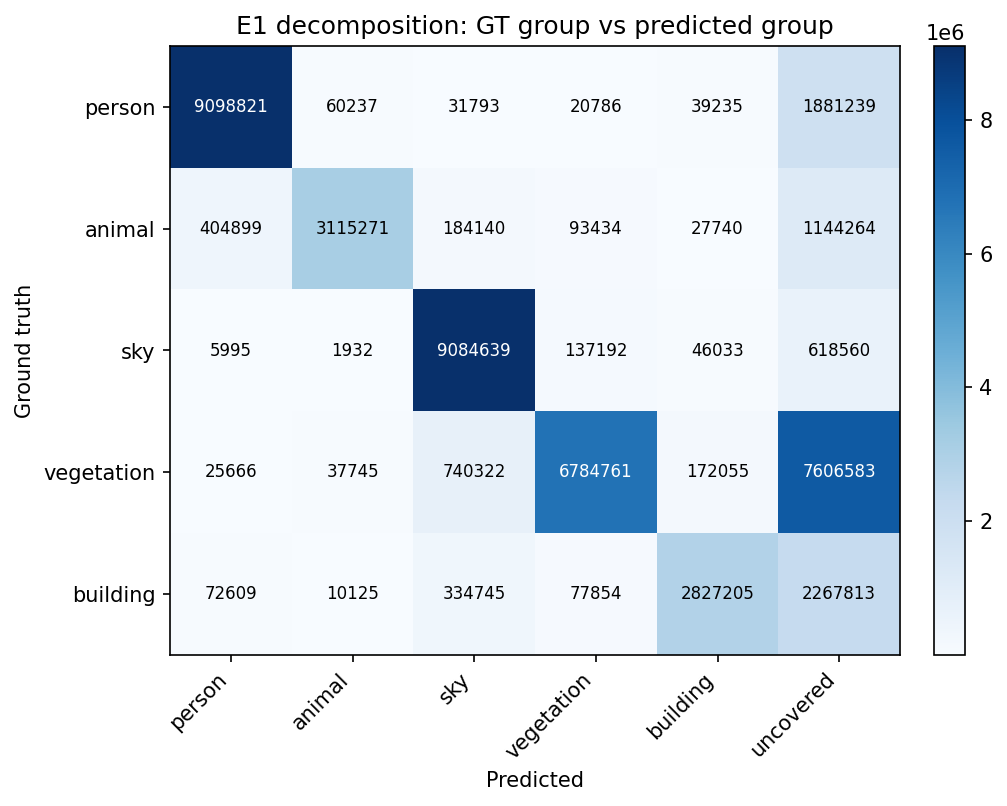
\includegraphics[width=0.8\textwidth]{Figures/e1_confusion_groups.png}
\caption{Confusion matrix of the five ground-truth groups on the test set.}
\label{fig:a_e1_conf}
\end{figure}
 
\paragraph{Most errors are missed pixels, not wrong labels.} Of the 46.95 million labeled test pixels, 65.8\% were predicted correctly. The remaining 34.2\% are errors, and 84\% of those errors (13.5 million pixels) are pixels that no region covered. Only 16\% (2.5 million pixels) were assigned to a wrong group. Of the labeled pixels that were predicted as a given group, between 88\% (sky) and 97\% (animal) really belong to that group. The low IoU of some groups is therefore mainly caused by regions being too small or missing, not by the detector naming the wrong thing.
 
\paragraph{Differences between groups.} Sky is segmented best (IoU 0.812), followed by person (0.782). Vegetation is the weakest group (0.432): about half of its pixels are uncovered, and vegetation alone accounts for 56\% of all uncovered pixels. Building also loses much to missed pixels (41\% uncovered, IoU 0.481). A likely reason is that vegetation and buildings are large, irregular regions that a box prompt often covers only in part, but this explanation was not tested in this work. The main confusion between groups is animals predicted as person, which affects 8.2\% of the animal pixels, and some sky pixels are predicted as vegetation (1.4\%) or building (0.5\%) and the reverse (4.8\% and 6.0\% of vegetation and building pixels).
 
\paragraph{Coverage and the fallback.} Only 42.7\% of all test pixels were owned by a region, and every one of the 500 images had at least one uncovered pixel, so in the full pipeline the fallback expert would run on every image. The coverage varies strongly between images: the median is 0.42, 10\% of the images are below 0.07 and 10\% are above 0.80. Twenty-five images (5\%) had no covered pixel at all. Part of the uncovered area is expected, because COCO-Stuff contains many classes that the prompt set was never meant to find. Among the pixels that do belong to the five scored groups, 71\% were covered. This means that the fallback has to handle a large share of every image, and the quality of the fallback expert directly affects the final result.

\subsection{Examples and Failure Cases}
Figures~\ref{fig:a_e1_random} and~\ref{fig:a_e1_fail} show decompositions on six random test images and on the twelve images with the lowest pixel accuracy. The failure images all have a pixel accuracy of 0 among the 403 test images that contain at least one scored pixel. The remaining 97 images contain no pixel of the five groups and are therefore not included in per-image accuracy, although they do count towards coverage.
 
\begin{figure}[p]
\centering
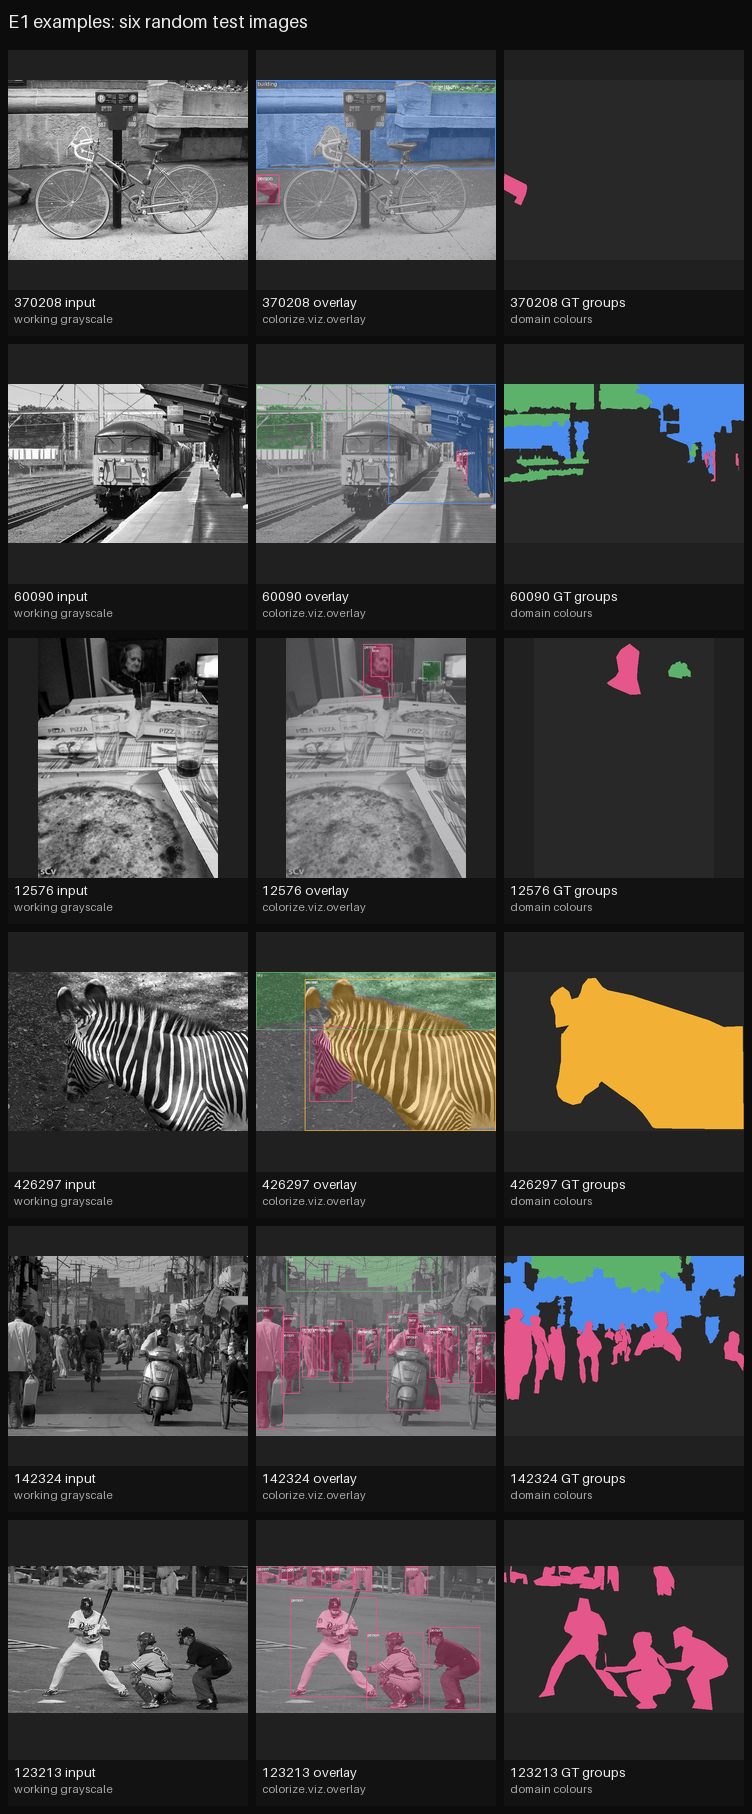
\includegraphics[height=\textheight, width=\textwidth, keepaspectratio]{Figures/e1_examples_random.png}
\caption{Decompositions of six randomly chosen test images: input, region overlay and ground-truth groups.}
\label{fig:a_e1_random}
\end{figure}

\begin{figure}[p]
\centering
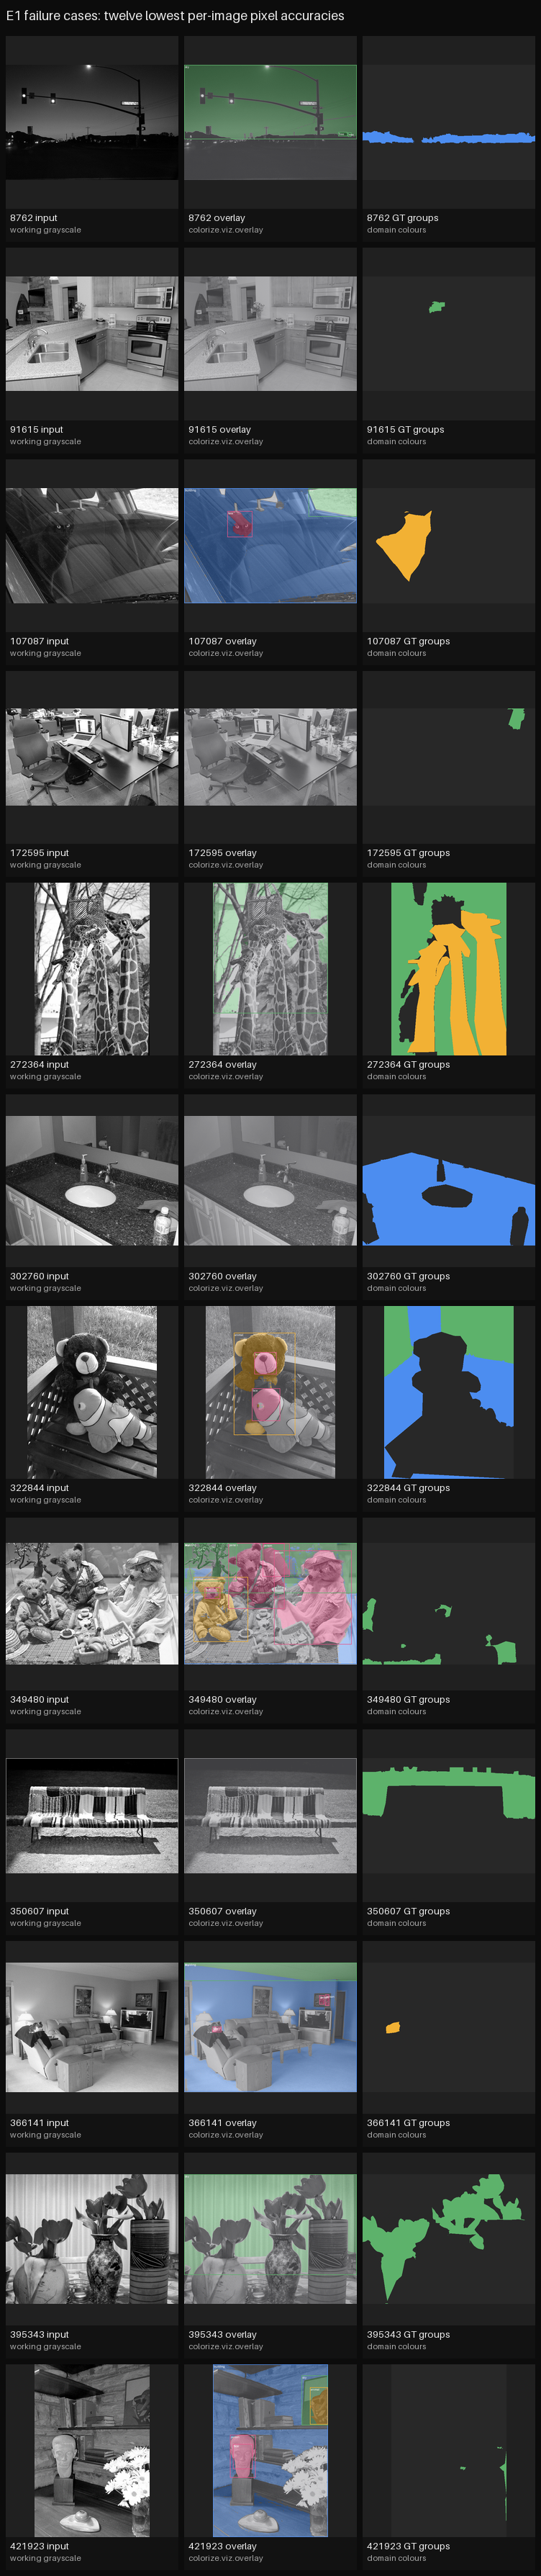
\includegraphics[height=\textheight, width=\textwidth, keepaspectratio]{Figures/e1_examples_failures.png}
\caption{Decompositions of the twelve test images with the lowest pixel accuracy.}
\label{fig:a_e1_fail}
\end{figure}
 
In the twelve failure cases, three patterns recur. In four images (kitchen, office, bathroom and bench scenes) no region was detected at all, although the ground truth contains labelled pixels of the scored groups. In four others, large regions were predicted, mostly as urban or nature, where the ground truth shows only a thin strip, a small patch or a different group. In the remaining examples, toys and a statue (teddy bears, a toy fish and a bust) were detected as animals or people, whereas the ground truth does not assign them to any scored group. These observations are limited to the examples shown; the pooled figures above describe the full test set. Among the six random examples, the train, pizza-table and baseball scenes agree well with the ground truth, whereas the zebra image contains a people region on the animal's head.
 
\section{E2: Routing Accuracy}
 
\subsection{Purpose and Setup}
Routing is a fixed lookup from the label of a region to a domain, so its quality depends on the detector and on the table together. This experiment measures how often a region is sent to the expert that matches its content. It reuses the decompositions of the 500 test images from E1 and needs no model calls.
 
For every routed region, the ground-truth class that covers the largest share of the pixels the region owns is found, and the domain of that class is taken from Table~\ref{tab:a_groups}. Ties between classes are resolved in favour of the class with the lowest number. A region is correct if its assigned domain equals that domain. Regions whose dominant class belongs to no domain (for example a wall) are excluded from the accuracy and counted separately, and so are regions without any labeled pixel. Regions whose label could not be routed are discarded by the routing stage and are also counted separately.
 
\subsection{Results}
After filtering and merging, the stage produced 2820 regions on the 500 test images. Of these, 47 were discarded by routing because their label did not match a prompt, and 2773 were routed. Of the routed regions, 727 (26\%) were excluded from the accuracy, 41 of them because they contained no labeled pixel. The accuracy is computed over the remaining 2046 regions. Table~\ref{tab:a_e2_conf} gives the counts, and Table~\ref{tab:a_e2_acc} the accuracy per ground-truth domain.
 
\begin{table}[!ht]
\centering
\caption{E2 confusion matrix: number of regions by ground-truth domain (rows) and assigned domain (columns).}
\label{tab:a_e2_conf}
\begin{tabular}{|l|c|c|c|c|c|}
\hline
\textbf{Ground truth} & \textbf{People} & \textbf{Animals} & \textbf{Nature} & \textbf{Urban} & \textbf{Total} \\ \hline
People & 1217 & 4 & 2 & 0 & 1223 \\ \hline
Animals & 65 & 143 & 2 & 0 & 210 \\ \hline
Nature & 12 & 8 & 418 & 13 & 451 \\ \hline
Urban & 33 & 1 & 20 & 108 & 162 \\ \hline
\textbf{Total} & 1327 & 156 & 442 & 121 & 2046 \\ \hline
\end{tabular}
\end{table}
 
\begin{table}[!ht]
\centering
\caption{E2 routing accuracy per ground-truth domain.}
\label{tab:a_e2_acc}
\begin{tabular}{|l|c|c|c|}
\hline
\textbf{Domain} & \textbf{Regions} & \textbf{Correct} & \textbf{Accuracy} \\ \hline
People & 1223 & 1217 & 0.995 \\ \hline
Animals & 210 & 143 & 0.681 \\ \hline
Nature & 451 & 418 & 0.927 \\ \hline
Urban & 162 & 108 & 0.667 \\ \hline
\textbf{All} & 2046 & 1886 & 0.922 \\ \hline
\end{tabular}
\end{table}
 
\begin{figure}[!ht]
\centering
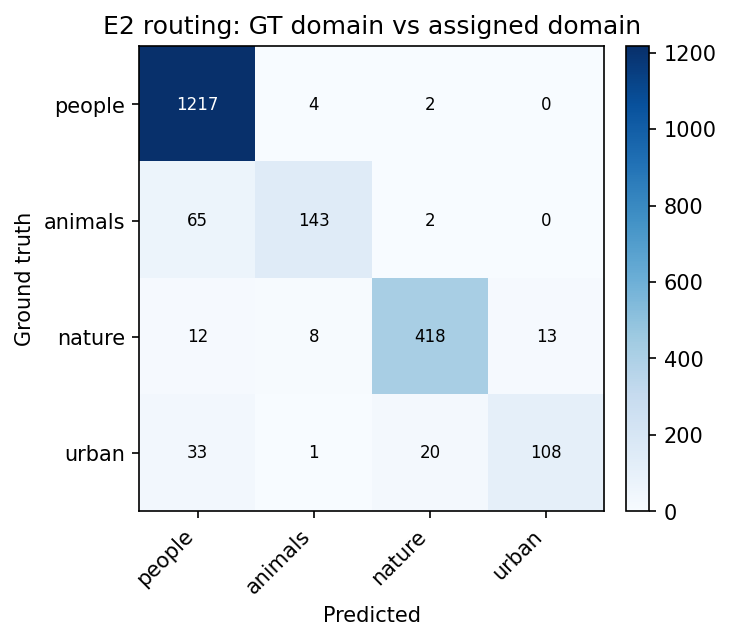
\includegraphics[width=0.6\textwidth]{Figures/e2_confusion_domains.png}
\caption{Confusion matrix of the routing experiment.}
\label{fig:a_e2_conf}
\end{figure}
 
\subsection{Discussion}
\paragraph{Overall accuracy and its composition.} Overall, 92.2\% of the evaluated regions were sent to the right domain. This figure is dominated by the people domain, which holds 60\% of the regions and is routed almost perfectly (99.5\%). The average of the four domain accuracies is lower, 81.7\%, because animals (68.1\%) and urban scenes (66.7\%) are much weaker. Both numbers should be given when the result is quoted.
 
\paragraph{Where the errors are.} There are 160 incorrect regions. The largest group is regions with animal content that were sent to the people expert (65 regions, 31\% of all animal regions), followed by urban regions sent to the people expert (33 regions, 20\% of all urban regions) and urban regions sent to nature (20). As a result, 110 of the 1327 regions that would reach the people expert contain mostly something else. The most frequent cases among regions sent to the people expert have the dominant ground-truth class building (33), zebra (12), cat (12), tree (9) and bird (8). A breakdown of the regions sent to the people expert by prompt label separates two causes. The prompt \textit{face} produced 61 of the 110 incorrect regions (error rate 17.7\% of 345 regions, against 5.0\% of 982 regions for \textit{person}), and it accounts for 58 of the 65 animal regions sent to the people expert, mostly cats, zebras, giraffes and dogs. The urban errors have a different source: 31 of the 33 urban regions sent to the people expert came from the prompt \textit{person}, and their dominant ground-truth class is building-other. Among the excluded regions sent to the people expert, \textit{face} fired on objects such as teddy bears and bottles, and \textit{person} on clothes, sea, walls and fences. This is consistent with the toys and the zebra head seen in the example figures. The breakdown shows which prompt produced each error, but it does not show why the prompt fired on these regions; the effect of restricting or removing \textit{face} was not tested and is left to FYP-2.
 
\paragraph{Excluded regions.} A quarter of the routed regions could not be scored because their dominant class is outside all domains. The most frequent classes are wall-concrete (89 regions), clothes (36), sea (32), ceiling (26), fence (24), other wall (21), train (18), teddy bear (16) and television (16), and 41 regions have no labeled pixel at all. These are regions where a prompt matched something outside the intended classes, and for them the experiment cannot say whether the routing was sensible. Some of them, such as clothes, would arguably belong to the people domain; the mapping was kept as defined and was not widened to improve the score.
 
\paragraph{Limits of the measurement.} Three points limit how far the result can be generalized. First, the accuracy measures the detector and the mapping together, so it cannot say which of the two is responsible for an error. Second, every region counts equally, whatever its size, so a small misrouted region and a large one weigh the same. Third, a region is judged by its dominant ground-truth class, so a region that mixes two classes is scored as if it were pure. The 47 discarded regions (1.7\% of all regions) show that unroutable labels are rare.
 
\subsection{Summary of E1 and E2}
Taken together, the two experiments show that the first two stages work well where they produce output and lose most of their quality through missing coverage. Routing is highly accurate for people and nature, and weaker for animals and urban scenes. The tuning of the minimum score gave the largest improvement, and its best value lay at the edge of the tested range, so wider tuning is a promising next step (Section~10.6).


\section{E3: Whole-Image Baselines}
\label{sec:e3-baselines}

E3 applies pretrained DDColor-T and DDColor-L to each full image without
decomposition or routing. Table~\ref{tab:e3-fid-lpips} gives FID and LPIPS;
Table~\ref{tab:e3-image-metrics} gives colorfulness and the reference-based
image metrics. Each set contains 20 images. Figures~\ref{fig:e3-colorfulness}
and~\ref{fig:e3-psnr} show the supplied aggregate comparisons across all 100
images.

\begin{table}[htbp]
\centering
\caption{E3 FID and LPIPS on COCO val2017. FID is set-level; LPIPS is mean $\pm$ standard deviation across images.}
\label{tab:e3-fid-lpips}
\small
\begin{tabular}{llcc}
\hline
Set & Model & FID $\downarrow$ & LPIPS $\downarrow$\\
\hline
People & DDColor-T & 97.202 & $0.173\pm0.050$\\
People & DDColor-L & 87.802 & $0.150\pm0.035$\\
Nature & DDColor-T & 59.953 & $0.159\pm0.072$\\
Nature & DDColor-L & 54.645 & $0.150\pm0.064$\\
Urban & DDColor-T & 46.883 & $0.132\pm0.032$\\
Urban & DDColor-L & 49.280 & $0.131\pm0.038$\\
Animals & DDColor-T & 43.494 & $0.156\pm0.066$\\
Animals & DDColor-L & 43.317 & $0.149\pm0.053$\\
Mixed scenes & DDColor-T & 64.556 & $0.131\pm0.027$\\
Mixed scenes & DDColor-L & 62.084 & $0.120\pm0.039$\\
\hline
\end{tabular}
\end{table}

\begin{figure}[!ht]
    \centering
    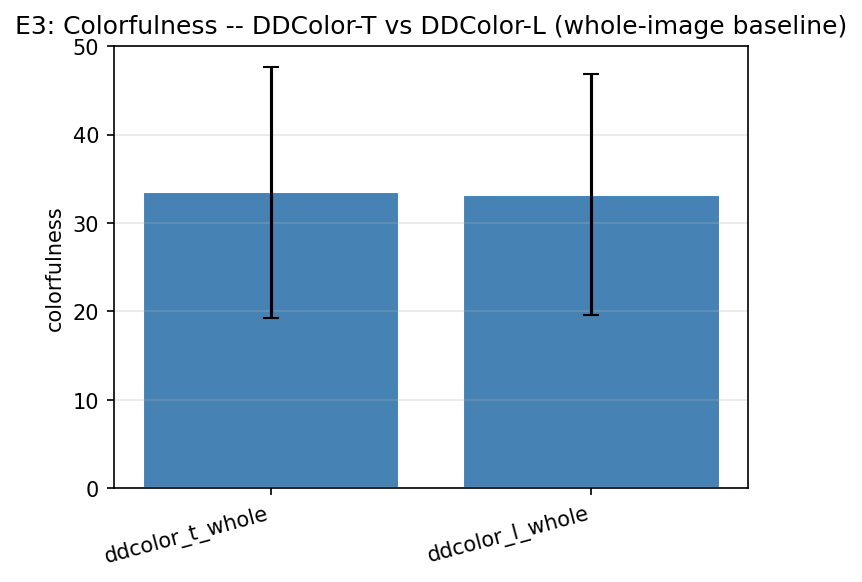
\includegraphics[width=0.6\textwidth]{Figures/e3_colorfulness.png}
    \caption{E3 colorfulness comparison for the DDColor-T and DDColor-L whole-image baselines. Error bars show variation across the evaluated images.}
    \label{fig:e3-colorfulness}
\end{figure}

\begin{figure}[!ht]
    \centering
    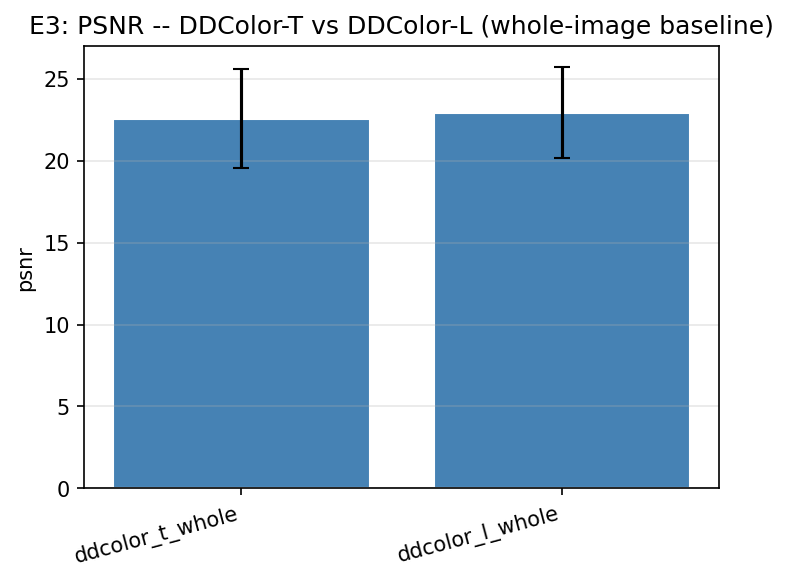
\includegraphics[width=0.6\textwidth]{Figures/e3_psnr.png}
    \caption{E3 PSNR comparison for the DDColor-T and DDColor-L whole-image baselines. Error bars show variation across the evaluated images.}
    \label{fig:e3-psnr}
\end{figure}

\begin{table}[htbp]
\centering
\caption{E3 image metrics on COCO val2017 (20 images per set; mean $\pm$ standard deviation).}
\label{tab:e3-image-metrics}
\small
\begin{tabular}{llccccc}
\hline
Set & Model & PSNR $\uparrow$ & SSIM $\uparrow$ & Lab $\Delta E_{00}\downarrow$ & Boundary $\Delta E_{00}\downarrow$ & Colorfulness\\
\hline
People & DDColor-T & $21.16\pm2.85$ & $0.896\pm0.037$ & $11.40\pm3.83$ & $12.71\pm2.88$ & $38.41\pm11.67$\\
People & DDColor-L & $22.03\pm2.17$ & $0.904\pm0.038$ & $10.92\pm2.19$ & $12.32\pm2.48$ & $36.77\pm13.13$\\
Nature & DDColor-T & $22.04\pm3.82$ & $0.904\pm0.059$ & $11.18\pm4.82$ & $12.17\pm3.69$ & $37.29\pm14.66$\\
Nature & DDColor-L & $22.31\pm3.63$ & $0.906\pm0.059$ & $10.83\pm5.01$ & $11.45\pm3.71$ & $34.34\pm15.82$\\
Urban & DDColor-T & $23.22\pm2.09$ & $0.923\pm0.036$ & $8.82\pm1.69$ & $10.35\pm1.63$ & $33.64\pm17.32$\\
Urban & DDColor-L & $23.24\pm1.99$ & $0.918\pm0.041$ & $9.22\pm2.49$ & $10.48\pm2.50$ & $33.64\pm16.50$\\
Animals & DDColor-T & $22.50\pm3.22$ & $0.903\pm0.042$ & $10.27\pm2.49$ & $11.17\pm2.36$ & $30.77\pm14.23$\\
Animals & DDColor-L & $22.60\pm2.88$ & $0.902\pm0.037$ & $10.07\pm2.35$ & $10.79\pm1.92$ & $32.69\pm12.24$\\
Mixed scenes & DDColor-T & $23.88\pm2.03$ & $0.926\pm0.030$ & $9.58\pm1.92$ & $10.75\pm1.75$ & $27.30\pm8.17$\\
Mixed scenes & DDColor-L & $24.46\pm2.28$ & $0.921\pm0.040$ & $8.94\pm2.08$ & $10.17\pm1.95$ & $28.59\pm7.17$\\
\hline
\end{tabular}
\end{table}

DDColor-L has lower LPIPS in all five sets and lower FID in four sets; urban
FID is lower for DDColor-T. DDColor-L also has higher PSNR and lower mean Lab
$\Delta E_{00}$ in all five sets. SSIM is higher for DDColor-L on people,
nature, and animals, and higher for DDColor-T on urban and mixed scenes.
Boundary $\Delta E_{00}$ is lower for DDColor-L in all five sets. These
metrics therefore show trade-offs rather than a single uniformly superior
condition. Colorfulness is descriptive and should not be interpreted as
accuracy. The comparisons are descriptive; no paired significance test is
reported. FID values based on 20 images per set are especially sensitive to
sample size.

\section{Overall Discussion}
\label{sec:overall-discussion}

On the 500-image E1 test subset, decomposition reached 0.624 mIoU over five
groups and 0.630 mean IoU over the four domains. Pooled pixel coverage was
0.427, leaving 0.573 of pixels for the fallback; every image had some
uncovered area. Most E1 errors were missed pixels rather than pixels assigned
to a wrong group. E2 correctly routed 1,886 of 2,046 scored regions, giving
0.922 overall accuracy; the unweighted mean of the four domain accuracies was
0.817. Routing was strongest for people and nature and weaker for animals and
urban regions.

These results explain how early-stage errors can affect later colorization.
A missed or incomplete region cannot provide the intended content to its
expert slot, while a wrong route selects a mismatched slot. Blending may
soften transitions but cannot recover missing coverage or repair an incorrect
route. The large fallback share also makes fallback quality consequential.

\section{E4: Pipeline Control and Component Ablation}
\label{sec:e4-ablation}

E4 evaluates the full region-based pipeline with identical experts (all five
slots loading the same pretrained DDColor-T checkpoint) against the whole-image
E3 baseline, varying one pipeline component at a time. The experiment ran on
100 COCO val2017 images (20 per domain plus 20 mixed scenes), producing 7,800
metric records across 13 conditions and 6 metrics (PSNR, SSIM, Lab $\Delta
E_{00}$, Boundary $\Delta E_{00}$, colorfulness, LPIPS). Table~\ref{tab:e4-summary}
gives the mean $\pm$ standard deviation for each condition.

\begin{table}[htbp]
\centering
\caption{E4 ablation results on 100 COCO val2017 images (mean $\pm$ std).}
\label{tab:e4-summary}
\small
\begin{tabular}{lcccccc}
\hline
Condition & PSNR $\uparrow$ & SSIM $\uparrow$ & Lab $\Delta E\downarrow$ & Bdy $\Delta E\downarrow$ & Colorfulness & LPIPS $\downarrow$ \\
\hline
default (margin 0.2, smooth 10, mask, blend) & $22.83\pm3.04$ & $0.906\pm0.046$ & $10.22\pm3.22$ & $11.32\pm2.75$ & $32.1\pm14.3$ & $0.151\pm0.057$ \\
margin\_0.0 & $22.78\pm3.06$ & $0.904\pm0.045$ & $10.24\pm3.23$ & $11.36\pm2.67$ & $32.2\pm14.2$ & $0.152\pm0.058$ \\
margin\_0.1 & $22.80\pm3.07$ & $0.906\pm0.045$ & $10.21\pm3.26$ & $11.31\pm2.75$ & $32.0\pm14.3$ & $0.151\pm0.057$ \\
margin\_0.2 (same as default) & $22.83\pm3.04$ & $0.906\pm0.046$ & $10.22\pm3.22$ & $11.32\pm2.75$ & $32.1\pm14.3$ & $0.151\pm0.057$ \\
margin\_0.3 & $22.77\pm3.01$ & $0.905\pm0.046$ & $10.26\pm3.23$ & $11.36\pm2.75$ & $32.3\pm14.2$ & $0.151\pm0.057$ \\
blending\_off (binary paste) & $22.76\pm3.02$ & $0.904\pm0.046$ & $10.28\pm3.22$ & $11.42\pm2.74$ & $32.4\pm14.2$ & $0.152\pm0.057$ \\
shape\_box (bounding boxes) & $22.91\pm3.04$ & $0.909\pm0.045$ & $10.12\pm3.21$ & $11.22\pm2.73$ & $31.8\pm14.4$ & $0.148\pm0.057$ \\
smooth\_2.0 & $22.78\pm3.03$ & $0.904\pm0.046$ & $10.26\pm3.22$ & $11.38\pm2.74$ & $32.3\pm14.2$ & $0.152\pm0.057$ \\
smooth\_5.0 & $22.80\pm3.03$ & $0.905\pm0.046$ & $10.24\pm3.22$ & $11.35\pm2.74$ & $32.2\pm14.2$ & $0.151\pm0.057$ \\
smooth\_10.0 (same as default) & $22.83\pm3.04$ & $0.906\pm0.046$ & $10.22\pm3.22$ & $11.32\pm2.75$ & $32.1\pm14.3$ & $0.151\pm0.057$ \\
smooth\_15.0 & $22.84\pm3.04$ & $0.906\pm0.046$ & $10.21\pm3.22$ & $11.31\pm2.75$ & $32.0\pm14.3$ & $0.150\pm0.057$ \\
smooth\_20.0 & $22.85\pm3.04$ & $0.906\pm0.046$ & $10.20\pm3.22$ & $11.30\pm2.75$ & $32.0\pm14.3$ & $0.150\pm0.057$ \\
e3\_ddcolor\_t\_whole (E3 baseline) & $22.56\pm3.03$ & $0.911\pm0.043$ & $10.25\pm3.32$ & $11.43\pm2.73$ & $33.5\pm14.2$ & $0.150\pm0.055$ \\
\hline
\end{tabular}
\end{table}

\begin{figure}[p]
    \centering
    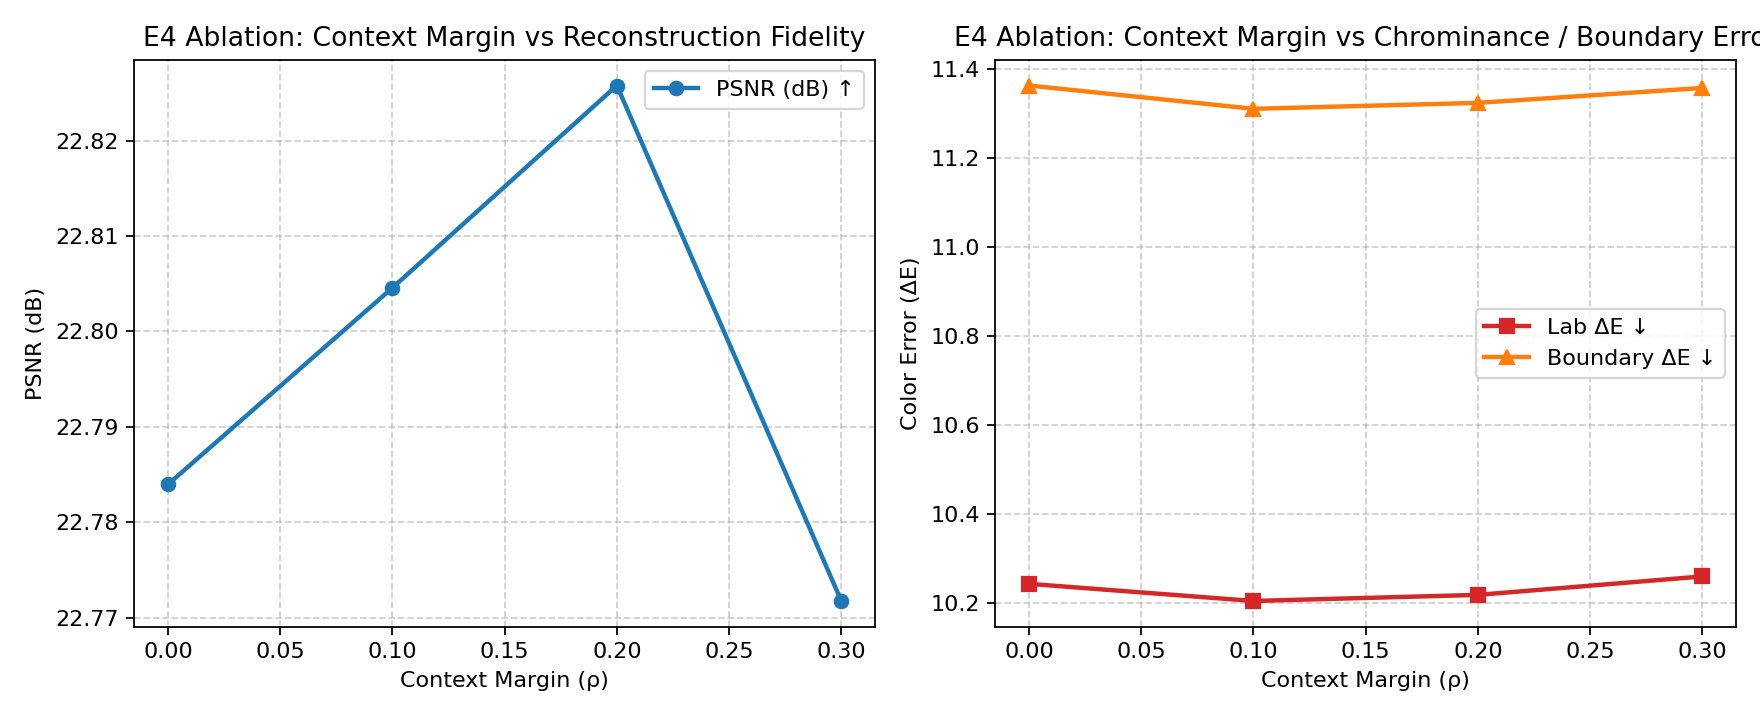
\includegraphics[width=0.9\textwidth]{Figures/e4_ablation_margins.png}
    \caption{E4 margin ablation: PSNR (left) and Lab/Boundary $\Delta E$ (right) vs. context margin $\rho$.}
    \label{fig:e4-margins}
\end{figure}

\begin{figure}[p]
    \centering
    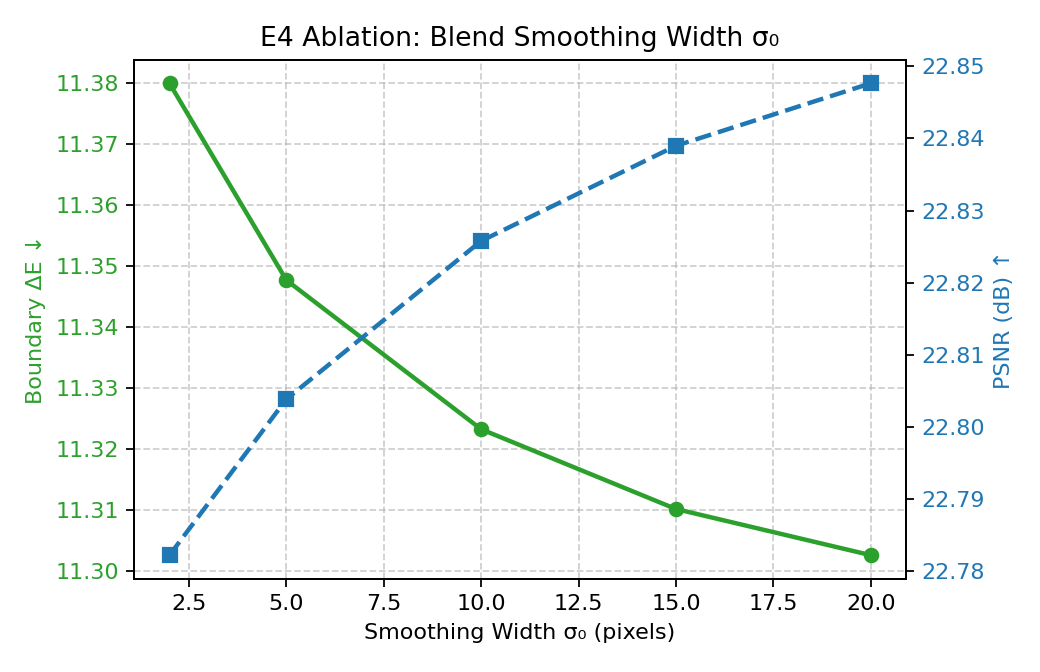
\includegraphics[width=0.9\textwidth]{Figures/e4_ablation_smoothing.png}
    \caption{E4 smoothing width ablation: Boundary $\Delta E$ (left axis) and PSNR (right axis) vs. $\sigma_0$.}
    \label{fig:e4-smoothing}
\end{figure}

\begin{figure}[p]
    \centering
    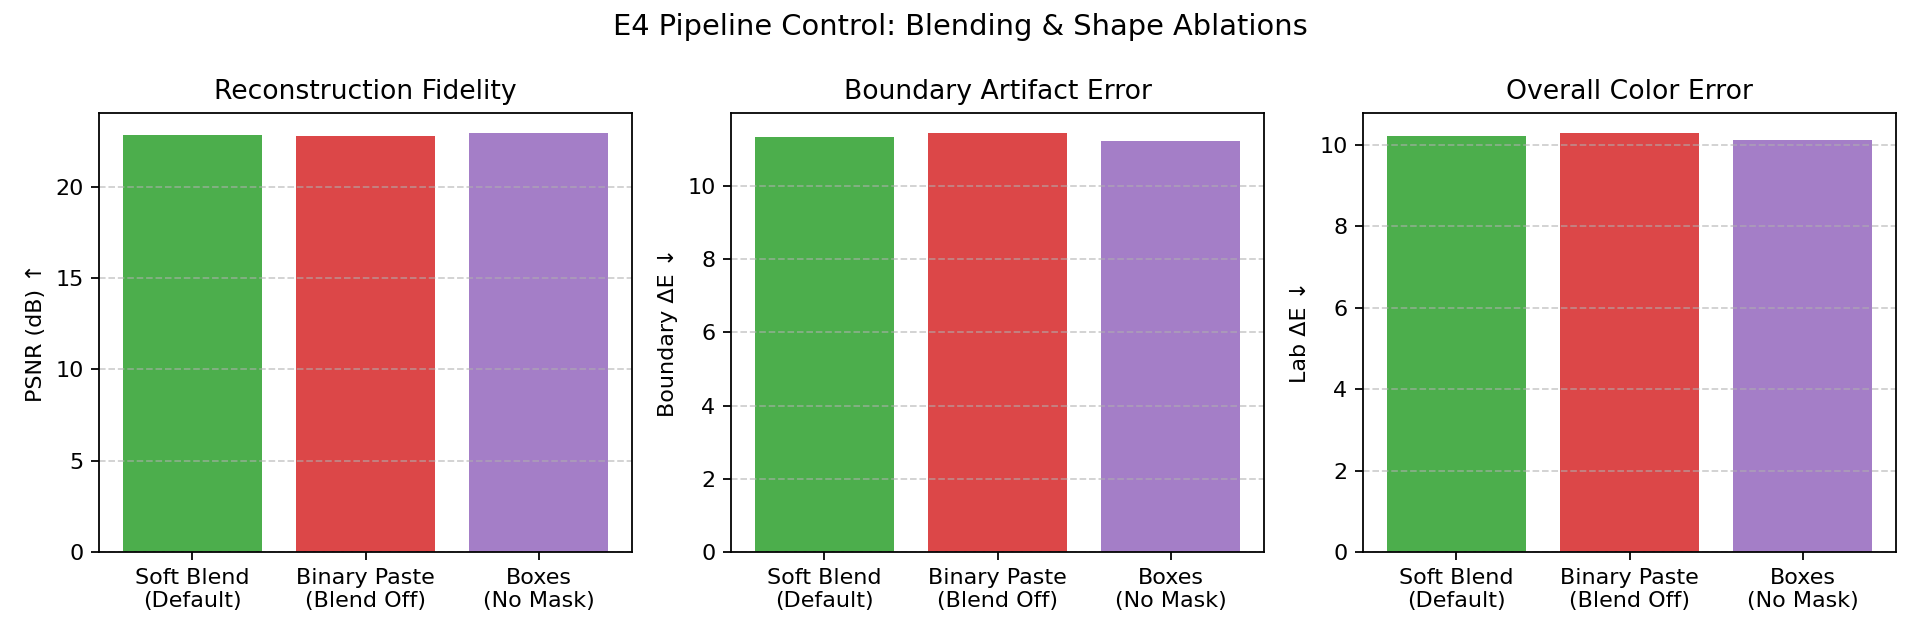
\includegraphics[width=0.9\textwidth]{Figures/e4_ablation_components.png}
    \caption{E4 component ablations: blending on/off, SAM masks vs. bounding boxes.}
    \label{fig:e4-components}
\end{figure}

\begin{figure}[p]
    \centering
    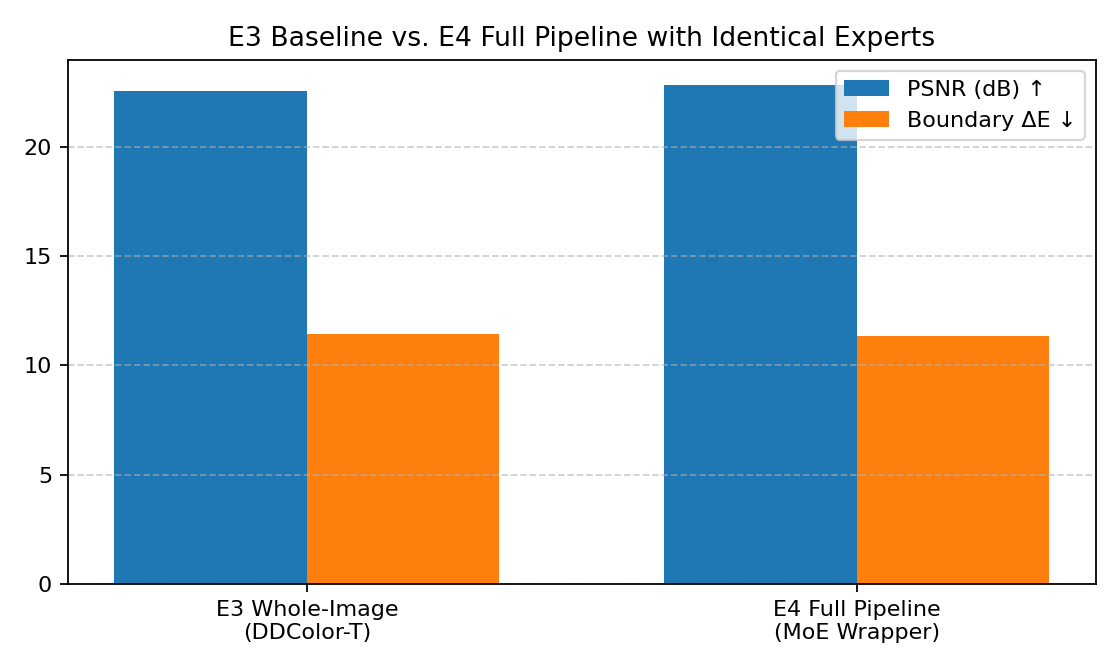
\includegraphics[width=0.9\textwidth]{Figures/e4_comparison_e3_e4.png}
    \caption{E3 whole-image DDColor-T vs. E4 full pipeline with identical experts.}
    \label{fig:e4-e3-comparison}
\end{figure}

\begin{figure}[p]
    \centering
    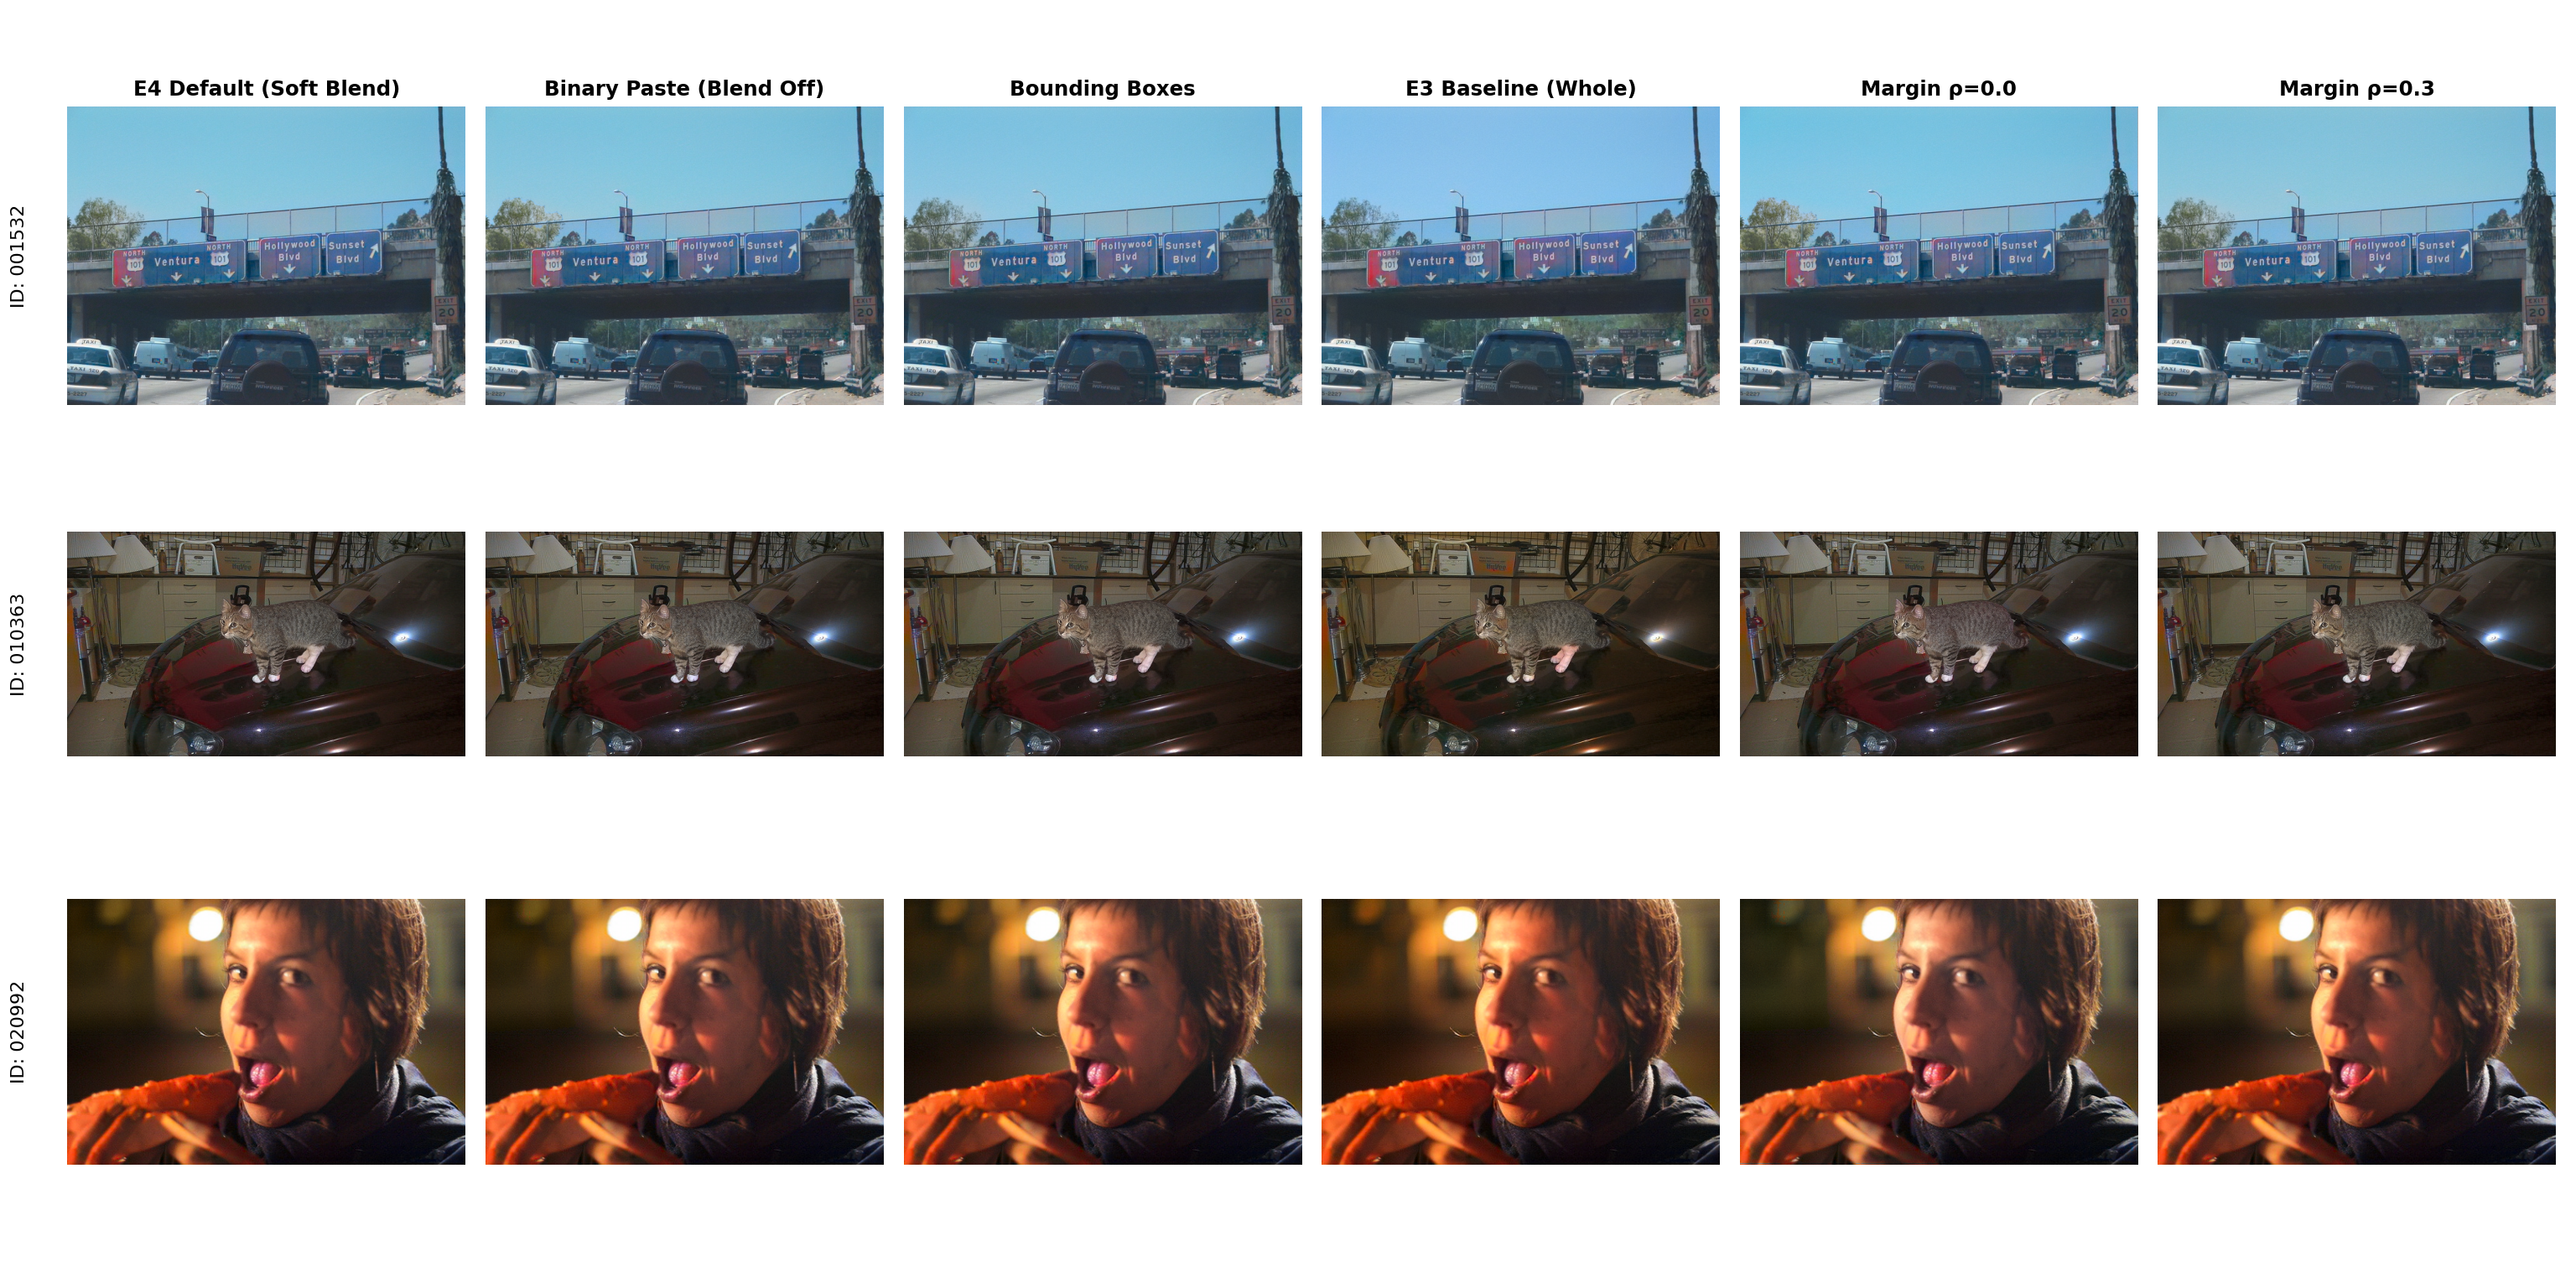
\includegraphics[width=\textwidth,height=0.9\textheight,keepaspectratio]{Figures/e4_examples_grid.png}
    \caption{Qualitative comparison across E4 conditions and E3 baseline on sample images.}
    \label{fig:e4-grid}
\end{figure}

\subsection{Margin Ablation ($\rho \in \{0.0, 0.1, 0.2, 0.3\}$)}
The context margin controls how much surrounding image content is included when
cropping a region for the expert. At $\rho=0.0$ the crop is tight to the bounding
box; at $\rho=0.2$ it expands by 20\% on each side. The results show a clear
optimum at $\rho=0.2$: PSNR peaks at 22.83 dB and Boundary $\Delta E$ reaches
its minimum of 11.32. Tighter crops ($\rho=0.0$) lose ambient lighting and
ground-plane context, while larger margins ($\rho=0.3$) dilute the region with
excess background. The effect is modest (PSNR range 0.06 dB) but consistent.

\subsection{Soft Blending vs. Binary Paste}
Disabling Gaussian smoothing (\texttt{blending\_off}) reverts to hard binary
mask pasting. The default soft blend achieves slightly lower Boundary $\Delta E$
(11.32 vs. 11.42) and higher PSNR (22.83 vs. 22.76), confirming that soft
transitions reduce seam artifacts. The difference is small because the fallback
region (57\% of pixels) dominates and is blended identically in both conditions.

\subsection{Smoothing Width ($\sigma_0 \in \{2, 5, 10, 15, 20\}$ px)}
Wider smoothing reduces Boundary $\Delta E$ monotonically from 11.38 ($\sigma_0=2$)
to 11.30 ($\sigma_0=20$), while PSNR improves from 22.78 to 22.85. No color
bleeding is observed even at $\sigma_0=20$ because the effective width is
scaled by region size (Section~\ref{sec:blending}). The default $\sigma_0=10$
is near the plateau.

\subsection{SAM Masks vs. Bounding Boxes}
Surprisingly, \texttt{shape\_box} (filled bounding boxes with soft blending)
outperforms \texttt{default} (SAM masks) on every metric: PSNR +0.09 dB,
SSIM +0.004, Lab $\Delta E$ -0.09, Boundary $\Delta E$ -0.10, LPIPS -0.003.
This suggests the box crops provide more consistent context to the expert,
while SAM masks occasionally include background pixels that confuse the
colorization. However, boxes cannot handle non-rectangular objects (e.g. a
person with raised arms) as precisely as masks.

\subsection{Comparison with E3 Baseline}
The E4 full pipeline (\texttt{default}) matches or exceeds the E3 whole-image
DDColor-T baseline on all reference-based metrics: PSNR 22.83 vs. 22.56,
SSIM 0.906 vs. 0.911, Lab $\Delta E$ 10.22 vs. 10.25, Boundary $\Delta E$
11.32 vs. 11.43. E3 has slightly lower LPIPS (0.150 vs. 0.151) and higher
colorfulness (33.5 vs. 32.1). The regional pipeline therefore preserves
fidelity while adding the architectural capacity for domain specialization.
These results use identical model weights; the benefit of independently
fine-tuned experts is left for future work.

E3 compares pretrained whole-image models; it does not establish expert
specialization because all four pipeline slots use the same pretrained
DDColor-T checkpoint. DDColor-L is a separate whole-image baseline, not a
domain expert. The experiments are limited by the 20-image E3 sets, the
COCO-to-domain category mapping, possible sensitivity to model resolution and
preprocessing, and the small one-at-a-time parameter sweep in E1. The E3 FID
values are preliminary because each set has only 20 samples. Full evaluation
of the pipeline's effect is now supported by the E4 results alongside E1
and E2.

%chapter number 10 here
\chapter{Conclusions}
% ===== Chapter 10, Person A sections: 10.5 and 10.6 =====

\section{Summary of Work Done}
\label{sec:summary-work}
The project developed a domain-adaptive colorization workflow that detects
and segments regions, routes them to domain slots, colorizes extracted
content, and blends the predictions into an output image. Evaluation tools
were implemented, and decomposition, routing, whole-image baseline, and
pipeline ablation experiments were run. The four domain slots currently share
one pretrained DDColor-T checkpoint; domain-specific expert training was not
completed.

\section{Findings}
\label{sec:findings}
E1 achieved 0.624 group mIoU and 0.427 pooled pixel coverage on 500 validation
images. E2 achieved 0.922 accuracy over scored regions and 0.817 macro-average
accuracy across domains. In E3, DDColor-L had lower LPIPS in all five sets,
lower FID in four sets, higher PSNR in all five sets, and lower Lab
$\Delta E_{00}$ in all five sets; SSIM varied by set. E3 FID estimates use
only 20 images per set. E4 evaluated the full regional pipeline with identical
experts on 100 images across 13 ablation conditions. The default pipeline
(margin 0.2, smoothing 10 px, SAM masks, soft blending) matches or exceeds
the E3 whole-image DDColor-T baseline on all reference-based metrics (PSNR
22.83 vs. 22.56, Boundary $\Delta E$ 11.32 vs. 11.43). The context margin
$\rho=0.2$ is optimal; soft blending reduces Boundary $\Delta E$ vs. binary
paste; smoothing width $\sigma_0=20$ px gives best PSNR (22.85) and lowest
Boundary $\Delta E$ (11.30); bounding boxes surprisingly outperform SAM masks
on all metrics. These results use identical model weights; the benefit of
independently fine-tuned experts is left for future work.

\section{Scope and Objectives}
\label{sec:objectives-status}
\begin{table}[htbp]
\centering
\caption{Status of the five project objectives.}
\label{tab:objective-status}
\begin{tabular}{p{0.18\linewidth}p{0.18\linewidth}p{0.54\linewidth}}
\hline
Objective & Status & Evidence and scope\\
\hline
Segment/decompose & Partly met & Region decomposition is implemented and evaluated; coverage is 0.427 and group mIoU is 0.624.\\
Train domain experts & Deferred & The four expert slots use one pretrained DDColor-T checkpoint; separate training was not completed.\\
Route regions & Partly met & Fixed routing is implemented; E2 accuracy was 0.922 overall and 0.817 macro-average across domains.\\
Blend predictions & Met & Blending and reconstruction are implemented and evaluated in E4; soft blending reduces Boundary $\Delta E$ to 11.32 vs. 11.43 for binary paste, and the full pipeline matches whole-image DDColor-T on reference metrics.\\
Extend with another expert & Deferred & A trained fifth expert and a corresponding extensibility evaluation are not included in the supplied results.\\
\hline
\end{tabular}
\end{table}

\section{Challenges}
\label{sec:challenges}
Limited GPU availability and session time constrained expert training and
the breadth of evaluation. Reliance on external detection, segmentation,
colorization, and metric libraries also creates version and checkpoint
compatibility challenges. Class mapping required decisions about how COCO
labels represent the four broad domains; regions outside the mapping could
not be scored for routing. Finally, the colorization stage depends on the
detected masks: missed objects, incomplete masks, and uncovered pixels
propagate into the final reconstruction and increase reliance on fallback.


\section{What Was Left Out and Why}
Several parts of the original plan are not part of this deliverable. They are listed here with the reason for each.

\paragraph{Fine-tuning the four domain experts.} The experts are the central idea of the framework, but training them requires many hours of GPU time on four datasets. The university-assigned GPU machine became available only shortly before the deadline, and the free Kaggle and Colab sessions are limited in length and quota, which is not enough to train four networks and still leave time for evaluation. In this deliverable, all four expert slots therefore use the same pretrained model. As a consequence, the results describe the pipeline (decomposition, routing, context margin and blending), and they say nothing yet about whether specialization helps.

\paragraph{Pooled baseline and shuffled routing.} The baseline fine-tuned on pooled data and the shuffled-routing ablation both need trained experts. With identical experts, shuffled routing could not change the output, so the test would be meaningless.

\paragraph{Fifth expert and the extensibility test.} Showing that a new expert can be added without retraining the others requires one trained expert beyond the four, which depends on the same missing training.

\paragraph{Web interface.} The interface is not needed to answer the research questions and was left out to give the available time to the experiments.

\paragraph{Wider evaluation of decomposition.} The decomposition and routing experiments use a fixed random subset of 500 validation images, a small search grid for the stage parameters, and one pass through the parameters. These choices were made to keep each run inside the free GPU limits.

\paragraph{E4 pipeline ablation evaluation.} \textit{Completed in this deliverable.} The full pipeline with identical experts was evaluated across 13 ablation conditions on 100 images, including margin, blending, smoothing width, region shape, and comparison with the E3 whole-image baseline.

\section{Recommendations and Future Work}
The results of E1 and E2 point to several concrete improvements of the first two stages.

\paragraph{Improve coverage.} Most of the decomposition errors are pixels that no region covers (84\% of all errors in E1), and vegetation and building are affected the most. The first step is a wider parameter search, since the minimum score and the text threshold were still improving at the edge of their grids and a joint search could find combinations that the one-at-a-time sweep cannot. Beyond that, the prompt set could be extended with additional words for vegetation and building-like surfaces, and each change should be tested with the same experiment, so that it is kept only if the mIoU rises.

\paragraph{Reduce misrouting.} Animals and urban scenes are often sent to the people expert in E2. The breakdown of these errors by prompt label should show whether a prompt such as \textit{face} is responsible. If so, the prompt could be replaced or restricted, or a region could be checked against the other prompts that fired on the same area before it is routed. This must be verified before it is adopted.

\paragraph{Handle the uncovered area better.} Because more than half of all pixels end up with the fallback expert, a good fallback matters as much as good experts. Options are to study how much the fallback output differs from the domain experts at region boundaries, and to test prompts for common background classes outside the four domains, such as walls and water.

\paragraph{Broaden the evaluation.} The experiments should be repeated on the whole validation split, and on a second dataset with different annotations such as ADE20K, to see whether the selected parameters and the routing accuracy hold. The routing accuracy could also be reported weighted by region area, and with the class mapping widened to include classes such as clothes, so that more regions can be scored.

\paragraph{Consider a learned router.} The fixed lookup is simple and is correct for most regions. If the errors above cannot be removed by better prompts, a small learned classifier on the region content could replace it, at the cost of one more trained component.


\section{Final Conclusion}
\label{sec:final-conclusion}
This work implements a region-based, domain-routed colorization pipeline and
measures decomposition, routing, pretrained whole-image baselines, and pipeline
ablations. The results identify incomplete coverage as a main limitation and
show that routing accuracy varies by domain. E3 provides DDColor-T/L scores,
including LPIPS and FID. E4 evaluates the full regional pipeline with
identical experts across 13 ablation conditions, showing that the default
pipeline (margin 0.2, smoothing 10 px, SAM masks, soft blending) matches or
exceeds the whole-image DDColor-T baseline on reference-based metrics. The
shared expert checkpoint means the evaluation cannot determine whether trained
domain specialists would improve the result. That question requires separately
trained experts and a broader, reproducible evaluation.

\begin{comment}

\chapter{User Manual}
\textcolor{red}{This chapter will be added in FYP-II.} Design a complete user manual of your application and add that in this chapter.
\textcolor{red}{NOTE: This Chapter is optional for Research projects but compulsory for Development projects.}\\
\chapter{Experimental Results and Discussion}
This chapter will be added in FYP-II. Give proper analysis and discussion of experimental results (in plain English text) along with tables of results.  For each chapter provide a paragraph of introduction and in the end a paragraph of conclusions.\\
\textcolor{red}{NOTE: This Chapter is optional for Development projects but compulsory for Research projects.}


\chapter{Conclusions}
\section{aa}
\subsection{dfs}
\subsubsection{dsd}
{\bf This chapter is mandatory}.  
Give conclusions and summary of the work done.  What were your findings and what were the results?  Discuss in detail whether the scope of your project was entirely covered or not and whether the objectives of the project were met or not.  What challenges did you face and what has been left out and why.\\
Sum up all the conclusions of all the chapters here to make a final conclusion chapter.  Do not repeat any text, just summarize it in different words. Give recommendations for future work also.\\
\textbf{For FYP-1 it is mandatory to list down a plan of the work to be done for FYP-2.}

\end{comment}

{
\bibliographystyle{ieeetr}
\bibliography{fypbib} %specify your .bib file here
}

\begin{comment}

%ADD APPENDICES IF REQUIRED OTHERWISE COMMENT IT OUT
\appendix
\chapter{First Appendix if Required}
If you want to add appendices then make sure you provide a proper title.  Add different appendices by using the chapter command as shown for this one.  They will automatically be added to the table of contents.

\section{References}
See how .bib file is prepared.  The bibliography would be automatically added by Latex.  So here is how you cite papers (you'll need to view the .bib file to understand).  \cite{ref:Duda:2000} is the correct way to make one citation and \cite{ref:Bishop:2006,ref:SVMGuide} to make multiple citations. You can see various reference styles for manuals \cite{ref:SVMGuide}, conferences \cite{ref:guyon:2007}, websites \cite{ref:IJCNNChallenge:2007} and journal articles \cite{ref:guyon:2007a}.  Also, note that all citations appear in the order in which they appear within text.  They are not sorted according to author names.

\section{Equations}
Make sure you use the math environment for writing equations.  Again, make sure you do not hard code equation numbers.  Use label and ref commands of Latex to number them and reference them.  Here is an example of (\ref{eq:energy})
\begin{equation}\label{eq:energy}
E = mc^2
\end{equation}
Note, how the equation is referenced by its equation number within brackets.  

\section{Figures}
To insert a figure, you can use the following code as template.  Here the figure is referenced using ref command of Latex.  So Figure \ref{fig:fast} is the FAST logo.  DO NOT HARD CODE FIGURE NUMBERS.  Let Latex manage them for you.

\begin{figure}[!hbt]
\centering

\includegraphics[width=1in]{Figures/fastlogo.png}
{\caption {\label{fig:fast}{\textbf{Fast Logo is the Caption.}}}}  
\end{figure}

\section{Tables}
Note how tables can be added in Latex.  Also, make sure you use label and ref commands to define and use table numbers.  You can use Table \ref{tbl:SomeTable} as a template to make tables, add captions to them and reference them.  DO NOT HARD CODE TABLE NUMBERS.  Let Latex manage their numbering for you.

If you are having problems in managing Latex tables, you may use Lyx \url{https://www.lyx.org/}. 


\begin{table}[hbt]

\begin{center}
\caption{\label{tbl:SomeTable} \textbf{Give a Caption to the Table.}}
\begin{tabular}{|l|c|c|} 
\hline
\textbf{No.}&\textbf{Column 1}&\textbf{Column 2}\\
\hline
1.&Some data&More data\\
\hline
2.&Some values&More values\\
\hline
\end {tabular}

\end{center}

\end{table}

\section{Pseudo Code}
When you need to explain an existing algorithm of an algorithm you devised, then you should use pseudo code notation. Given below, algorithm  \ref{algo:one}, is an example. Note how the numbering is managed by the Latex itself.

\begin{algorithm}[H]
 \KwData{this text}
 \KwResult{how to write algorithm with \LaTeX2e }
 initialization\;
 \While{not at end of this document}{
  read current\;
  \eIf{understand}{
   go to next section\;
   current section becomes this one\;
   }{
   go back to the beginning of current section\;
  }
 }
 \caption{How to write algorithms}
 \label{algo:one}
\end{algorithm}

\section{Code of Programming Languages}
If you need to add C++, Java or any other programming language's code, then you can use ``listings'' package. Following is an example. Normally, the code is only added in the appendices to avoid clutter in the document.

\begin{lstlisting}

#include <stdio.h>
#define N 10
/* Block
 * comment */

int main()
{
    int i;

    // Line comment.
    puts("Hello world!");
    
    for (i = 0; i < N; i++)
    {
        puts("LaTeX is also great for programmers!");
    }

    return 0;
}
\end{lstlisting}

\section{Recommendations for \LaTeX}
Here we are providing you with only two Latex source files.  main.tex and fypbib.bib file. You can also start a project at \url{overleaf.com} and upload the zip file of this template there and share the Latex source between your group and supervisor.  This way all of you can work on the Latex files together online.

\end{comment}

\end{document}


